% Chapter 10

\chapter{Background Estimation} % Chapter title
\label{ch:backgrounds} 

This analysis requires two leptons with \mll~consistent with the $Z$ mass, at least two jets, large \met, and large \HT. Any \ac{SM} processes that produce this signature will appear as a background to the search. The most important task of the analysis is to identify and estimate these backgrounds, so that any excess of events appearing on top of the standard model background can be identified. The main backgrounds processes for this analysis are described in \autoref{ch:background_processes}. The largest background is from flavor symmetric processes, with smaller contributions coming from the remaining diboson processes, \dyjets, rare top processes, and fake and non-prompt leptons.

%----------------------------------------------------------------------------------------

\section{Flavor Symmetric Processes}
\label{sec:bg-fs}

The \ac{FS} background estimation is performed using two methods. The first, the Flavor Symmetry method, takes advantage of the uncorrelated lepton flavors in these processes, and uses data observed in the $e\mu$ channel to predict backgrounds in the $ee$ and $\mu\mu$ channels. The second, the Sideband Fit method, normalizes \ac{MC} using data in the off-$Z$ region of the $ee$ and $\mu\mu$ channels, and uses that normalization to make a prediction of the on-$Z$ region. Because it depends less on \ac{MC}, and because it has smaller total uncertainties (as discussed in \autoref{ch:background_uncertainties}), the Flavor Symmetry method is chosen as the nominal prediction, with the Sideband Fit method used as a cross-check.

%\acf{FS} backgrounds include any processes that produce pairs of leptons with uncorrelated flavor in the final state. In this analysis, the largest contribution comes from \ttbar, with additional events from processes like $WW$ and $Z\rightarrow\tau\tau$. In these processes, each lepton comes from a decay of different particles. In the case of \ttbar, the two top quarks decay to $W$ bosons, which each produce a lepton in their decays, as shown in \autoref{fig:ttbar}. These leptons' flavors are correlated with the flavor of the neutrino that results from the same boson's decay, but not with one another. %Unlike a $Z\rightarrow \ell\ell$ decay, these leptons' flavors are completely independent. 

\subsection{Flavor Symmetry Method}
\label{sec:method-fs}
As a consequence of the independence of the lepton flavors, any \ac{FS} process should produce $ee$, $\mu\mu$, and $e\mu$ events in a 1:1:2 ratio. This ratio is taken advantage of in the flavor symmetry method by measuring $e\mu$ events in data and using them to predict the contribution of these processes in the $ee$ and $\mu\mu$ channels \cite{SUSY-2014-10}.

To estimate the number of events in SRZ, a control region called CR-FS is used. Both regions are defined in \autoref{tab:regions-z}. CR-FS is very similar to SRZ with two changes: it requires different-flavor leptons instead of the same-flavor leptons required by SRZ, and the \mll~range it covers has been expanded by a factor of three, now ranging from 61 to 121 \gev. The expansion of the \mll~window is done to increase the number of events in the control region, thus lowering the statistical uncertainty of the prediction
\footnote{This method was developed for a smaller dataset for which this statistical uncertainty was the dominant uncertainty on the total background prediction, and this expansion substantially reduced the overall uncertainty \cite{zmet}. If the \ac{SR} were re-optimized, the cuts on \HT and \MET would be increased, leading to fewer events in CR-FS, and this statistical uncertainty would once again become dominant.

%Though this statistical uncertainty is no longer the dominant uncertainty on the total background prediction, the method was developed for a smaller dataset for which this expansion dramatically decreased the total uncertainty on the background prediction \cite{zmet}. If the \ac{SR} were re-optimized, this would again become an important effect. %Because of previous excesses seen, the signal region was not reoptimized for the larger dataset used in this search, but in future iterations of this analysis, the signal region will likely have tighter cuts, making this decreased statistical uncertainty significant once again.
}. 

This control region is expected to be about 95\% pure in \ac{FS} processes, with most of the remaining events coming from fake or non-prompt leptons. The \ac{FS} portion is made up primarily of \ttbar ($\sim$80\%), with additional contributions from $Wt$ ($\sim$10\%), $WW$ ($\sim$10\%), and $<1$\% $Z \rightarrow \tau\tau$. 

The 1:1:2 ratio cannot be applied directly to the events measured in CR-FS because the efficiencies for identifying electrons and muons are not identical. Correction factors are applied to account for trigger efficiencies for each channel, selection efficiencies for electrons and muons, the \mll~expansion, and the purity of the control region. Combining these factors, the estimate for number of events in the $ee$ and $\mu\mu$ channels is as follows:
%
\begin{eqnarray}
N_{ee}^\text{est} = \frac{1}{2} \cdot  f_{\mathrm{FS}} \cdot f_{Z \mathrm{\text{-}mass}} \cdot\sum^{N_{e\mu}^\text{data}} k_{e}(\pT^{\mu}, \eta^{\mu})\cdot \alpha(\pT^{\ell_1}, \eta^{\ell_1}) ,\\
N_{\mu\mu}^\text{est} = \frac{1}{2} \cdot  f_{\mathrm{FS}} \cdot f_{Z \mathrm{\text{-}mass}} \cdot \sum^{N_{e\mu}^\text{data}}k_{\mu}(\pT^{e}, \eta^{e})\cdot \alpha(\pT^{\ell_1}, \eta^{\ell_1}) ,
\end{eqnarray}
%
\noindent where $N_{e\mu}^\text{data}$ is the number of data events observed in CR-FS, 
$f_{\mathrm{FS}}$ is the fraction of events from \ac{FS} processes in CR-FS,  
$f_{Z \mathrm{\text{-}mass}}$ is the fraction of events in the widened \mll~range expected to be in the on-$Z$ range (taken from \ttbar \ac{MC}),
$k_{e}(\pT, \eta)$ and $k_{\mu}(\pT, \eta)$ are relative selection efficiencies for electrons and muons, calculated in bins of $\pT$ and $\eta$ of the lepton to be replaced, 
and $\alpha(\pT, \eta)$ accounts for the different trigger efficiencies for events in each channel, binned based on the kinematic properties of the leading lepton.

These $k$ and $\alpha$ factors are calculated from data in an inclusive on-$Z$ selection ($81<\mll/\GeV<101$, $\geq2$ jets), 
according to:
%
\begin{eqnarray}\label{eq:kfac}
k_{e}(\pT, \eta) = \sqrt{\frac{N_{ee}^{\text{meas}}}{N_{\mu\mu}^{\text{meas}}}} \\
k_{\mu}(\pT, \eta) = \sqrt{\frac{N_{\mu\mu}^{\text{meas}}}{N_{ee}^{\text{meas}}}} \\
\alpha(\pT, \eta) = \frac{\sqrt{\epsilon^\text{trig}_{ee}(\pt,\eta)\times\epsilon^\text{trig}_{\mu\mu}(\pt,\eta)}}{\epsilon^\text{trig}_{e\mu}(\pt,\eta)}
\label{eq:kandalpha}
\end{eqnarray}
%
\noindent where $\epsilon^\text{trig}_{ee/\mu\mu}$ is the trigger efficiency\footnote{This efficiency is defined by taking all events in the inclusive on-$Z$ selection mentioned above and determining the fraction that passes the relevant trigger requirement defined by \autoref{tab:trigger_strat}. Because the offline selection made on these events already has some trigger dependence, this calculation of efficiency could be slightly biased. This effect is considered in \autoref{sec:unc_fs}, and the uncertainty applied to the estimate as a result is described.} 
and $N_{ee/\mu\mu}^{\text{meas}}$ 
is the number of $ee/\mu\mu$ events in the inclusive on-$Z$ region described above. 
Here, the $k$ factors are related by $k_{e}$ = $1/k_{\mu}$. These factors are calculated separately for leading and sub-leading leptons, and the appropriate $k$ value is selected based on which of the leptons is to be replaced. 

The $\alpha$ factor's complicated form is a result of its dual purpose; it accounts for the difference in trigger efficiencies between the different-flavor and same-flavor channels, and corrects for the implicit trigger dependence of the $k$ factor.  

In most \pT and $\eta$ ranges, the difference between electron and muon selection efficiencies is small, so these correction factors are typically within 10\% of unity. In the region $|\eta|<0.1$ they are up to 50\% from unity because of the lack of coverage of the muon spectrometer. $k_e$ factors measured in the 2016 dataset can be seen in \autoref{fig:fs_k}. In most cases, the only correction factor that differs substantially from one is $f_{Z \mathrm{\text{-}mass}}$, which is typically about 1/3. 

\begin{centering}
\begin{figure}[!hbt]
\myfloatalign
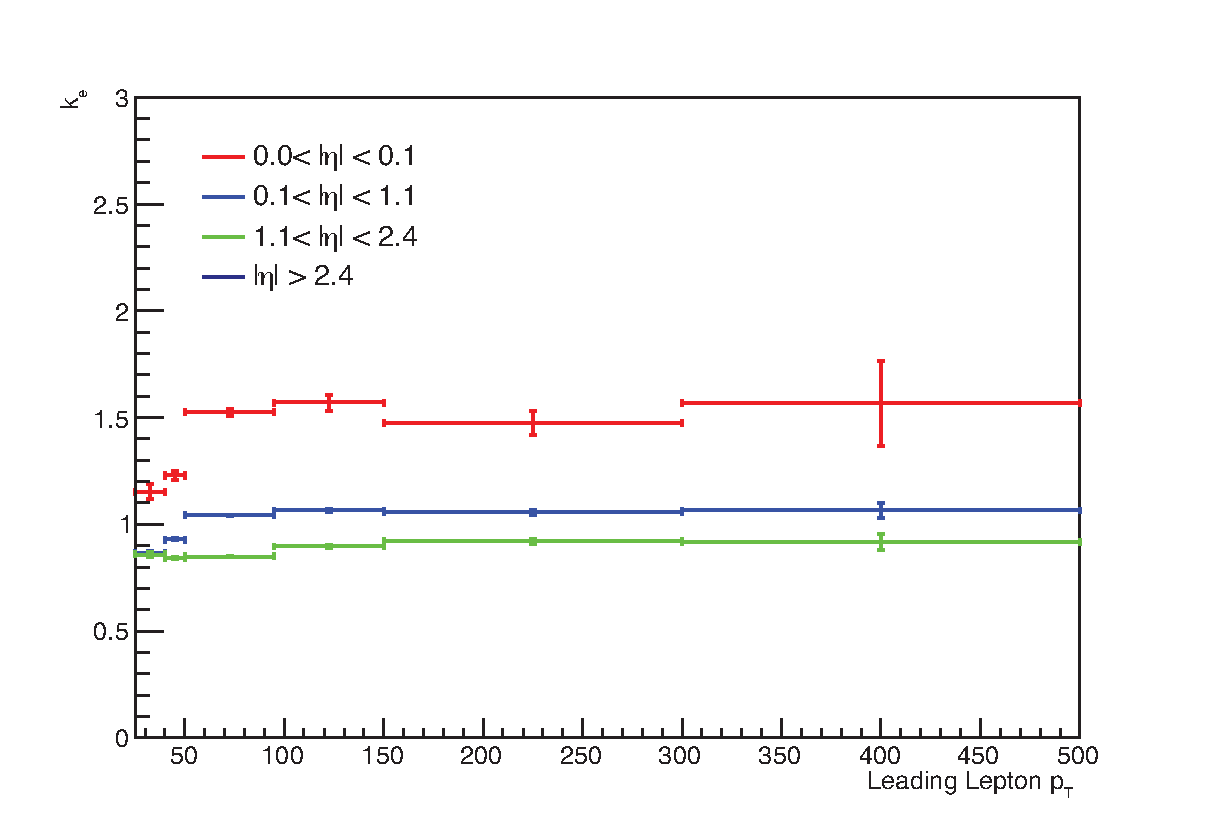
\includegraphics[width=.85\linewidth]{figures/fs/data_efficiencies_2j_Z_lep0.eps}
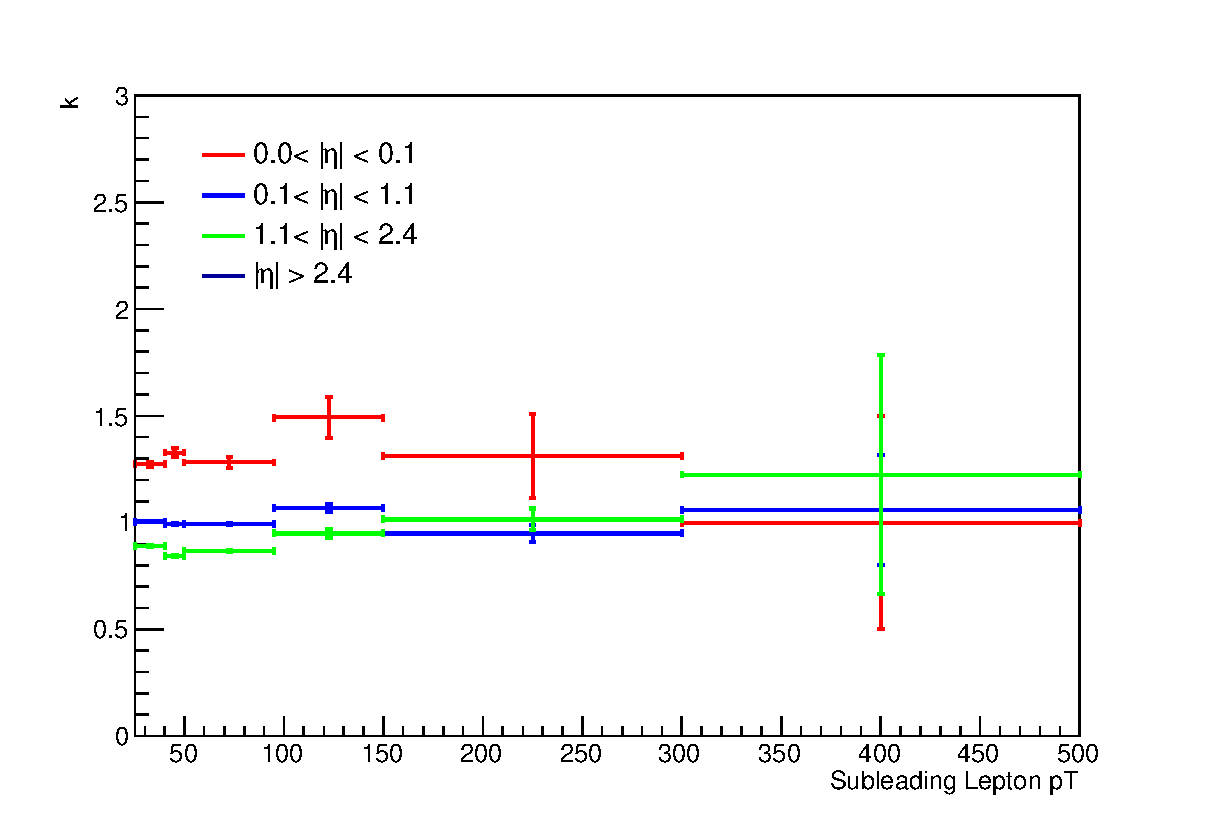
\includegraphics[width=.85\linewidth]{figures/fs/data_efficiencies_2j_Z_lep1.eps}
\caption{Measurements of $k_e$, the ratio of electron to muon events, in bins of $\pT$ and $\eta$, with statistical uncertainties shown. On the top is the measurements indexed by the leading lepton, while the measurements indexed by the subleading lepton are on the bottom. The efficiencies displayed are for the 2016 dataset.}
\label{fig:fs_k}
\end{figure}
\end{centering}

The estimate is corrected for contamination of non-\ac{FS} backgrounds in CR-FS according to
%
\begin{equation}
f_{\mathrm{FS}} = \frac{N_\text{obs} - N_\text{non-FS}}{N_\text{obs}}
\end{equation}
%
where $N_\text{obs}$ is the number of observed data events in CR-FS, and $N_\text{non-FS}$ is the number of expected events in CR-FS not resulting from \ac{FS} processes. This number is taken from \ac{MC} for all backgrounds except for fakes, which are estimated using the data-driven matrix method described in \autoref{sec:bg-fake}. According to the estimate, fakes account for about 65\% of the contamination in this region, with the remaining contamination resulting from diboson (15\%) and rare top (20\%) processes. $f_{\mathrm{FS}}$ is about 95\% in CR-FS. 

The way this fraction is calculated, any backgrounds that are not accounted for in $N_\text{non-FS}$ would be assumed to be \ac{FS}. Instead, the \ac{MC} could be used to predict the number of events that are \ac{FS}, which would result in any unaccounted for backgrounds being identified as non-\ac{FS}. The former procedure is preferable for several reasons. First, it reduces the dependence on \ac{FS} \ac{MC}, which is important for maintaining this method's independence from the Sideband Fit cross-check method discussed in \autoref{sec:method-sideband}. It also provides a conservative estimate of the number of \ac{FS} events, making an underestimate of the background less likely. Lastly, if for example, the number of fakes were underestimated, $f_{\mathrm{FS}}$ would increase, partially compensating for the underestimate.  

A prediction is made both for SRZ using the 91 events measured in CR-FS, and the lower-\met validation region, VRS, with the 277 events in VR-FS. The background estimation is performed separately for the two data taking periods, 2015 and 2016, because of the changing triggers and conditions. The results are then summed together, as shown in \autoref{tab:fs_yields}. The uncertainties in this table are discussed in \autoref{sec:unc_fs}.

\begin{table}
\begin{center}
 \begin{tabular}{lccc}
   \hline 
   Region & $ee$ prediction & $\mu\mu$ prediction & combined prediction \\
   \hline
   \hline
   %\multicolumn{4}{c}{Prediction for 14.7~\ifb\ of 2015+2016 Data} \\
   %\hline
SRZ & $ 16.5 \pm 2.1 $ & $ 16.7 \pm 2.0 $ & $ 33.2 \pm 3.9 $ \\
VRS & $ 49.7 \pm 4.6 $ & $ 49.6 \pm 4.6 $ & $ 99.3 \pm 8.5 $ \\
\hline
\hline
 \end{tabular}
\end{center}
 \caption{
   Yields in signal and validation regions for the flavor symmetric background. Errors include statistical and systematic uncertainties, discussed in \autoref{ch:background_uncertainties}. }
 \label{tab:fs_yields}
\end{table}

\subsection{Sideband Fit Method}
\label{sec:method-sideband}

As a crosscheck to the flavor symmetry method, a \ac{MC}-based method is used. This method is called a \textit{sideband fit}, and it begins with a \ac{MC} estimate of the signal region across an \mll~range that includes all values above 40 \gev. This region, excluding the on-$Z$ range that makes up the \ac{SR}, is used as a control region, defined as CRT in \autoref{tab:regions-z}. 

The \ac{SM} backgrounds are estimated for CRT using \ac{MC}, except for the fakes background, which is taken from the data-driven method described in \autoref{sec:bg-fake}. This background prediction is then fit to the measured data yield in CRT with one free parameter, $\mu$. This parameter scales the overall normalization of \ttbar \ac{MC}. All other backgrounds contributing to this control region are constrained by their uncertainties, which are used as nuisance parameters in the fit. Once $\mu$ has been acquired from this fit, it is applied to the \ttbar \ac{MC} yield in the \ac{SR}. This scaled \ttbar \ac{MC} is added to the raw \ac{MC} estimates of the other \ac{FS} processes to give a final estimate of the \ac{FS} background. 

The results of the fit can be seen in \autoref{tab:Yields_sideband_mc}, along with the original \ac{MC} or data-driven estimates for each background. The bottom half of the table shows the raw \ac{MC} estimates, as well as data-driven estimates for the fakes and \dyjets backgrounds. The top half of the table shows values for each of these quantities after the fit. The only significant change after the fit is the \ttbar background, which is scaled with $\mu$ = 0.64. Normalization factors acquired in CRT, including $\mu$ and the nuisance parameters for other \ac{MC}-driven backgrounds, are applied to SRZ. 



\begin{sidewaystable*}
\begin{center}
\setlength{\tabcolsep}{0.0pc}
{\small
%%
\begin{tabular*}{\textwidth}{@{\extracolsep{\fill}}lrrrr}
\noalign{\smallskip}\hline\noalign{\smallskip}
{\bf  channel}           & $ee/\mu\mu$ CRT            & $ee/\mu\mu$ SRZ            & $ee$ SRZ            & $\mu\mu$ SRZ              \\[-0.05cm]
\noalign{\smallskip}\hline\noalign{\smallskip}
%%
Observed events          & $273$              & $60$              & $35$              & $25$                    \\
\noalign{\smallskip}\hline\noalign{\smallskip}
%%
Fitted bkg events         & $272.76 \pm 16.88$          & $49.33 \pm 8.04$          & $27.09 \pm 4.73$          & $22.70 \pm 3.80$              \\
\noalign{\smallskip}\hline\noalign{\smallskip}
%%
        Fitted flavour symmetry events         & $236.96 \pm 21.66$          & $28.96 \pm 7.47$          & $16.41 \pm 4.33$          & $12.55 \pm 3.29$              \\
%%
        Fitted $WZ/ZZ$ events         & $4.03 \pm 1.13$          & $14.27 \pm 4.45$          & $7.81 \pm 2.45$          & $6.46 \pm 2.07$              \\
%%
        Fitted {\sc Sherpa} \dyjets\ events         & $1.95 \pm 0.14$          & --          & --          & --              \\
%%
        Data-driven \dyjets (\gjets) events         & --          & $3.10 \pm 2.25$          & $1.02_{-1.02}^{+1.25}$          & $2.08 \pm 1.38$              \\
%%
        Fitted rare top events         & $4.04 \pm 1.04$          & $2.90 \pm 0.76$          & $1.39 \pm 0.38$          & $1.50 \pm 0.40$              \\
%%
        Data-driven fake lepton events         & $25.78 \pm 14.26$          & $0.10_{-0.10}^{+0.18}$          & $0.46 \pm 0.45$          & $0.10 \pm 0.01$              \\
%%     
 \noalign{\smallskip}\hline\noalign{\smallskip}
%%
Expected \ac{SM} Events              & $366.71$          & $61.01$          & $33.73$          & $27.74$              \\
\noalign{\smallskip}\hline\noalign{\smallskip}
%%
        MC flavour symmetry events         & $331.32$          & $40.72$          & $23.09$          & $17.63$              \\
%%
        MC $WZ/ZZ$ events         & $4.02$          & $14.20$          & $7.77$          & $6.43$              \\
%%
        MC {\sc Sherpa} \dyjets\ events         & $1.94$          & --          & --          & --              \\
%%
        Data-driven \dyjets (\gjets) events         & --          & $3.10$          & $1.02$          & $2.08$              \\
%%
        MC rare top events         & $4.04$          & $2.89$          & $1.39$          & $1.50$              \\
%%
        Data-driven fake lepton events         & $25.39$          & $0.10$          & $0.46$          & $0.10$              \\
%%     \\
\noalign{\smallskip}\hline\noalign{\smallskip}
\end{tabular*}
%%%
}
\end{center}
\caption{
Background fit results from the sideband fit method. The \ttbar \ac{MC}'s normalization is taken as a free parameter in the fit to data in CRT, then that normalization factor is applied in SRZ. The results are shown here both divided between the $ee$ and $\mu\mu$ channels and summed together. All other backgrounds are taken from \ac{MC} in CRT, while in SRZ, the \dyjets contribution is taken from the \gjets method. The uncertainties quoted include both statistical and systematic components.}

\label{tab:Yields_sideband_mc}\end{sidewaystable*}
%


To validate the method, it is repeated in VRS using a fit acquired from VRT. These regions are identical to SRZ and CRT, but with \met ranging from 100 to 200 \gev. The normalization factors, listed in \autoref{tab:muTop}, are significantly different for the two regions. This difference is expected because the \ttbar \ac{MC} over-predicts the high-\met tail. This discrepancy between data and \ac{MC} is likely due to a mismodeling of of the top quark \pt distribution, which does not match the spectrum seen in data \cite{Aad:2015hna,Khachatryan:2016gxp}. \autoref{fig:fs_mc_met} shows the lepton \pt distribution in \ttbar events, demonstrating this discrepancy. This sideband fit method corrects for this mismodeling by performing fits in regions very kinematically similar to the signal region. 

\begin{table}[hbt]
\begin{center}
\begin{tabular}{lc}
\hline
Fit region & \ttbar\ normalization ($\mu$) \\ 
\hline\hline
CRT & $0.64 \pm 0.18$ \\
VRT & $0.80 \pm 0.09$ \\
\hline
\hline
\end{tabular}
\caption{
Summary of the \ttbar\ normalization factors calculated by the sideband fit to CRT and VRT for the 2015+2016 data. 
}
\label{tab:muTop}
\end{center}
\end{table}

\begin{centering}
\begin{figure}[!hbt]
\myfloatalign
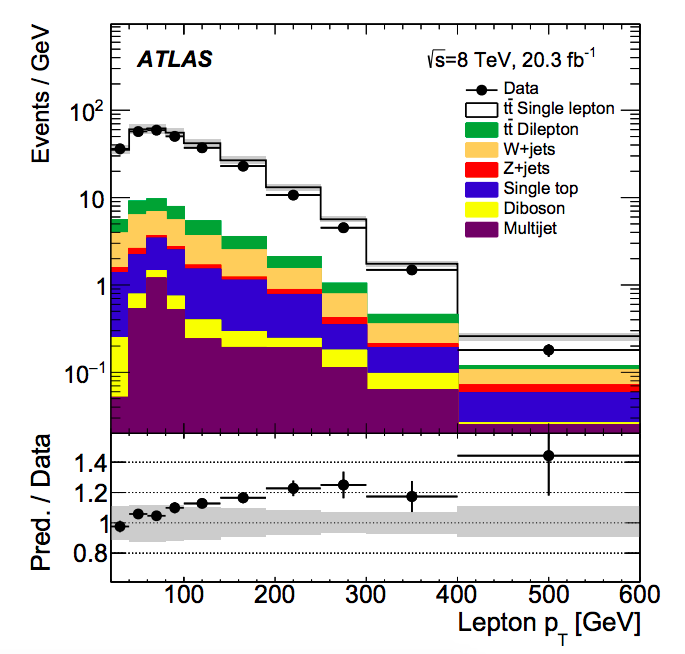
\includegraphics[width=.85\linewidth]{figures/fs/ttbar_mismodeling.png}
\caption{Lepton \pt distribution in data and \ac{MC}, demonstrating the overestimate of the high-\pt tail in \ac{MC} \cite{Aad:2015hna}.}
\label{fig:fs_mc_met}
\end{figure}
\end{centering}

This method is extremely effective as a crosscheck because it uses a completely independent dataset from the flavor symmetry method, and the two methods have very little overlap in dependence on \ac{MC}. If a misunderstanding of the background composition of CR-FS were to occur, it could alter the Flavor Symmetry prediction, but the Sideband Fit method should be unaffected. If the \ac{MC} shape of \ttbar were significantly mismodeled across the large \mll~range used in the Sideband Fit, this could yield a poor prediction, but the Flavor Symmetry method only uses the shape from \ac{MC} in a narrow band around the $Z$ peak, so it would be largely insensitive to this mismodeling. The two methods produce consistent results in both SRZ and VRS, as shown in \autoref{tab:fs_comparison}, demonstrating that significant mismodelings of either of these features is unlikely.


\begin{table}[h]
\centering

\begin{tabular}{ccc}
\noalign{\smallskip}\hline\noalign{\smallskip}
Region  & Flavour-symmetry  & Sideband fit  \\
\noalign{\smallskip}\hline\hline\noalign{\smallskip}
SRZ & $33 \pm 4$   &  $29 \pm 7$  \\ [+0.05cm]
VRS & $99\pm8$        &  $92 \pm 25$  \\ [+0.05cm]
\noalign{\smallskip}\hline\hline
\end{tabular}
\caption{ Comparison of \ac{FS} background predictions from the nominal method, the flavor symmetry method, and the cross-check, the sideband fit method. Uncertainties include statistical and systematic uncertainties in both cases. }
\label{tab:fs_comparison}
\end{table}

%-------------------------------------------------------------------------------------

\section{\dyjets Background}
\label{sec:bg-z}

The \dyjets background is produced by a process called Drell-Yan in which annihilating quark/anti-quark pairs produce a $Z$ boson or a virtual photon. These bosons then decay to two leptons, which, in the case of the $Z$ boson, naturally appear in the $Z$-mass window. This process can occur in association with jets due to initial state radiation, which can satisfy the jet and \HT requirements in SRZ. However, this process rarely produces real \met (though occasionally neutrinos do appear in hadronic decays of a $Z$ boson), so most events with large amounts of \met are the result of mismeasurement \footnote{$Z\rightarrow\tau\tau$ events do produce real \met, but these decays are grouped into the \ac{FS} background, and are not considered here.}. The 225 \gev~\met cut in SRZ includes $Z$ events only from the very high tail of the \met distribution, so a small mismodeling of jet resolution or energy scale in \ac{MC} can drastically change the prediction. If the prediction of the \dyjets background is too low, this will result in a signal-like peak of data over expected background. 

Because of the sensitivity to mismodeling in the \ac{MC} prediction of these high \met tails, a data-driven method is used to estimate this background. The method uses \gjets events which, like the \dyjets events, contain one boson recoiling against a hadronic system. These \gjets events are then corrected for the kinematic differences between photons and $Z$ bosons \cite{ATLAS:2012ema, Chatrchyan:2012qka}. The sample of \gjets events is taken from CR-$\gamma$, defined in \autoref{tab:regions-z}. This region is similar to the SRZ selection without the \met  requirement, but it vetoes events with leptons and requires at least one photon. Additionally, the $\Delta\phi(\text{jet}_{12},{\boldsymbol p}_{\mathrm{T}}^\mathrm{miss})$ cut in SRZ, which is designed to reduce the background from mismeasured jets, is removed for this region because of its unpredictability at very low values of \met, when the angle of the \met is much less meaningful. 

Despite their similarities, there are many theoretical differences between $\gamma$ and $Z$ events. The massive $Z$ boson requires more energy to produce than the massless photon, producing a difference in the kinematic distributions for bosons and jets in these events. Another consequence of photon's masslessness is that they must be produced with associated jets; otherwise, the process cannot simultaneously satisfy conservation of energy and momentum. As a consequence of these differences, many kinematic variables have different shapes between the two samples. \autoref{fig:photon_ptdist} shows a \ac{MC} comparison of boson \pt between $\gamma$ and $Z$ events, demonstrating the shape differences between the two processes. 

\begin{centering}
\begin{figure}[!hbt]
\myfloatalign
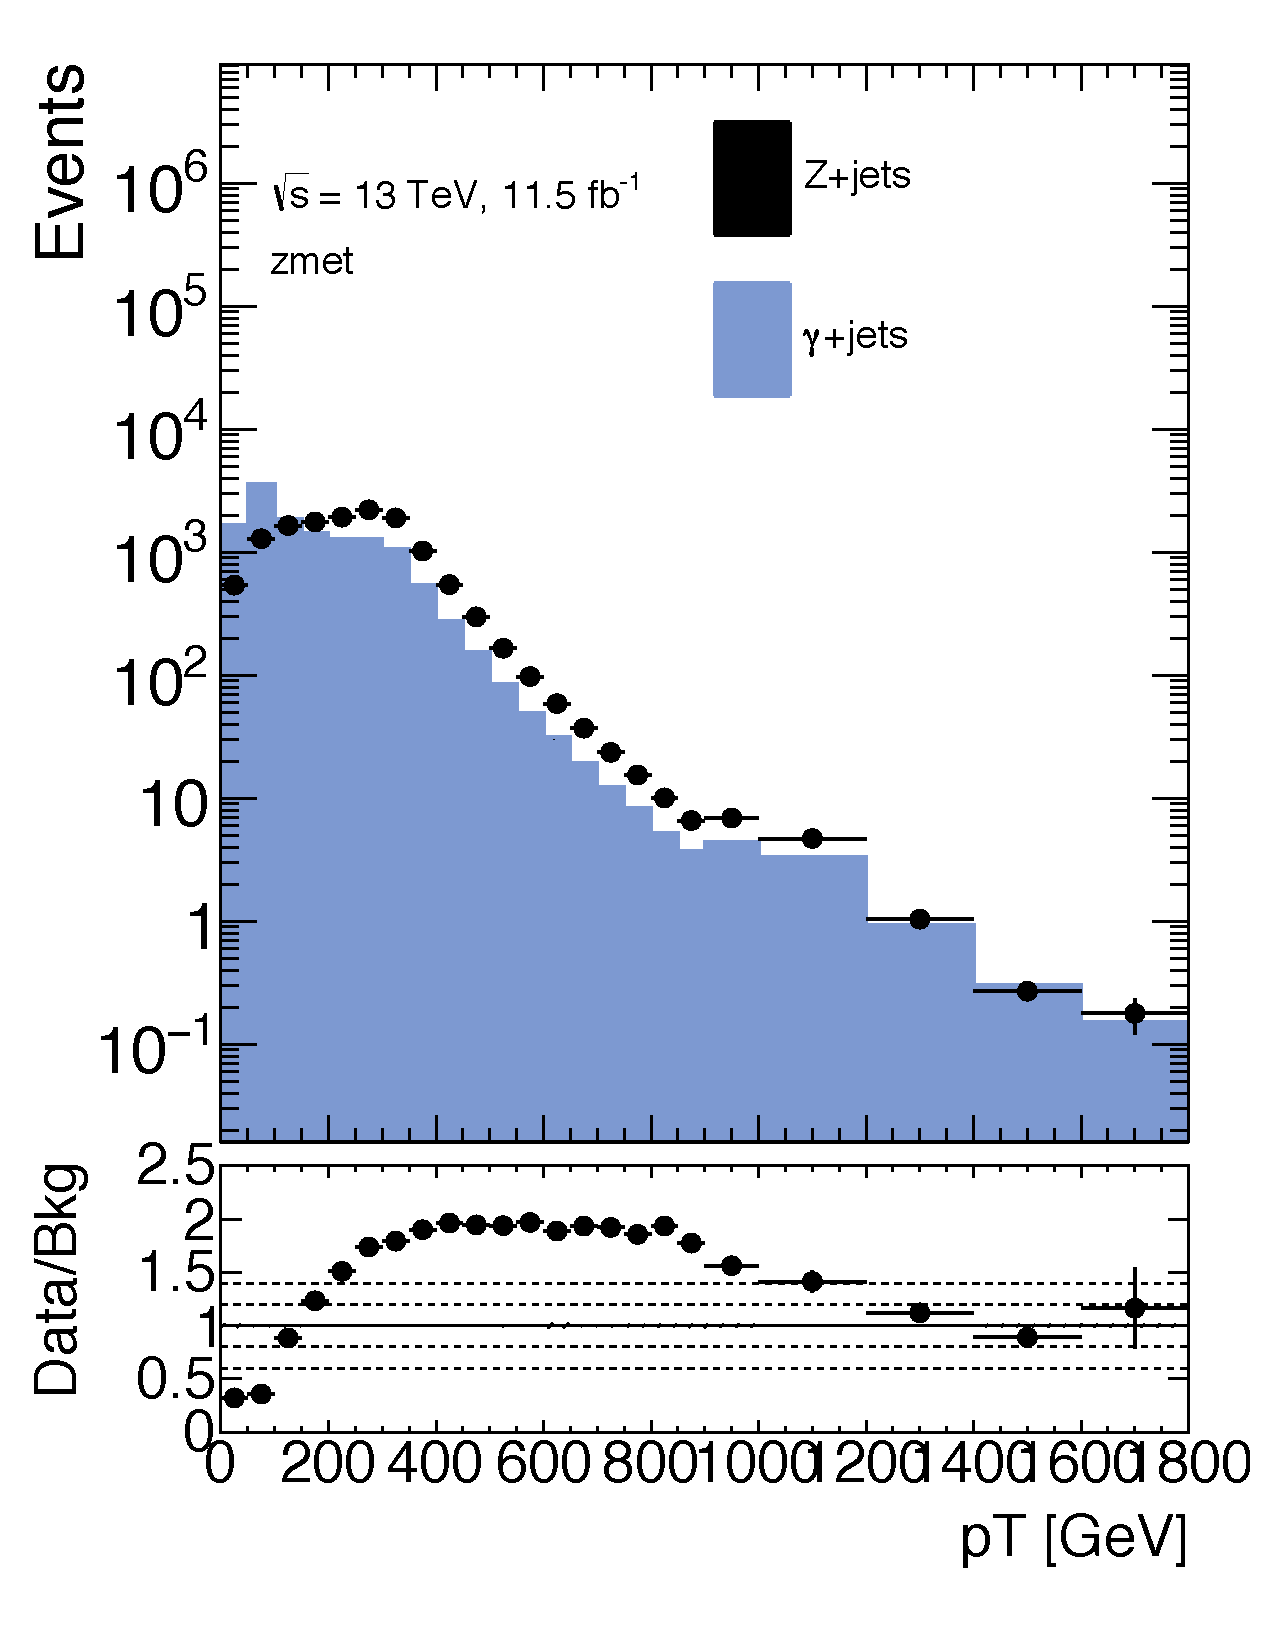
\includegraphics[width=.85\linewidth]{figures/photons/MC_hist_pt_0_SF_2j_2016_mcmetl___zmet_edit.pdf}
\caption{\ac{MC} comparison of boson \pt in a selection of photon and $Z\rightarrow\ell\ell$ events with \HT > 600 \gev. The feature at 1000 \gev~is not physical, but a reflection of the change in bin size. }
\label{fig:photon_ptdist}
\end{figure}
\end{centering}

The most significant experimental difference between $Z$ and $\gamma$ events is that $Z$ bosons rapidly decay, in the case of this analysis, to two leptons, which are then be observed by the \ac{ATLAS} detector. In contrast, the photon is stable, and can be directly detected by \ac{ATLAS}. This means that the reconstructed $Z$ boson has an energy resolution that's the convolution of the resolutions of either a pair of electrons or a pair of muons, while the photon resolution is the result of only one measurement. Though electron and photon resolutions are similar because both depend on the electromagnetic calorimeter, the difference between the measurement of two, lower-\pt objects and one higher-\pt object creates small differences. The muons, whose energy measurements rely on the reconstruction of tracks in the \ac{ID} and \ac{MS}, have a very different momentum resolution from either electrons or photons. 

In addition, this difference in detection means there is a minimum value for the \pt of the photons observed; only photons with \pt > 35 \gev~are consistently identified by the trigger. For the $Z$ boson, there is no direct minimum on \pt, only a reduction of efficiency at low values due to the minimum \pt values of the leptons used to reconstruct them. 

The goal of this method is to predict the \met distribution of the \dyjets background using a manipulated \gjets sample from data. These differences between $Z$+jet and $\gamma$+jet events can be broken down into two categories: differences which affect the jet energy and measurement, and differences which affect the boson energy and measurement. The differences in the hadronic system are simpler, and mostly consist of different numbers and energies of jets between the two samples, which can be accounted for via reweighting in a variable that is representative of the total energy scale of the event. The differences in the bosons are more complex, and require the application of smearing functions based on the different observed objects. Together these corrections allow for complete modeling of the \dyjets \met spectrum with $\gamma$+jet events.

% A $\Delta\phi$(\MET,jet) cut is applied in all SRs and VRs,
% but enforcing this on the \gjets\ (and \dyjets) data or MC samples from the beginning of this procedure can result in poorly modelled/truncated angular distributions later.
% The application of this kinematic cut is handled as follows:
% \begin{itemize}
% \item An SR-like selection is made with the same \HT\ cuts (or \htincl\ in the case of SRZ) and jet multiplicity cuts, but no $Z$-window selection (for SRZ), 
% no \met\ selection and no $\Delta\phi$(\MET,jet) cut.
% \item First, the photon \pt\ is smeared to better represent the resolution of a $Z$ boson decaying to either electrons or muons. 
% These smearing factors are derived in a 1-jet CR with identical kinematic requirements to those outlined above, but with exactly one jet.
% \item Second, the photon \pt\ is reweighted to match the $Z$ boson \pt\ distribution. 
% These reweighting factors are derived separately for each \HT\ or \htincl\ region.
% \item Third, the $\Delta\phi$(\MET,jet) cut is applied.
% \item Fourth, $V\gamma$ backgrounds are subtracted from the photon data sample so as to avoid contaminating the \dyjets estimate.
% \item Finally, the \mll\ cut is imposed on the \gjets\ data. 
% An \mll\ value is assigned to each photon according to the size of smearing that was applied to the photon and uses the \mll\ distribution from \dyjets\ MC.
% \end{itemize}

\subsection{Photon and $Z$ Event Selection}
\label{sec:photon_eventsel}

The baseline photon events come from CR-$\gamma$, an inclusive \ac{CR} with no \met cut, a lepton veto, and the requirement of at least one photon \footnote{This region includes an \HT cut, which requires the translation of photon \pt into an equivalent di-lepton \pt scalar sum. This process is described in \autoref{sec:photon_mll}.}. This selection is very pure in $\gamma$+jet events, but some $V\gamma$ events are also included, which can include real \met. These backgrounds are subtracted from the yield in this region according to \ac{MC}. The impact of these backgrounds and the process by which they are subtracted are discussed in \autoref{sec:gjets_vg}. 

The triggering scheme for these \gjets events is more complicated than in other regions because the lowest unprescaled photon trigger requires a photon \pt of at least 120 (140) \gev~ in 2015 (2016) datataking, but the method requires events with much lower \pt to predict the full $Z$-boson \pt spectrum. To accomplish this, the lower-\pt photons are collected with prescaled triggers with a designated trigger for each \pt range, listed in \autoref{tab:photon_triggers}. The events in each selection are then weighted by the prescale value of the trigger used to reconstruct a smooth \pt spectrum. 

\begin{table}[!hbt]
\centering
\begin{tabular}{lc}
\noalign{\smallskip}\hline\noalign{\smallskip}
\pt Range [\gev]  & Trigger Name  \\
\noalign{\smallskip}\hline\hline\noalign{\smallskip}
\multicolumn{2}{c}{2015 Data-Taking} \\
\noalign{\smallskip}\hline
$37<p_{\text{T}}<45$ 	& \texttt{HLT\_g35\_loose\_L1EM15} \\
$45<p_{\text{T}}<50$	& \texttt{HLT\_g40\_loose\_L1EM15} \\
$50<p_{\text{T}}<55$	& \texttt{HLT\_g45\_loose\_L1EM15} \\
$55<p_{\text{T}}<125$	& \texttt{HLT\_g50\_loose\_L1EM15} \\
$p_{\text{T}}>125$		& \texttt{HLT\_g120\_loose\_L1EM15} \\
\hline
\multicolumn{2}{c}{2016 Data-Taking} \\
\noalign{\smallskip}\hline
$25<p_{\text{T}}<30$ 	& \texttt{HLT\_g20\_loose\_L1EM12} \\
$30<p_{\text{T}}<40$ 	& \texttt{HLT\_g25\_loose\_L1EM12} \\
$40<p_{\text{T}}<45$ 	& \texttt{HLT\_g35\_loose\_L1EM12} \\
$45<p_{\text{T}}<50$ 	& \texttt{HLT\_g40\_loose\_L1EM12} \\
$50<p_{\text{T}}<55$ 	& \texttt{HLT\_g45\_loose\_L1EM12} \\
$55<p_{\text{T}}<65$ 	& \texttt{HLT\_g50\_loose\_L1EM12} \\
$65<p_{\text{T}}<75$ 	& \texttt{HLT\_g60\_loose\_L1EM12} \\
$75<p_{\text{T}}<85$ 	& \texttt{HLT\_g70\_loose\_L1EM12} \\
$85<p_{\text{T}}<105$ 	& \texttt{HLT\_g80\_loose\_L1EM12} \\
$105<p_{\text{T}}<145$ 	& \texttt{HLT\_g100\_loose\_L1EM12} \\
$p_{\text{T}}>145$ 		& \texttt{HLT\_g140\_loose\_L1EM12} \\
\noalign{\smallskip}\hline\hline
\end{tabular}
\caption{ List of triggers used to collect photon events in 2015 and 2016 data-taking.}
\label{tab:photon_triggers}
\end{table}

These $\gamma$ events can then be compared to baseline $Z\rightarrow\ell\ell$ events with a similar selection. These events have the same dilepton requirements as SRZ, without the \mll~cut. They also have no \met cut, but like the photons, are required to have \HT > 600 \gev~as in SRZ.  

\subsection{Smearing of Photon Events}
\label{sec:photon_smearing}

While $Z$+jet events are measured as a pair of leptons recoiling against a hadronic system, $\gamma$+jet events are measured only as one  object recoiling against jets. In addition, detector resolution is very different for muons and photons, though electrons and photons are similar. The impact of these differences must be corrected for in $\gamma$+jet events in order for them to accurately predict the \met distribution of the \dyjets events. In most cases, the resolution of the photon's \pt is better than that of the $Z$ boson, so the photon events can be smeared to emulate the $Z$ boson's resolution.  

To isolate mismeasurement of boson \pt, this method uses \metl, defined as
%
\begin{equation}
\metl = \met \mathrm{sin} \theta
\end{equation}
%
where $\theta$ is the angle between ${\boldsymbol p}_{\mathrm{T}}^\mathrm{miss}$ and the ${\boldsymbol p}_{\mathrm{T}}$ of the $Z$ boson. \autoref{fig:photon_metparallel} shows the \metl distribution in \ac{MC} for the two samples, and demonstrates the discrepancies between them. The core of the photon distribution is similar to the $Z\rightarrow ee$ distribution because measurements of both photons and electrons are primarily taken from the electromagnetic calorimeter and have the same resolution. For muons, which rely on tracks to determine \pt, the resolution becomes larger at high \pt values where the tracks are nearly straight. For a muon with a \pt of 200 \gev, this the resolution is about 5\%, while a photon or electron with the same \pt has a resolution of 1-2\% \cite{Aad:2014zya, Aad:2014nim}. As a consequence, the resolution distributions for photon and $Z\rightarrow\mu\mu$ events are very different. 

\begin{centering}
\begin{figure}[!hbt]
\myfloatalign
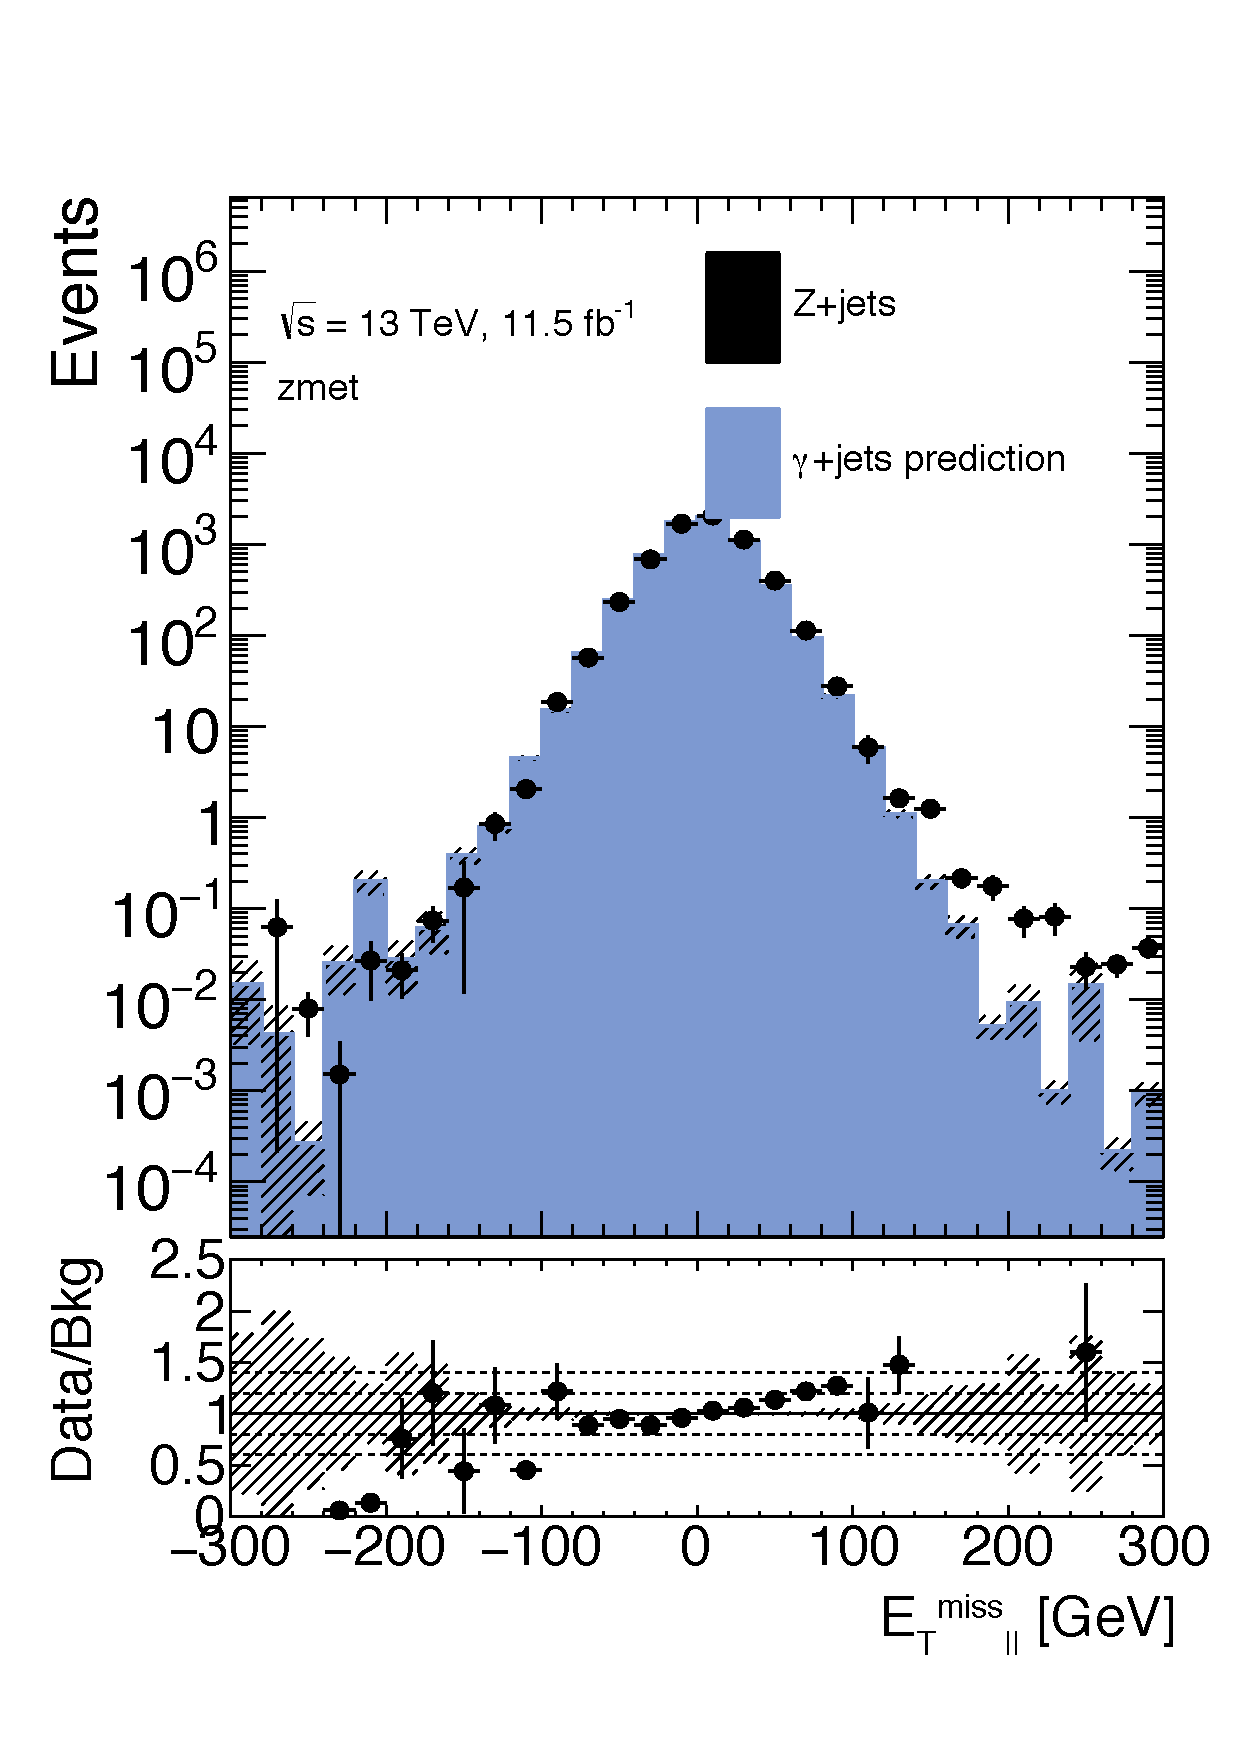
\includegraphics[width=.45\linewidth]{figures/photons/MC_hist_METl_Pt_0_ee_2j_2016_mcmetl_ptrw__zmet_.pdf}
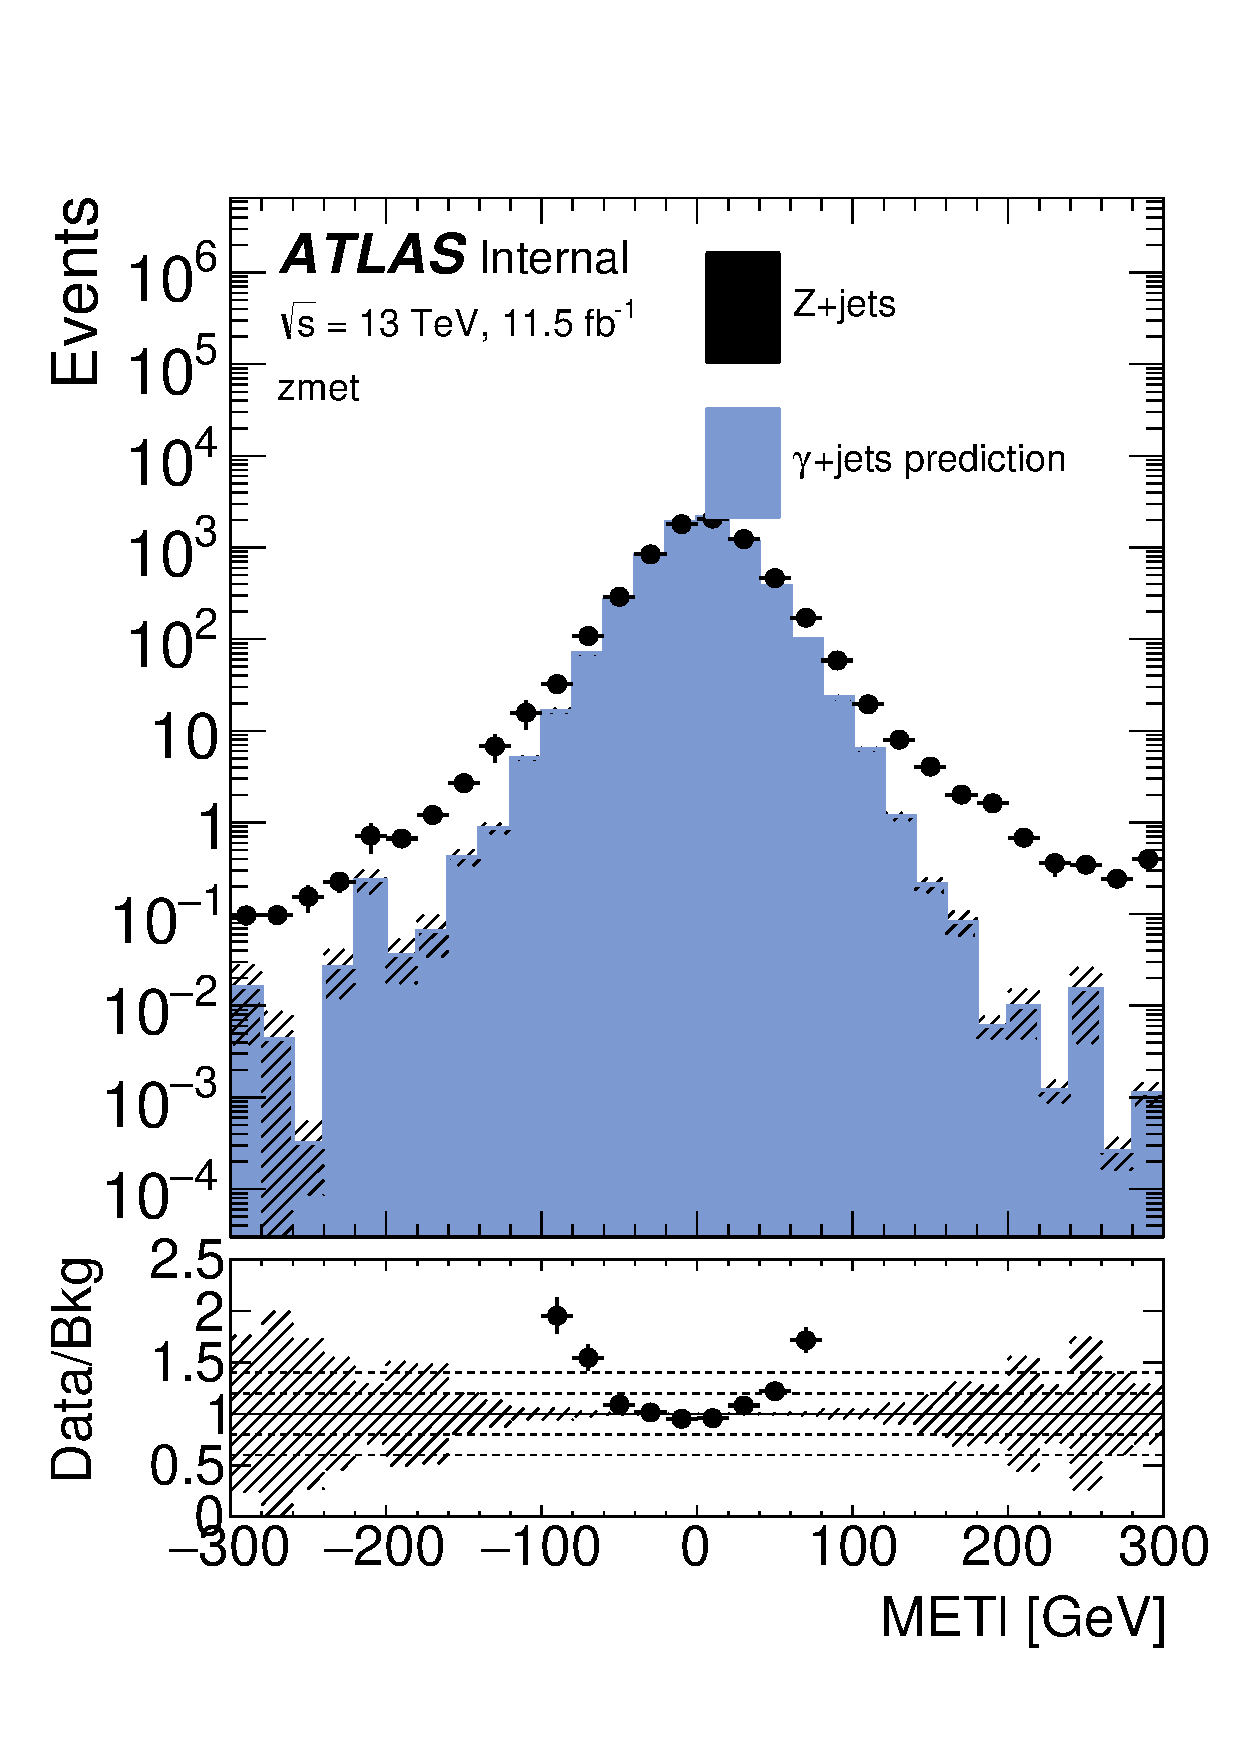
\includegraphics[width=.45\linewidth]{figures/photons/MC_hist_METl_Pt_0_mm_2j_2016_mcmetl_ptrw__zmet_.pdf}
\caption{\metl distributions in \ac{MC} for $Z$+jets in the $ee$ (left) and $\mu\mu$ (right) channels compared to the \gjets prediction in an inclusive region with \HT > 600 \gev.}
\label{fig:photon_metparallel}
\end{figure}
\end{centering}

A function to smear photon events is derived from the deconvolution of the \gjets and \dyjets \metl distributions, taken from 1-jet \acp{CR} with no \HT cut, which are otherwise identical to the baseline $Z$ and $\gamma$ selections. Assuming the jet response functions are the same for the two event types, the deconvolution should cancel these terms and leave a smearing function based only on the differences between photon and $Z$ boson resolutions. The 1-jet \acp{CR} are chosen both for the simplicity of the hadronic systems involved, and because they are orthogonal to the \ac{SR}.  
%This region is chosen because it is orthogonal to the \ac{SR}, so the resolution can be obtained from data as well as \ac{MC} without being affected by the . 

In these 1-jet \acp{CR}, events are first binned in boson \pt, and in each bin, a \metl distribution is made. The smearing function is defined for each bin as the deconvolution of the \dyjets and \gjets \metl distributions.
Next, for each photon event, the smearing function matching the event's photon \pt is sampled, yielding the smearing amount, $\Delta$\pt. The photon's \pt is then adjusted according to 
%
\begin{equation}
\pt^{\gamma\prime} = \pt^\gamma + \Delta\pt 
\end{equation} 
%
and the corresponding change in \met is made,
%
\begin{equation}
E_{T,\parallel}^{\text{miss}\prime} = \metl - \Delta\pt.
\end{equation}

The data- and \ac{MC}-derived smearing functions each have their own benefits. The data-based functions are of course not subject to any potential mismodeling, but it is possible to have contamination from other processes that is not accounted for. Because good agreement between data and \ac{MC} is seen in the \metl spectrums, contamination was deemed a higher concern than mismodeling, and the \ac{MC}-based function was used as the nominal smearing function, with the data-based function used as a cross-check.

The smeared \metl distributions can be seen in \autoref{fig:photon_metparallelsmeared}. Though there is a small amount of oversmearing in the negative tail, the improvement in agreement between the distributions, especially in their cores, is clear.

\begin{centering}
\begin{figure}[!hbt]
\myfloatalign
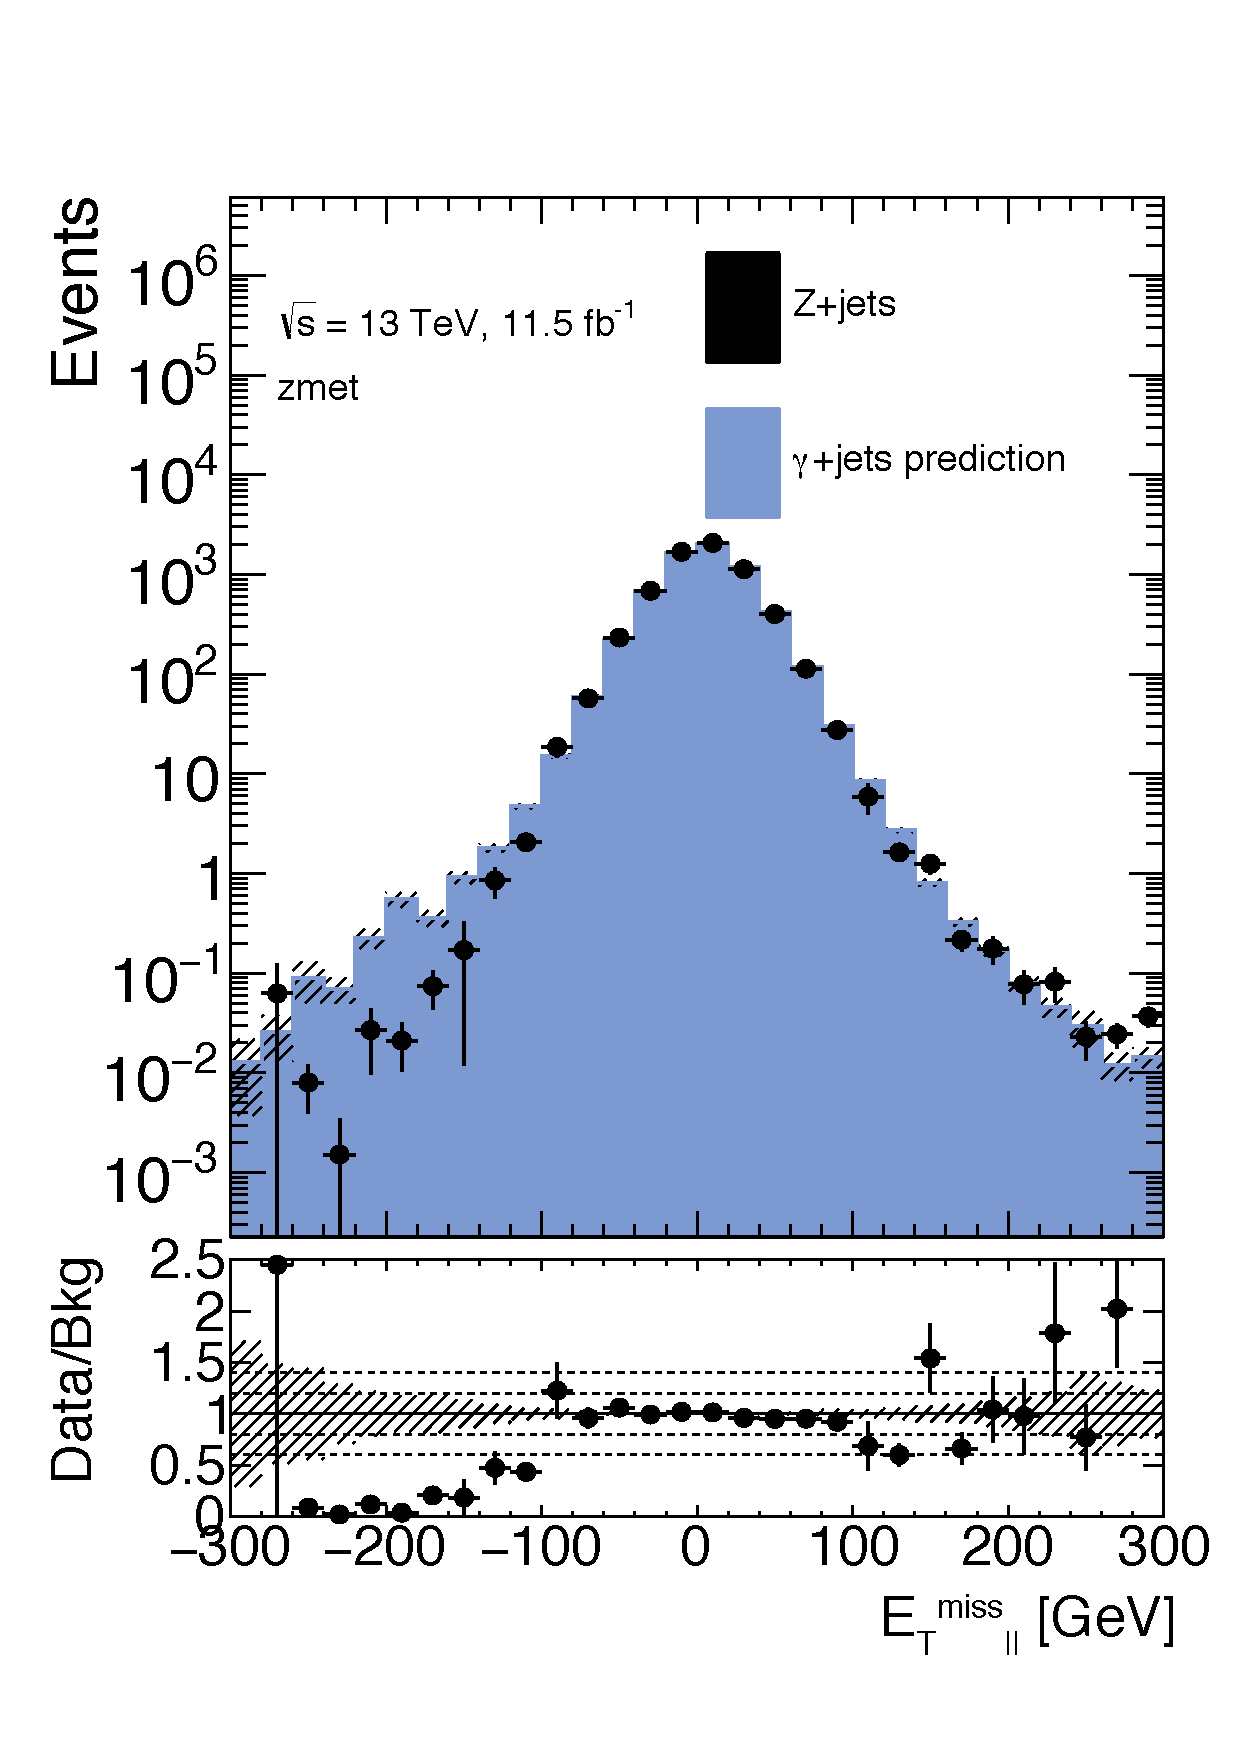
\includegraphics[width=.45\linewidth]{figures/photons/MC_hist_METl_Pt_0_ee_2j_2016_mcmetl_ptsmrw_smear_zmet_.pdf}
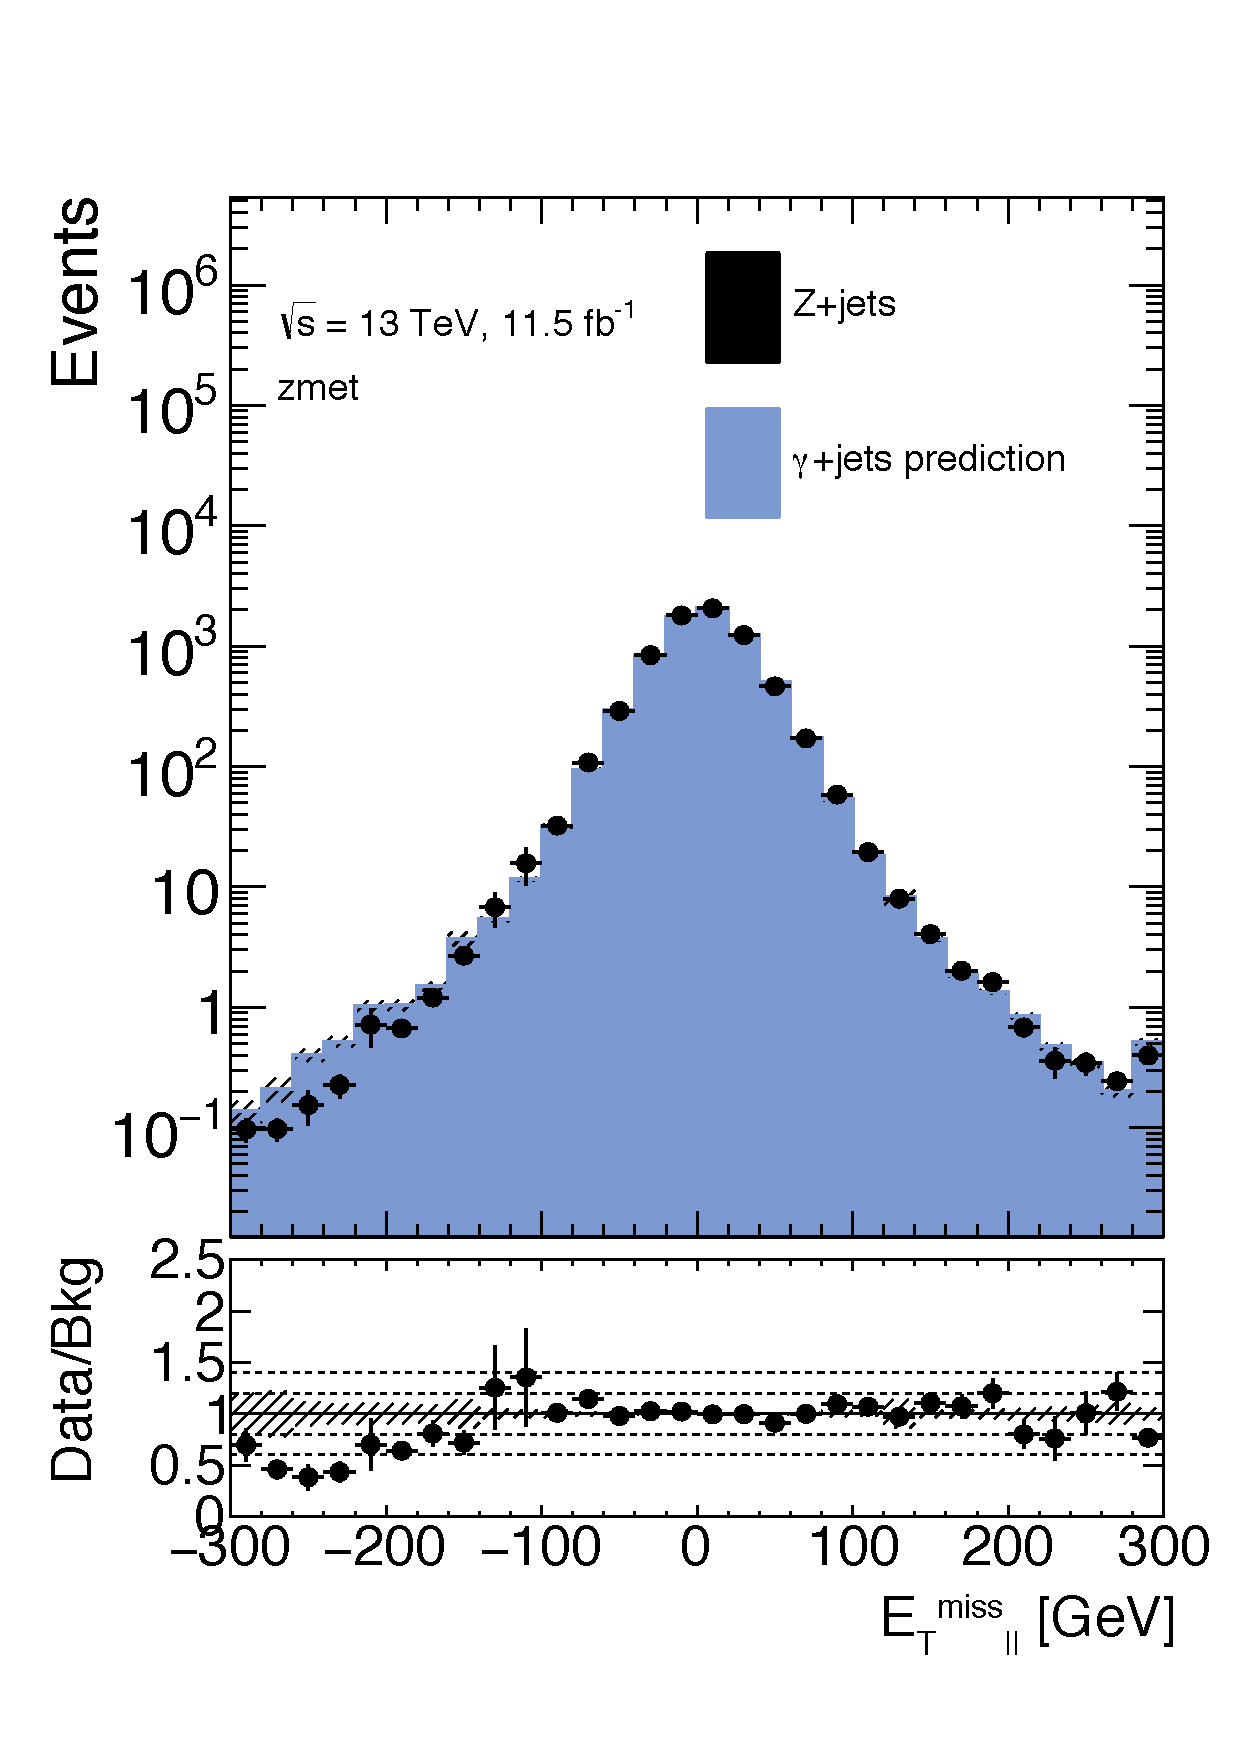
\includegraphics[width=.45\linewidth]{figures/photons/MC_hist_METl_Pt_0_mm_2j_2016_mcmetl_ptsmrw_smear_zmet_.pdf}
\caption{\metl distributions in \ac{MC} for $Z$+jets $ee$ (left) and $\mu\mu$ (right) channels compared to  \gjets in an inclusive region with \HT > 600 \gev after the smearing procedure has been performed. The events in these distributions have also been \pt reweighted, as described in \autoref{sec:photon_reweight}.}
\label{fig:photon_metparallelsmeared}
\end{figure}
\end{centering}

\subsection{\pt Reweighting of Photon Events}
\label{sec:photon_reweight}

Next, the photon events are reweighted to match the boson \pt spectrum of the $Z$ events. This is accomplished by making histograms of boson \pt for \gjets and \dyjets events with binning identical to the \pt bins used for the determination of smearing functions. Photons are binned based on their smeared \pt determined in the previous step. A reweighting factor $f(\pt)$ is then calculated in each bin, according to
%
\begin{equation}
f_\text{MC}(x) = \frac{N_{\dyjets}(x)}{N_{\gjets}(x)}
\end{equation}
%
in \ac{MC}, and in data according to
%
\begin{equation}
f_\text{data}(x) = \frac{N_{\text{data}}(x)-N_{t\bar{t}}(x)-N_{\text{VV}}(x)}{N_{\gjets\ \text{data}}(x)} ,
\end{equation}
%
where the contamination from other backgrounds is taken from \ac{MC} and subtracted from the $Z$ candidate sample. The resulting reweighting factors can be seen in \autoref{fig:photon_reweight} and are calculated independently for $ee$ and $\mu\mu$ events. The data-based reweighting function is used as the nominal function, while the \ac{MC}-based function is used for \ac{MC} closure tests described in \autoref{sec:unc_gjets}. 

\begin{centering}
\begin{figure}[!hbt]
\myfloatalign
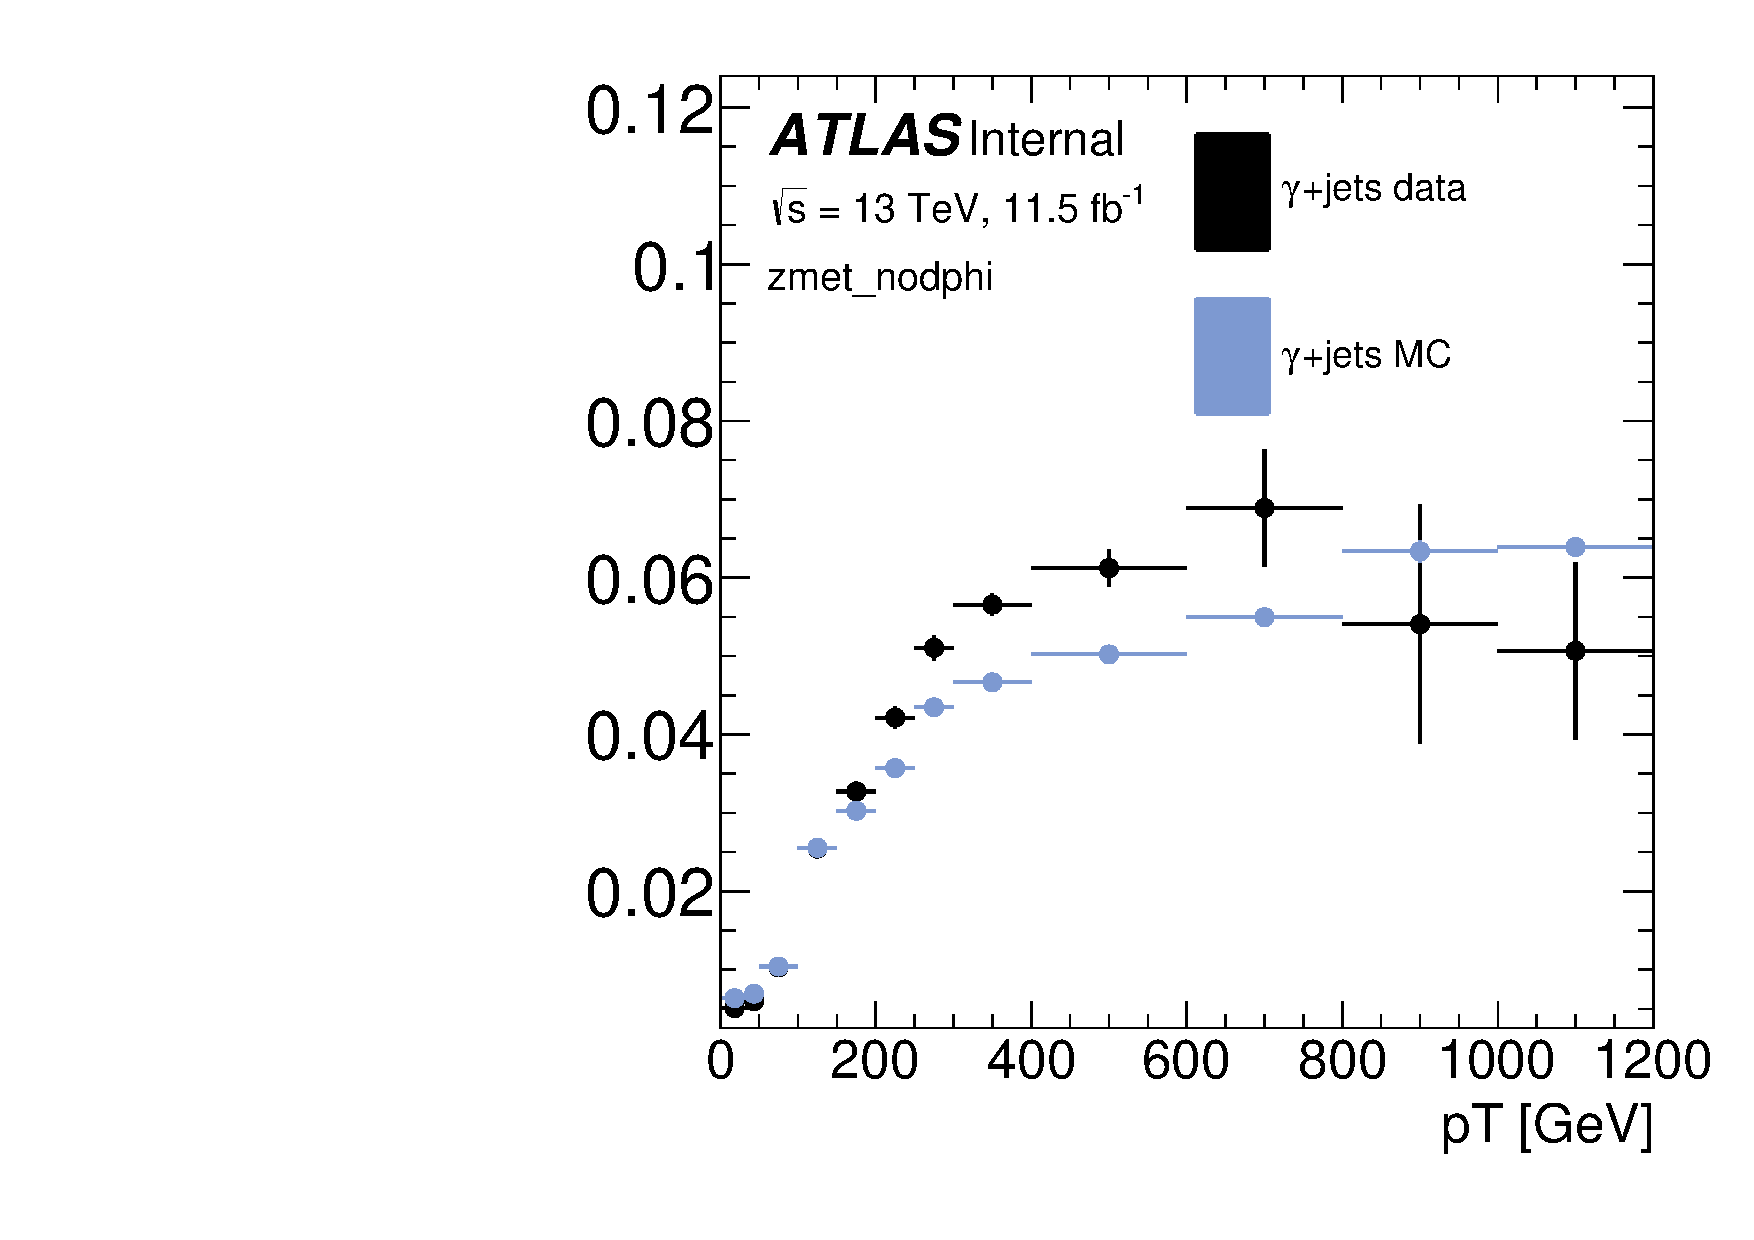
\includegraphics[width=.45\linewidth]{figures/photons/Corr_hist_ptrw_ee_2j_2016_mcmetl_ptsmrw_smear_zmet_nodphi_.pdf}
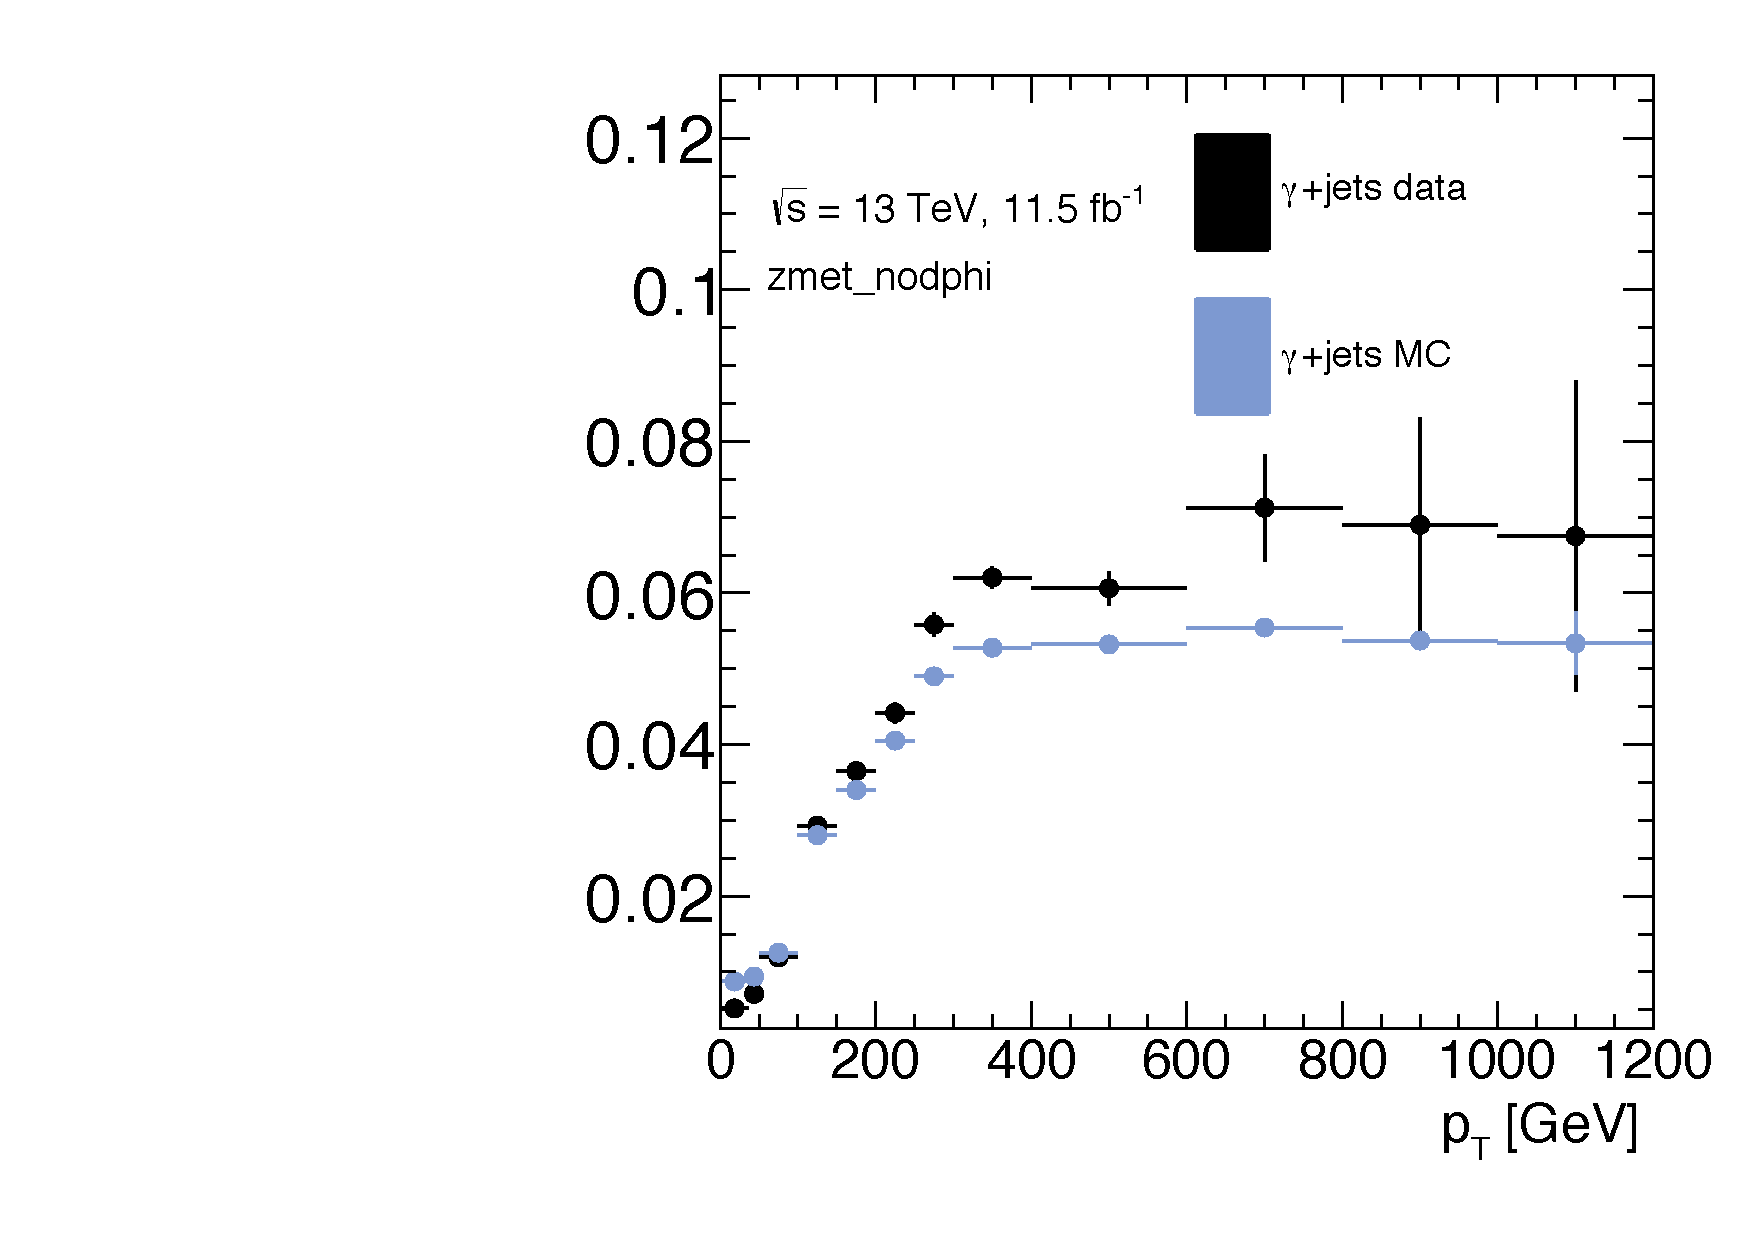
\includegraphics[width=.45\linewidth]{figures/photons/Corr_hist_ptrw_mm_2j_2016_mcmetl_ptsmrw_smear_zmet_nodphi_.pdf}
\caption{Photon reweighting factors for the $ee$ (left) and $\mu\mu$ (right) channels derived from data and \ac{MC}.}
\label{fig:photon_reweight}
\end{figure}
\end{centering}

This reweighting, though it is performed on the boson \pt, primarily serves to produce more similar jet distributions between the $\gamma$ and $Z$ samples. The boson \pt is serving here as a proxy for the energy scale of the event, and reweighting in this variable results in photon events with hadronic energy that approximately matches that of the \dyjets distributions. It is important to match the hadronic energy scales because the mismeasurement (and thus the \met) scales with the square of the observed hadronic energy. Other variables can be used for reweighting, and are used in the determination systematic uncertainties discussed in \autoref{sec:unc_gjets}, but boson \pt reweighting was observed to yield the best closure.

%Because, excluding \met contributions, the boson \pt must match the energy of the jet system off which it recoils, these two variables are closely tied. Once the two samples are reweighted to have similar amounts of hadronic energy, the \met contribution from mismeasurement of jets, which scales according to the square root of the jet energy, should also be the same between the two samples. 

Together, the boson smearing and \pt reweighting produce a \met spectrum in the modified photon events that closely matches that of the \dyjets events. Figures \ref{fig:photon_metchange_ee} and \ref{fig:photon_metchange_mm} show the comparison of the \met distributions before any alteration, with only \pt reweighting, and after the smearing and reweighting, demonstrating the impact of each step. In the $ee$ channel, the \met distribution looks similar between \dyjets and \gjets events up to about 150 \gev. Above this value, the differences between $\gamma$ and $Z\rightarrow ee$ resolutions seen in the tails of \autoref{fig:photon_metparallel} become significant. In the $\mu\mu$ channel, the discrepancy between the \met in \dyjets and \gjets events begins at much lower values. In both cases, the application of \pt reweighting and smearing result in excellent agreement between the two \met spectra, with most of the improvement resulting from the smearing factors. 

\begin{centering}
\begin{figure}[!hbt]
\myfloatalign
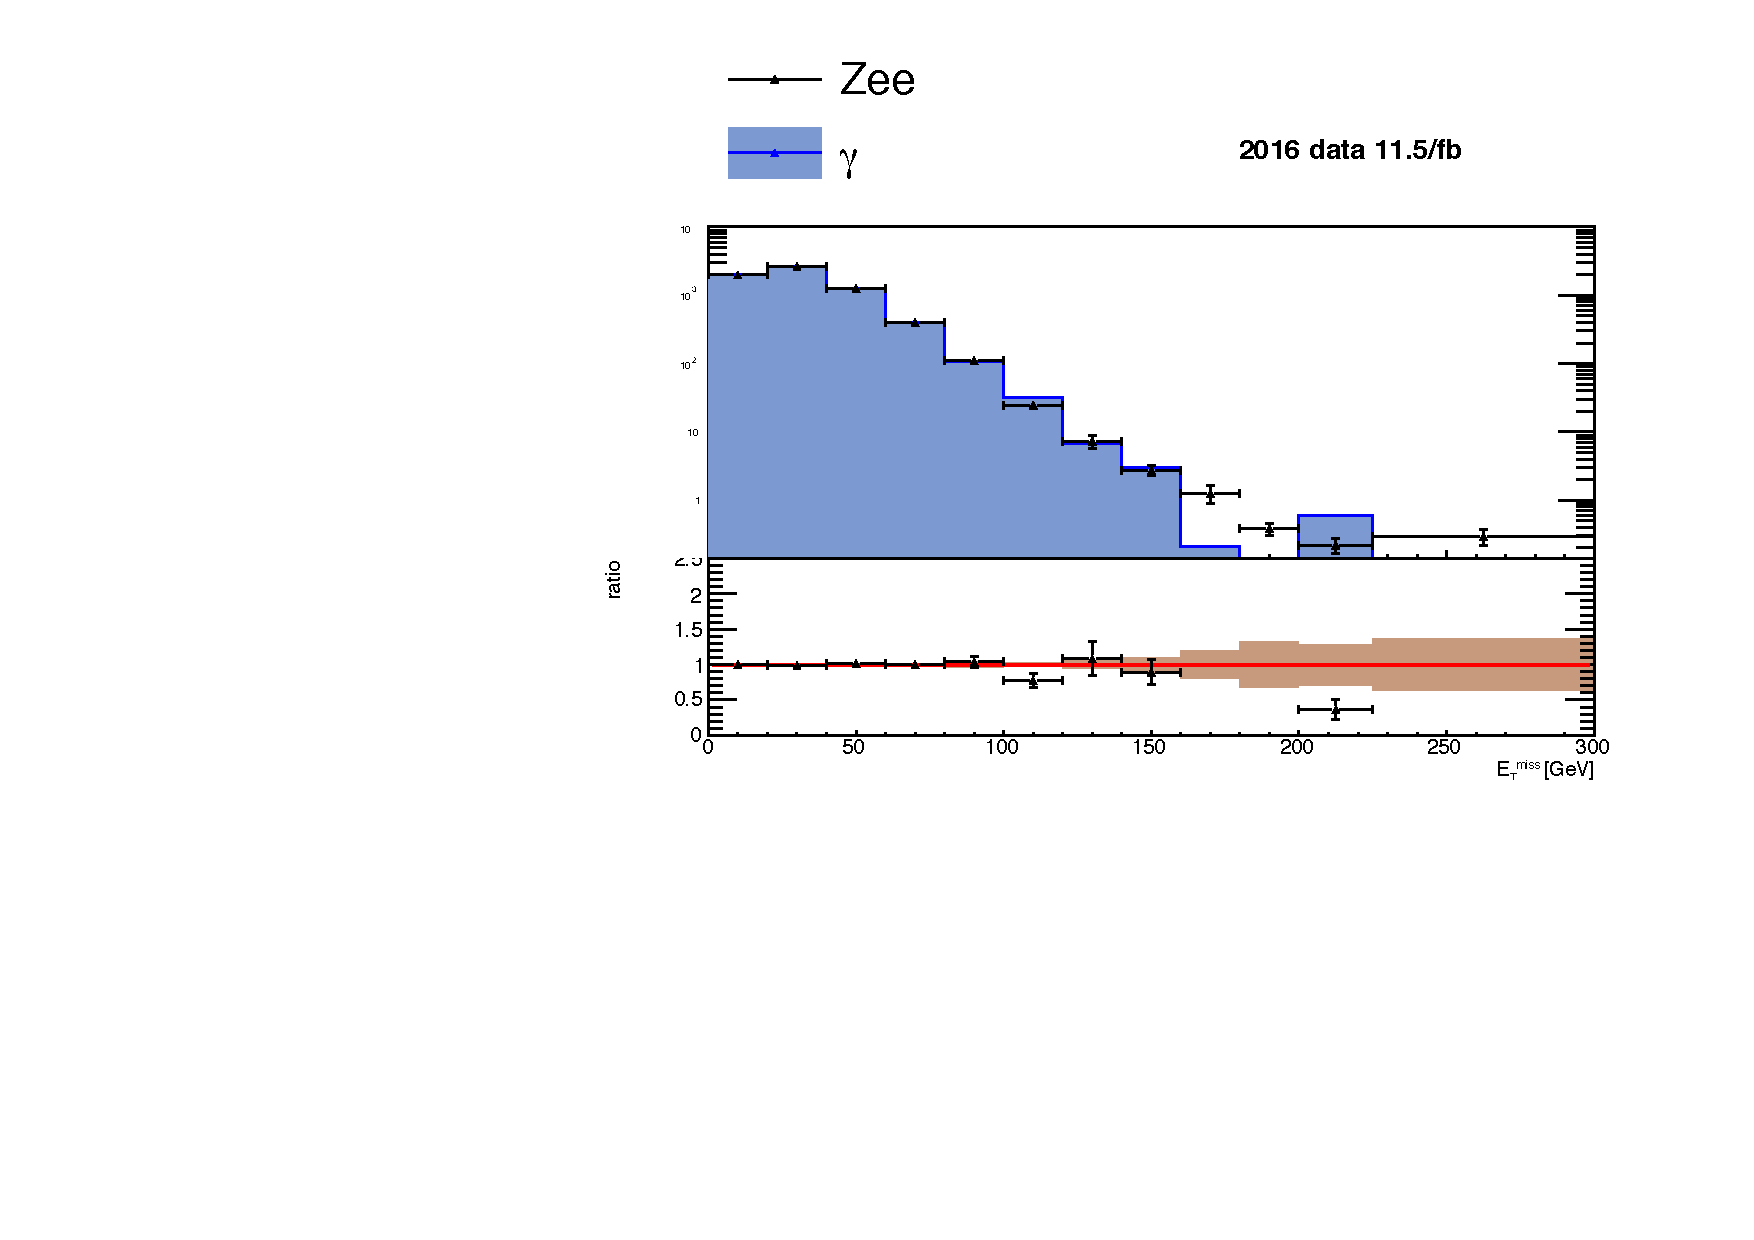
\includegraphics[width=.75\linewidth]{figures/photons/Photon_Zee_met_2j_2016_mcmetl___zmet.pdf}
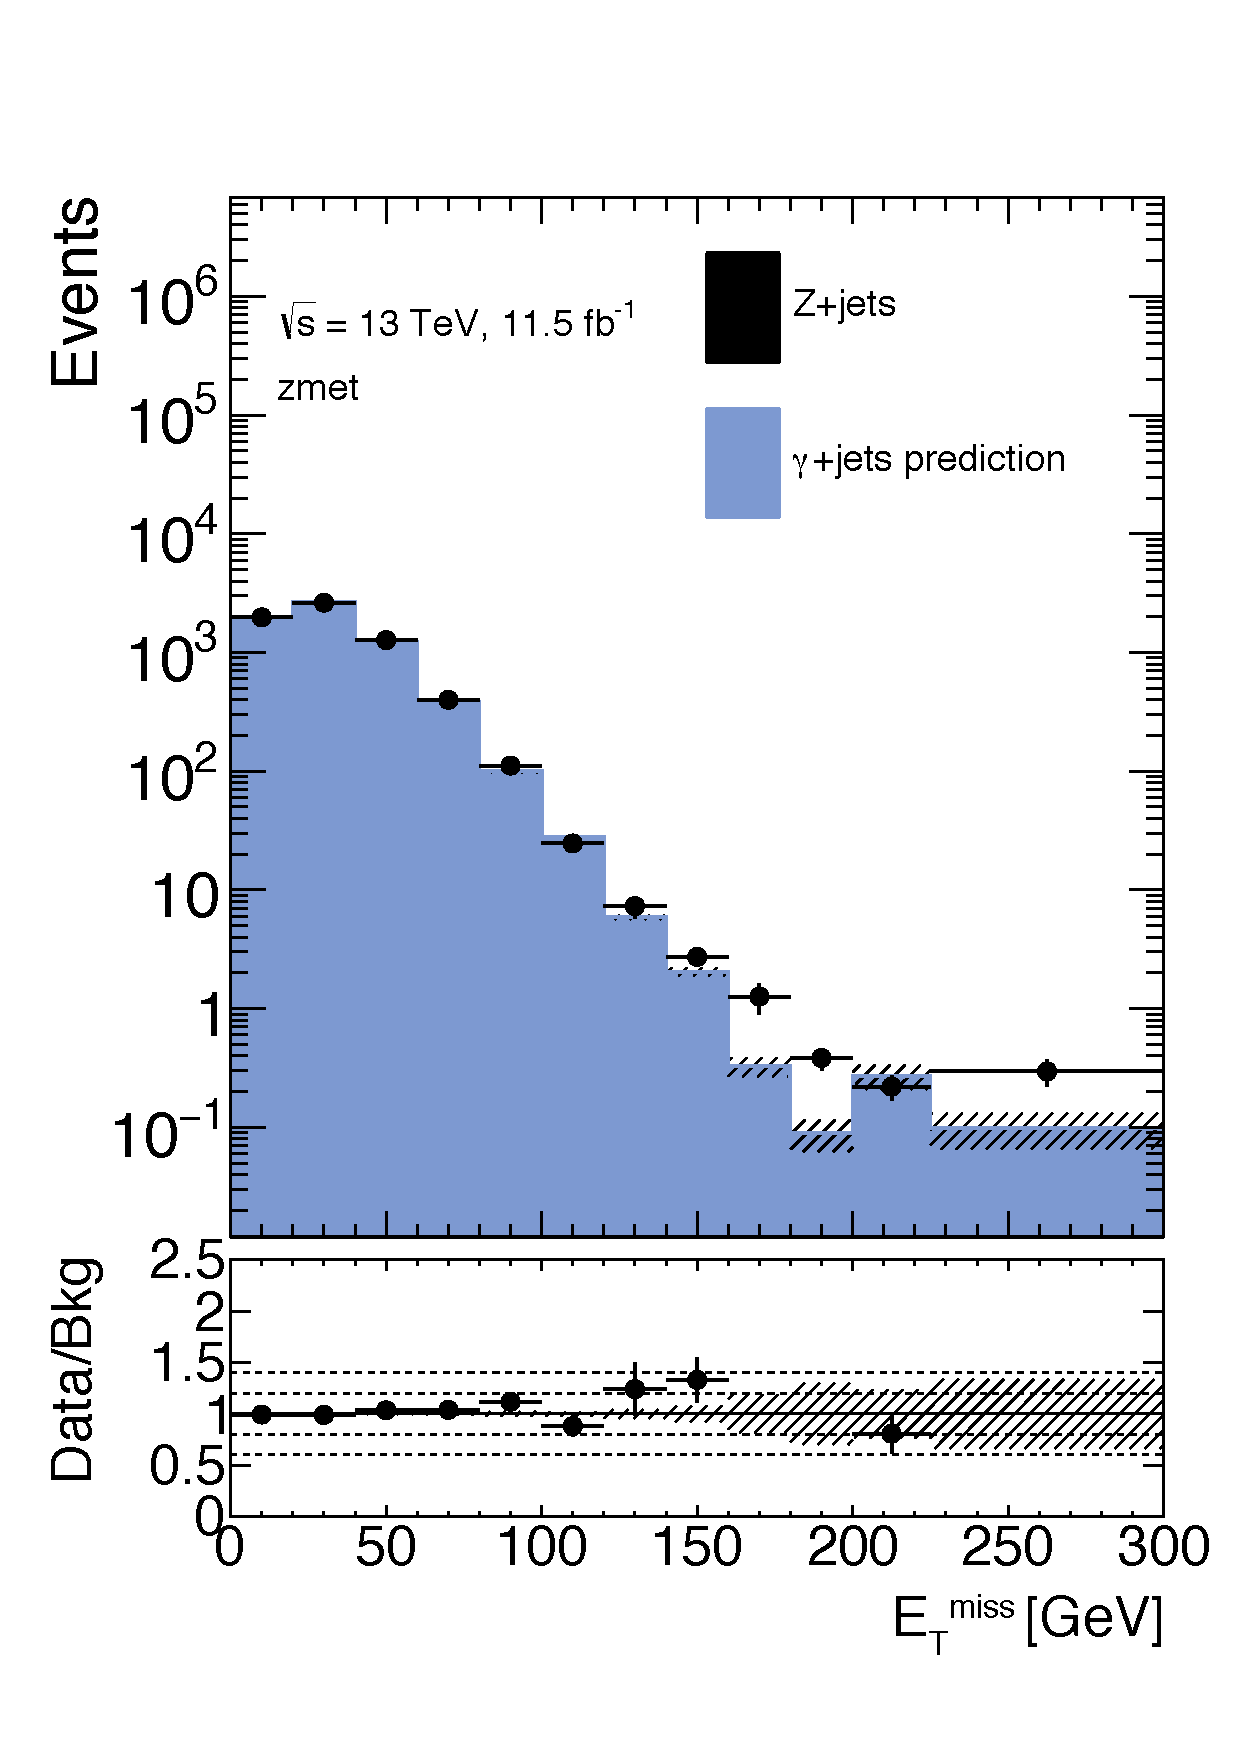
\includegraphics[width=.45\linewidth]{figures/photons/MC_hist_met_plot_ee_2j_2016_mcmetl_ptrw__zmet_.pdf}
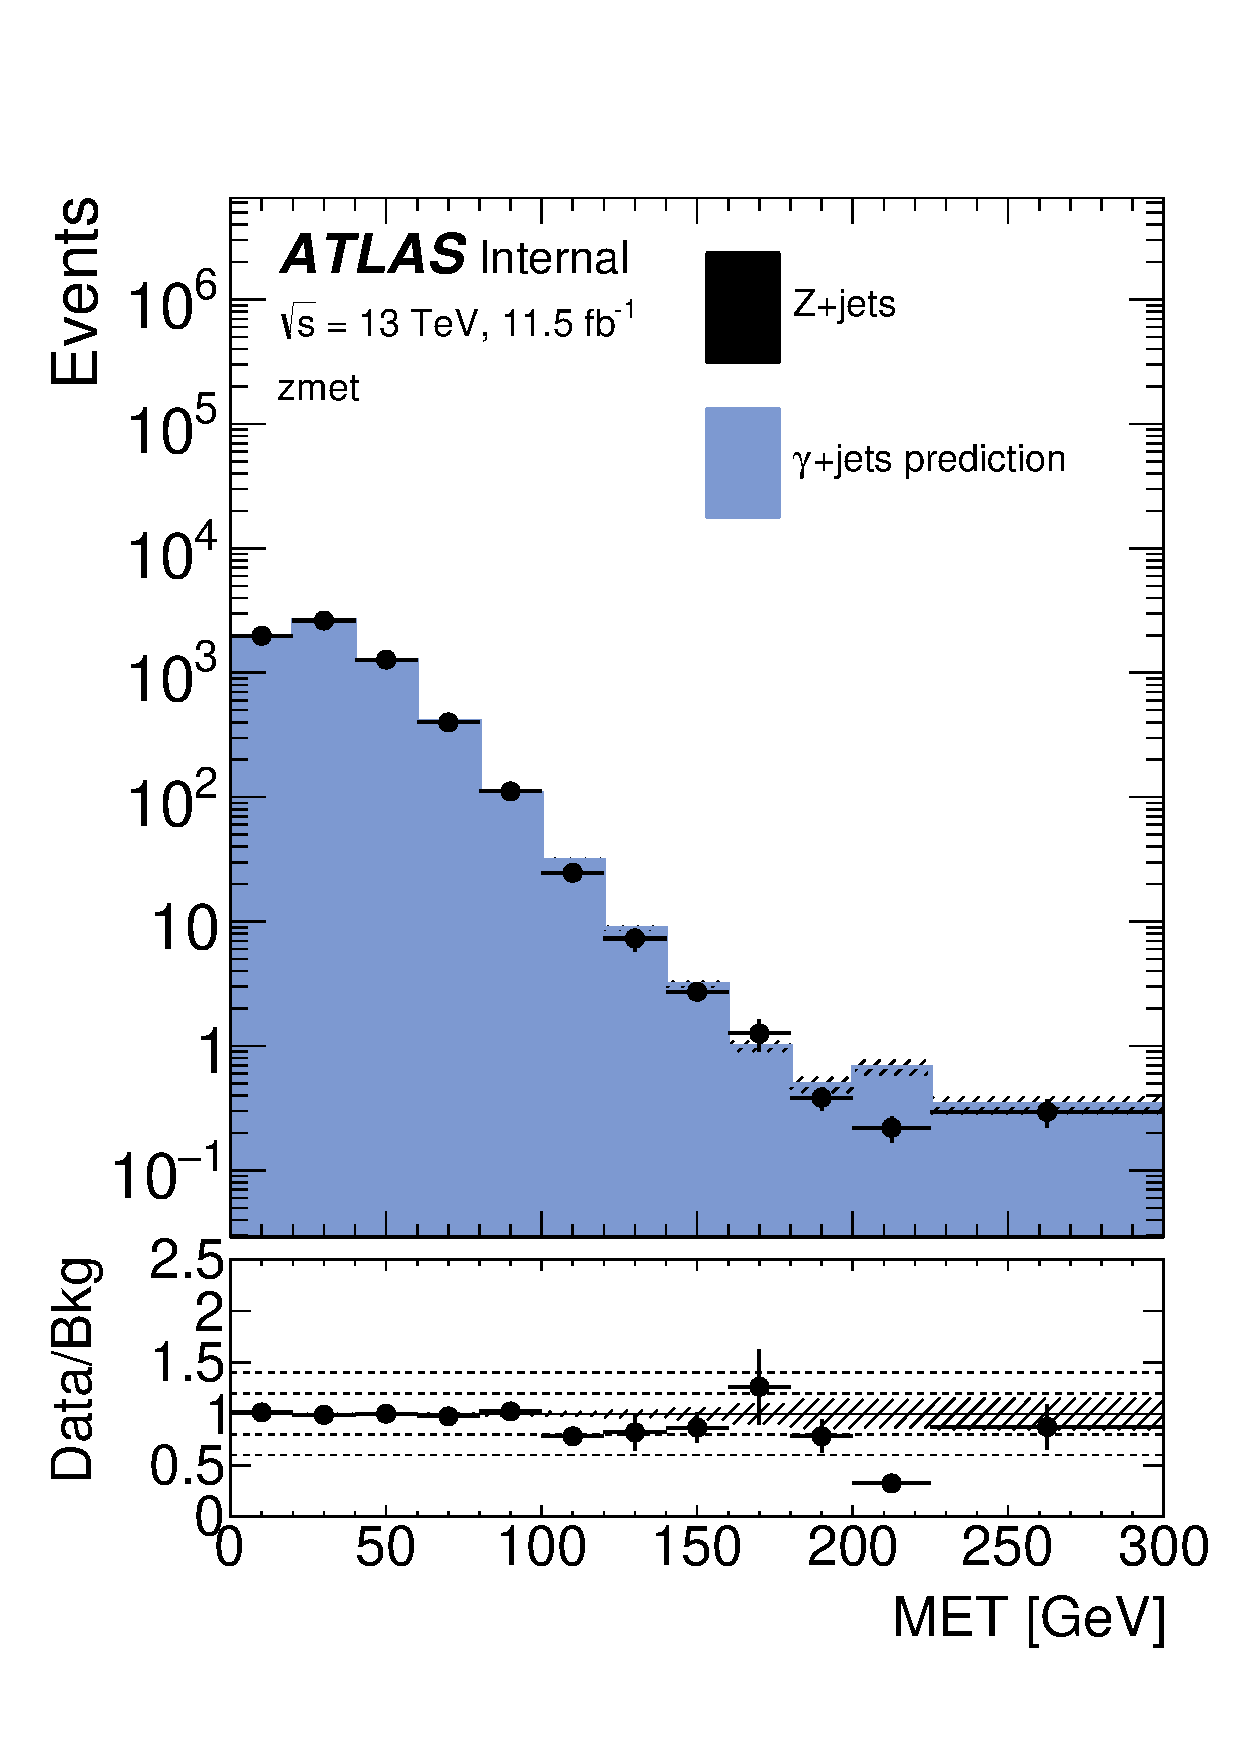
\includegraphics[width=.45\linewidth]{figures/photons/MC_hist_met_plot_ee_2j_2016_mcmetl_ptsmrw_smear_zmet_.pdf}
\caption{\met distribution comparing \ac{MC} distributions of photon and $Z$ events before any smearing is applied (top), with only \pt reweighting applied (bottom left), and after \pt reweighting and smearing have both been applied (bottom right) in the $ee$ channel of 2016 data. }
\label{fig:photon_metchange_ee}
\end{figure}
\end{centering}

\begin{centering}
\begin{figure}[!hbt]
\myfloatalign
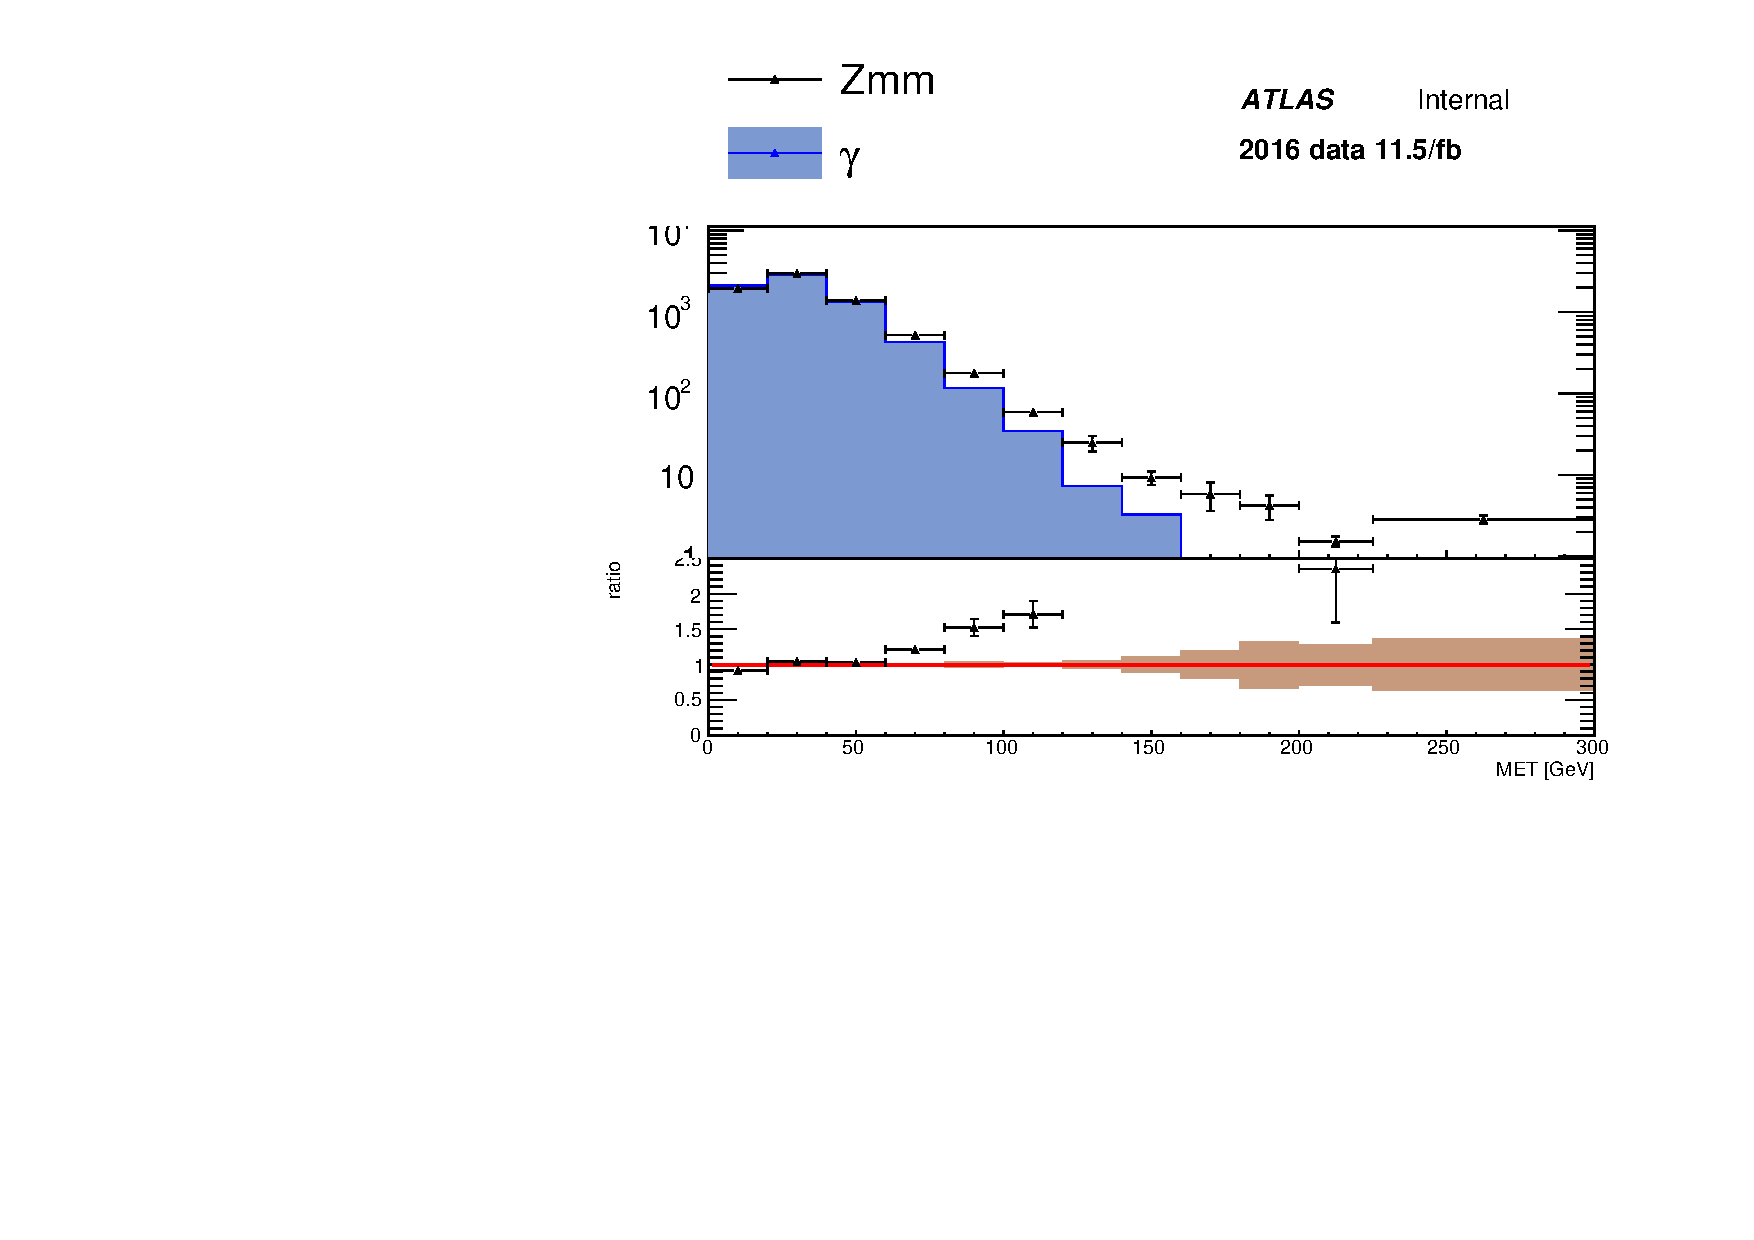
\includegraphics[width=.75\linewidth]{figures/photons/Photon_Zmm_met_2j_2016_mcmetl___zmet.pdf}
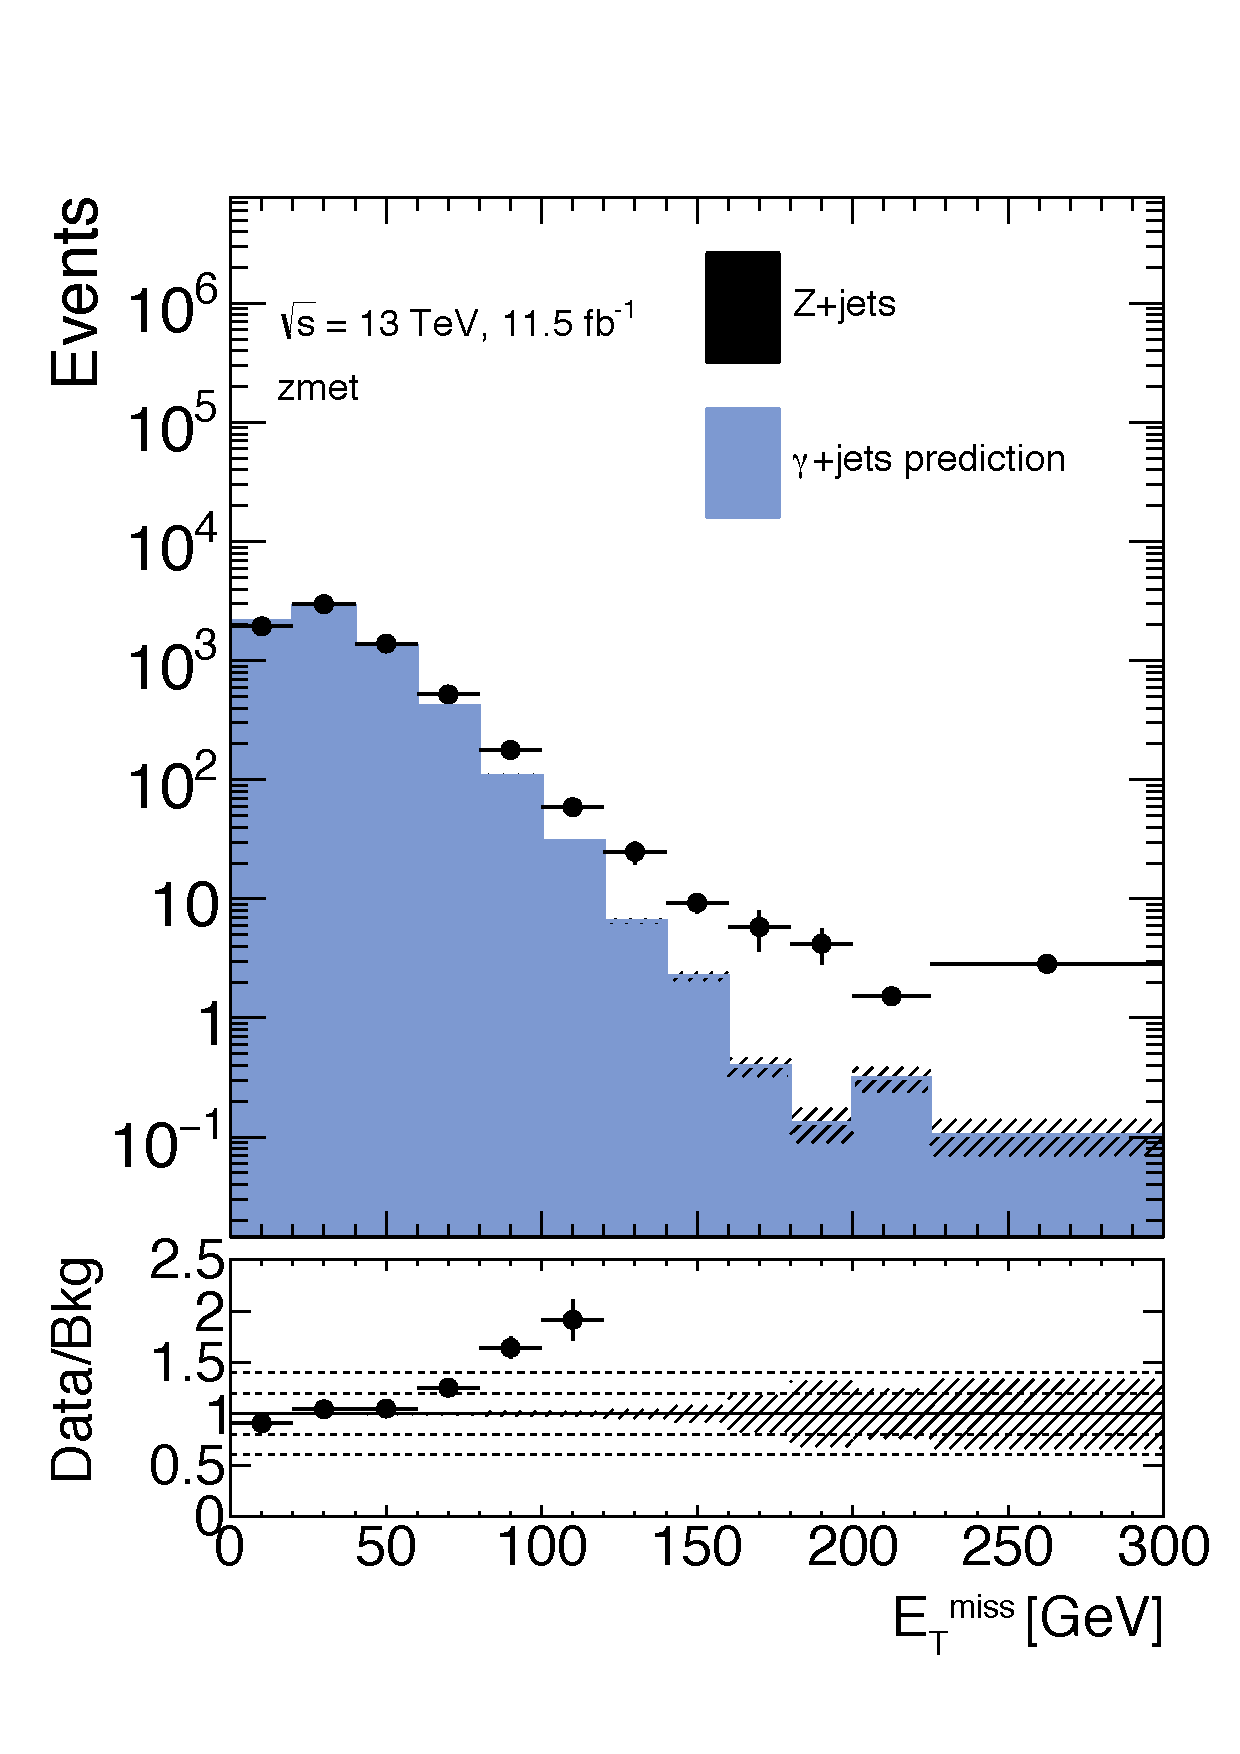
\includegraphics[width=.45\linewidth]{figures/photons/MC_hist_met_plot_mm_2j_2016_mcmetl_ptrw__zmet_.pdf}
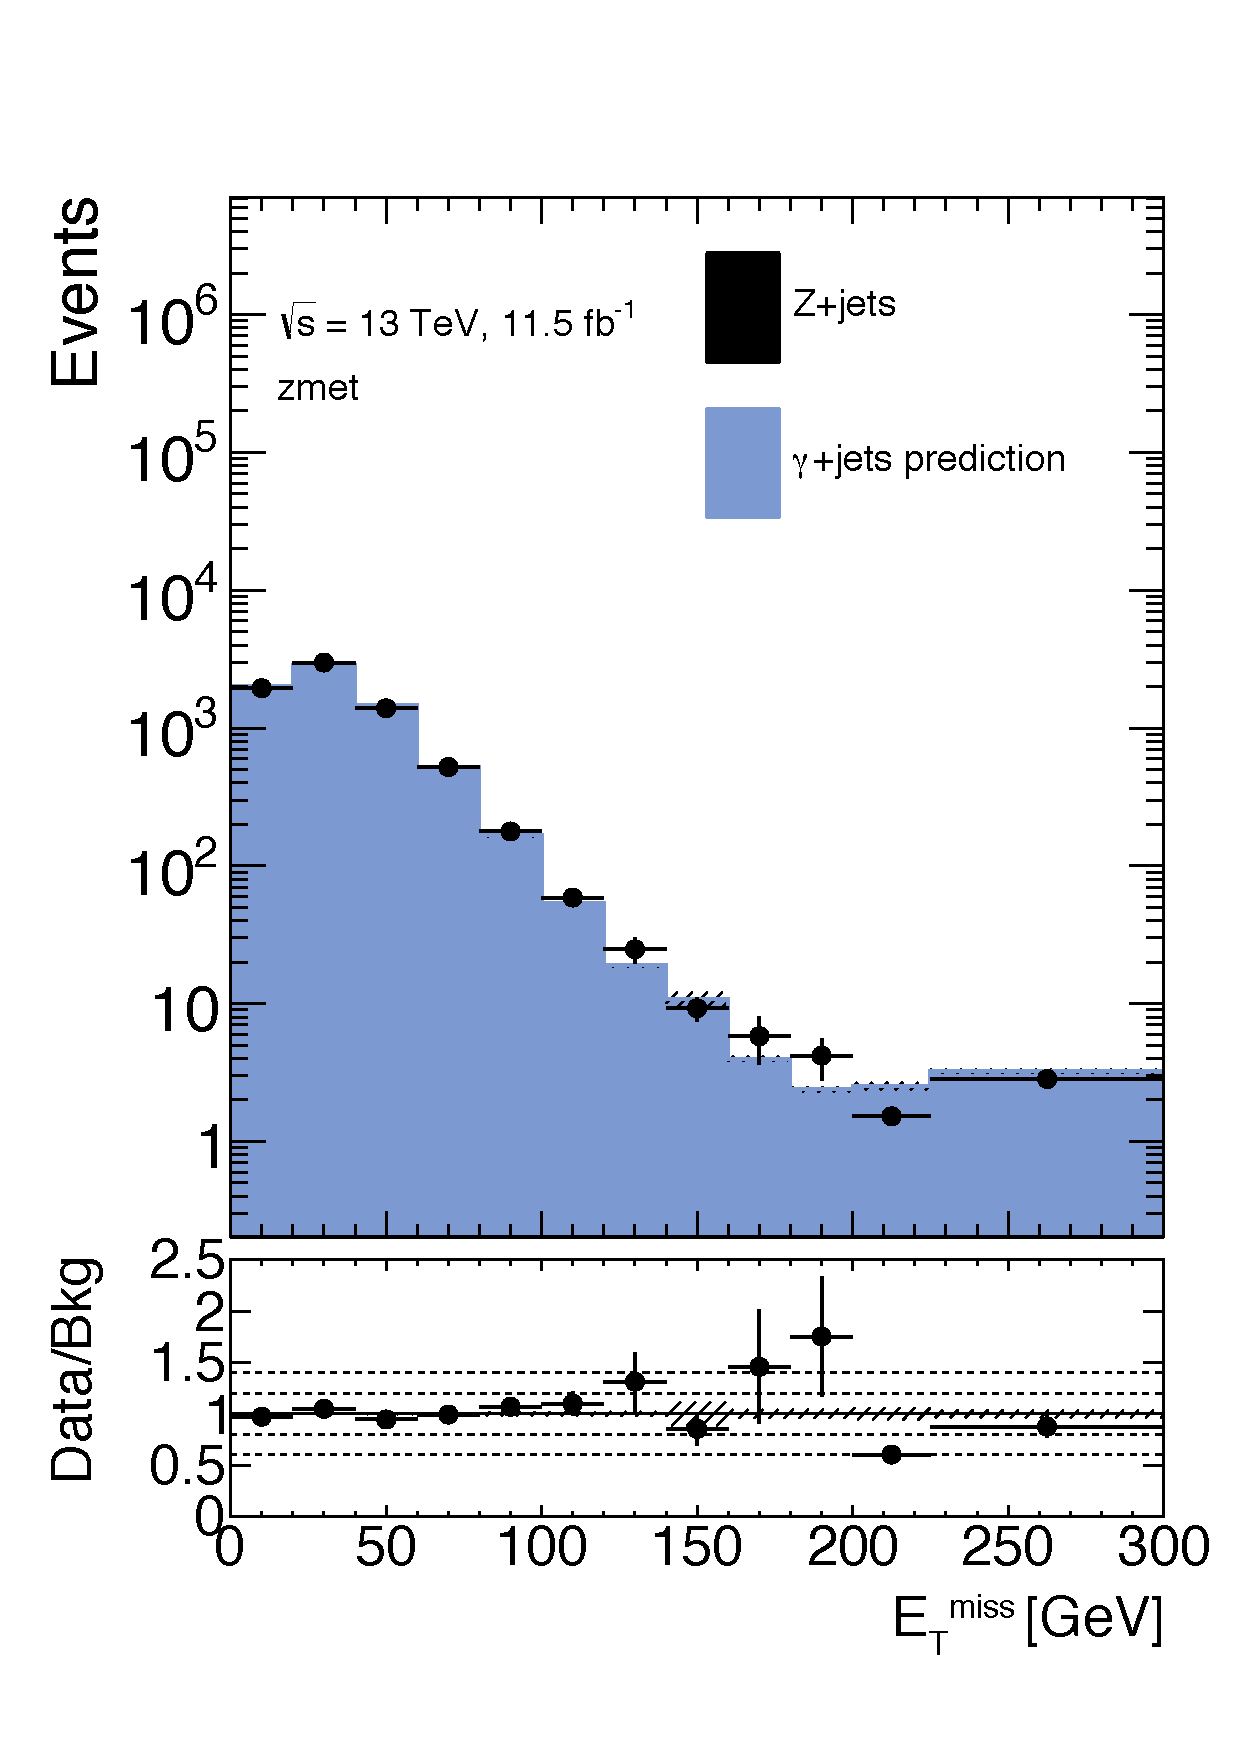
\includegraphics[width=.45\linewidth]{figures/photons/MC_hist_met_plot_mm_2j_2016_mcmetl_ptsmrw_smear_zmet_.pdf}
\caption{\met distribution comparing \ac{MC} distributions of photon and $Z$ events before any smearing is applied (top), with only \pt reweighting applied (bottom left), and after \pt reweighting and smearing have both been applied (bottom right) in the $\mu\mu$ channel of 2016 data.}
\label{fig:photon_metchange_mm}
\end{figure}
\end{centering}

With the \met distribution of the \dyjets events correctly emulated by the modified \gjets events, the $\Delta\phi(\text{jet}_{12},{\boldsymbol p}_{\mathrm{T}}^\mathrm{miss})$ cut can be applied. Then, the \gjets distribution is normalized to match the \dyjets yield in CRZ, a region identical to SRZ, but with a maximum \met value of 60 \gev. This yield is determined by subtracting all other backgrounds from the number of data events observed in CRZ, with each background estimated according to its nominal background prediction for the \ac{SR}. 

\subsection{Determining \HT and \mll}
\label{sec:photon_mll}

One complication thus far ignored is that CR-$\gamma$ has no leptons, but some quantities that define the \ac{SR} require them, namely \mll~and \HT. There is no analogue of \mll~in photon events, and though the contribution of leptons to the \HT variable can be related to the \pt of the boson in \gjets events, the relationship depends on the angular distributions between lepton pairs in \dyjets events and must account for the mass of the $Z$ boson. Instead of determining an analytic function to describe such a relation, both of these variables are determined by creating histograms binned in the boson \pt and sampling. 

In the case of \HT, distributions of the scalar sum of the \pt of the leading leptons are made for each $Z$ boson \pt bin using \dyjets \ac{MC}. A sampled value from the distribution is then added to the \HT of the jets in a photon event to produce the final estimate. This sampling is done before any reweighting is performed because the \HT is needed to make the preselection for the reweighting process. However, the smearing is performed inclusively in \HT, so this procedure can be performed using the smeared photon \pt to choose the distribution to sample. 

The \mll~determination is performed after both the smearing and reweighting, and is tied closely to the smearing step. Mismeasurements in lepton \pt can create \met in a \dyjets event, but the same event is likely to migrate off the $Z$ \mll~window due to the mismeasured lepton. Thus it is very important that the two effects be carefully correlated in the manipulated photon events. To achieve this, \ac{MC} $Z$ events from the 1-jet \ac{CR} described in \autoref{sec:photon_smearing} are used to make two-dimensional distributions of \mll~as a function of the difference between reconstructed and true $Z$ \pt for the $ee$ and $\mu\mu$ channels. A photon event then uses the $\Delta$\pt assigned to it during the smearing process to index the distribution, and an \mll~value is sampled from the corresponding bin \footnote{Ideally this $\Delta$\pt would also include the difference between the true and reconstructed \pt of the photon events, but this information is of course not accessible in data. Luckily, in the events in the final \ac{SR} this value is typically negligible compared to the $\Delta$\pt from smearing, so the impact is small.}. 

To test the soundness of this procedure, it is repeated purely in \ac{MC}, and the results of the \ac{MC} prediction and the data prediction are compared to the \mll~distribution in \dyjets \ac{MC} in \autoref{fig:photon_mll_mc}. Though there are some areas of disagreement across the \mll~spectrum, very good closure is seen on the on-$Z$ bin, which is what is needed for the estimate of SRZ's backgrounds. After the \mll~distribution has been emulated, a cut requiring that the photon events have an \mll~value between 81 and 101 \gev~can be made.

\begin{centering}
\begin{figure}[!hbt]
\myfloatalign
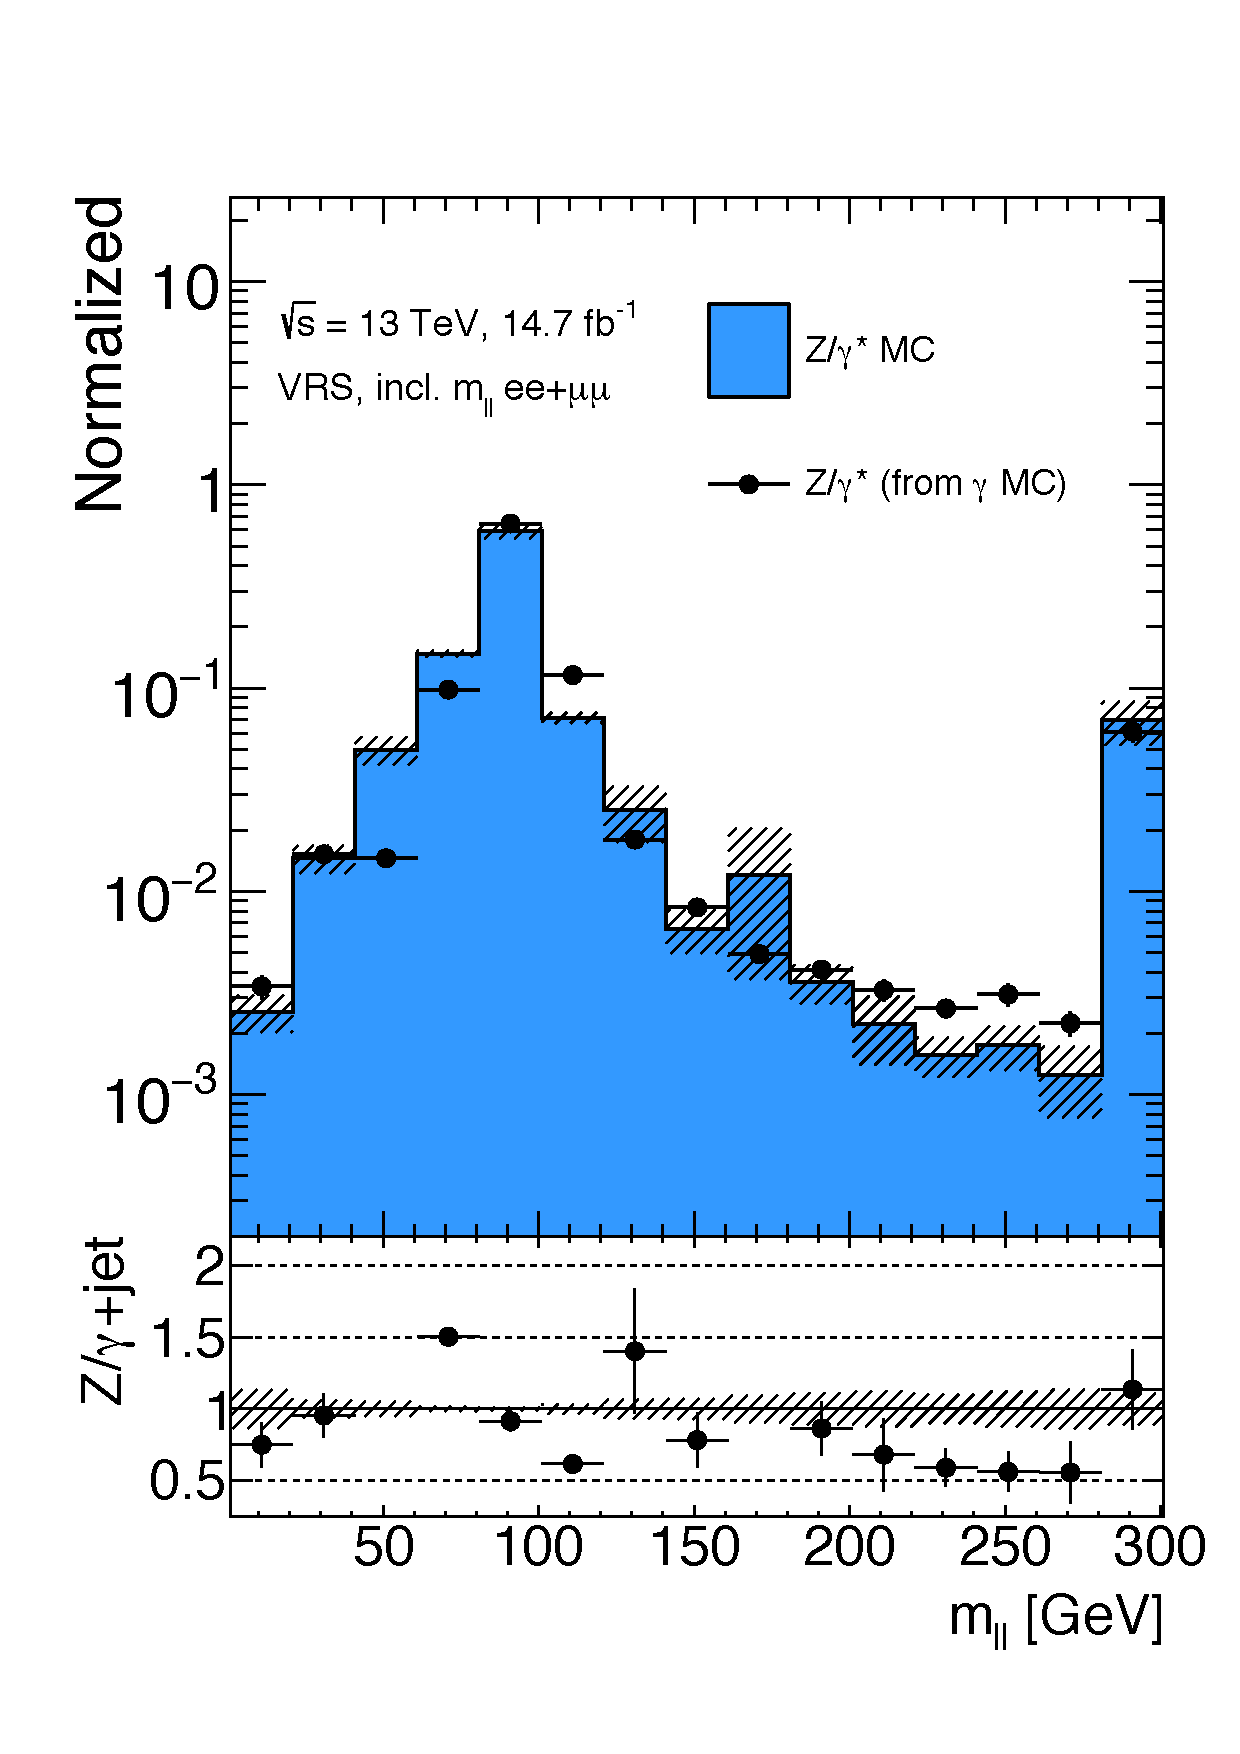
\includegraphics[width=.45\linewidth]{figures/photons/DataMC_GJ_ee+mm_zmet_GMC.pdf}
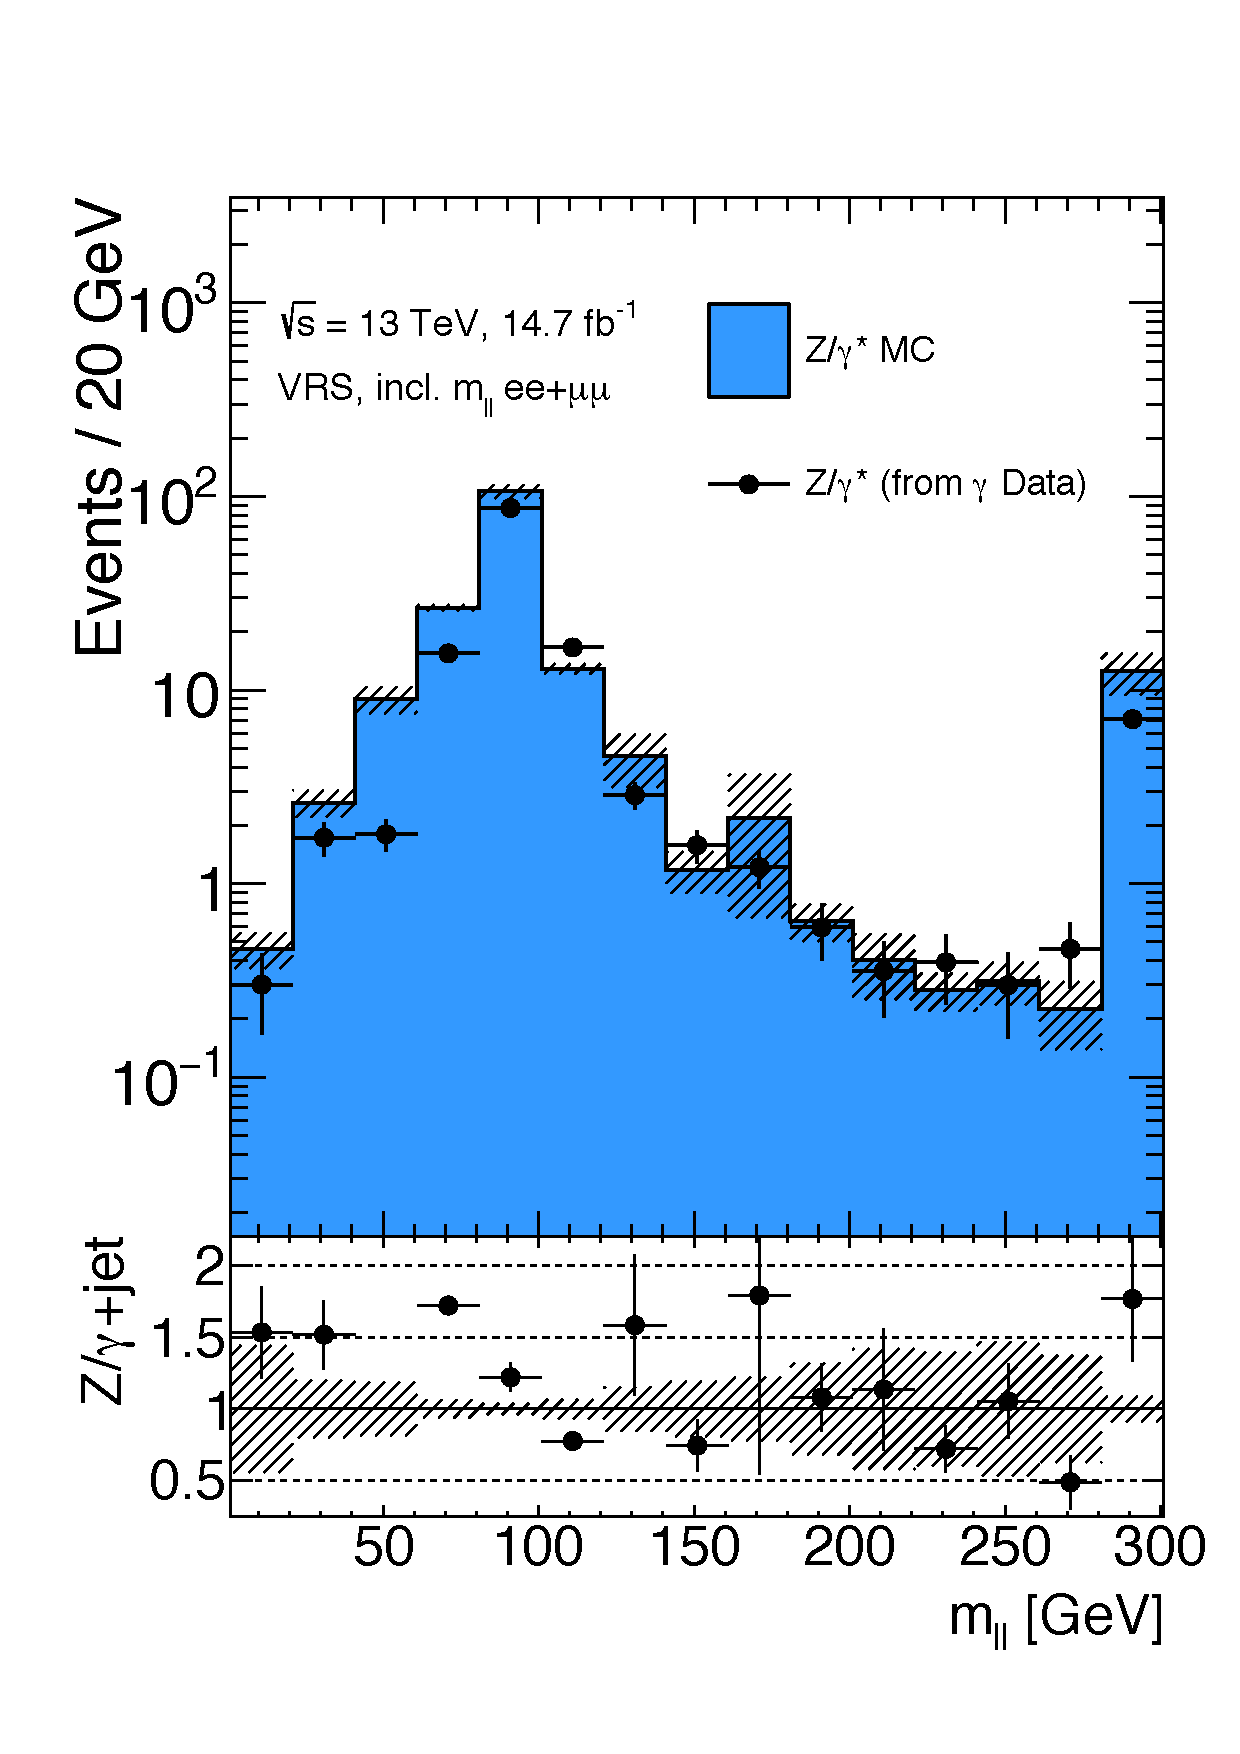
\includegraphics[width=.45\linewidth]{figures/photons/DataMC_GJ_ee+mm_zmet_ZMC.pdf}
\caption{\dyjets \ac{MC} \mll~distribution compared to the prediction from \gjets method performed on \ac{MC} (left) and the prediction from \gjets method performed on data (right).}
\label{fig:photon_mll_mc}
\end{figure}
\end{centering}

\subsection{Subtraction of $V\gamma$ Events}
\label{sec:gjets_vg}

At high \met, where the signal region lies, contamination of CR-$\gamma$ with $V\gamma$ events becomes significant, as shown in \autoref{fig:photon_vgamma}. These events must be subtracted from the \gjets prediction because, once the photons are corrected to approximate $Z$s, they essentially provide a (not very accurate) prediction of diboson events, which are already accounted for in another background estimate. 

\begin{centering}
\begin{figure}[!hbt]
\myfloatalign
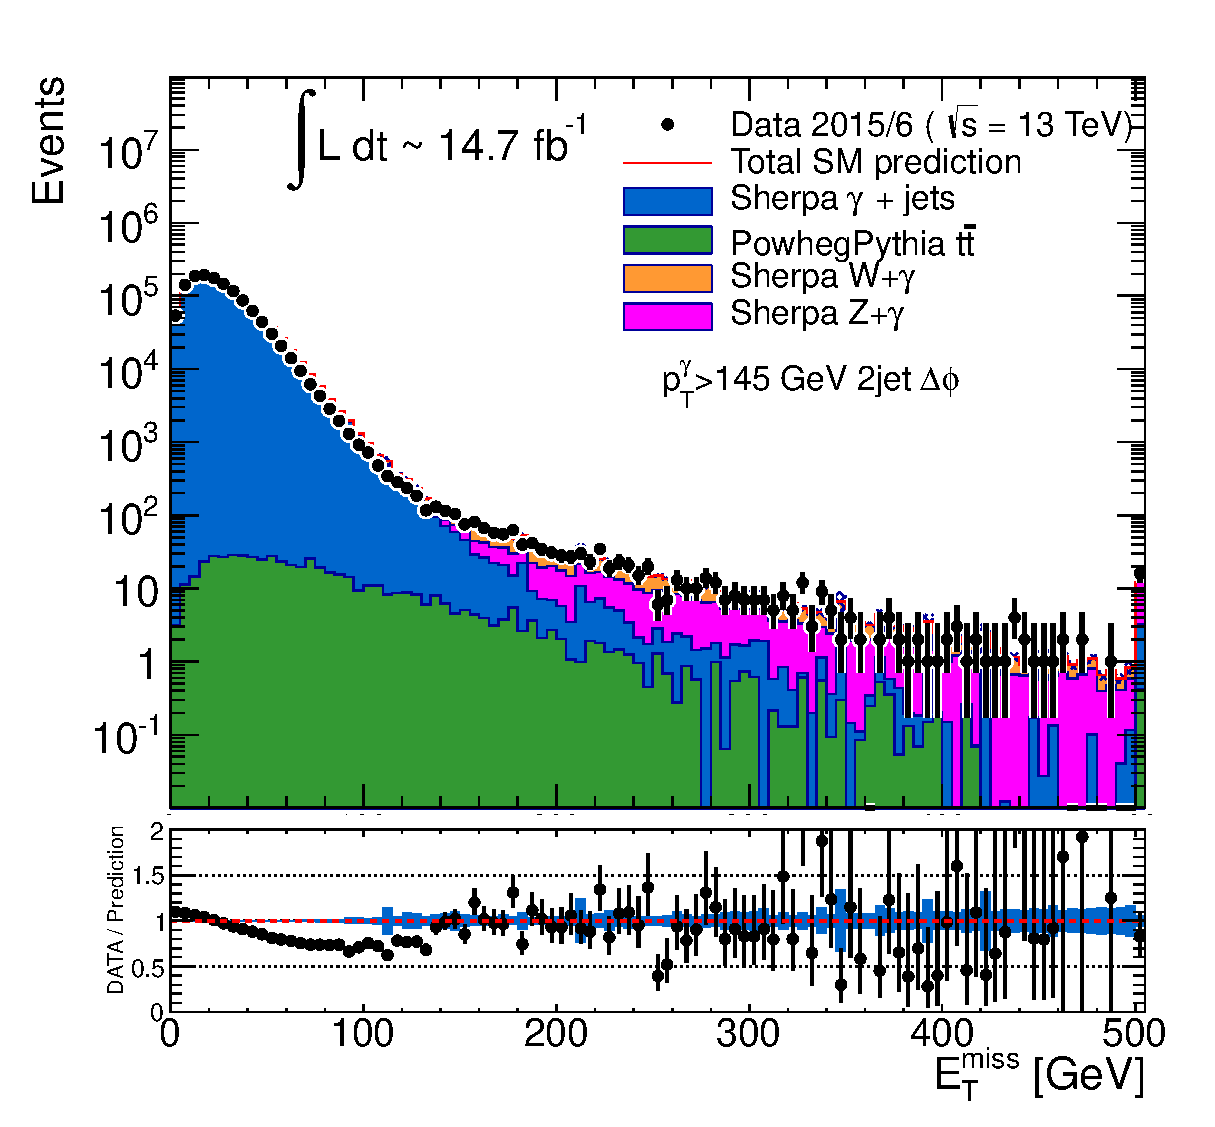
\includegraphics[width=.90\linewidth]{figures/photons/hPhot_Met_dPhiJet_hist.eps}
\caption{Comparison of data and \ac{MC} in CR-$\gamma$ without any \HT cut, including the contributions from various $V\gamma$ processes.}
\label{fig:photon_vgamma}
\end{figure}
\end{centering}

This subtraction is accomplished by applying the \gjets method to $V\gamma$ \ac{MC} to approximate these backgrounds' contribution to the final \met distribution. This contribution is then subtracted from the \gjets prediction, the impact of which can be seen in \autoref{fig:photon_vgamma_subt}. As expected, the impact is greatest at high \met where these backgrounds are most significant.

\begin{centering}
\begin{figure}[!hbt]
\myfloatalign
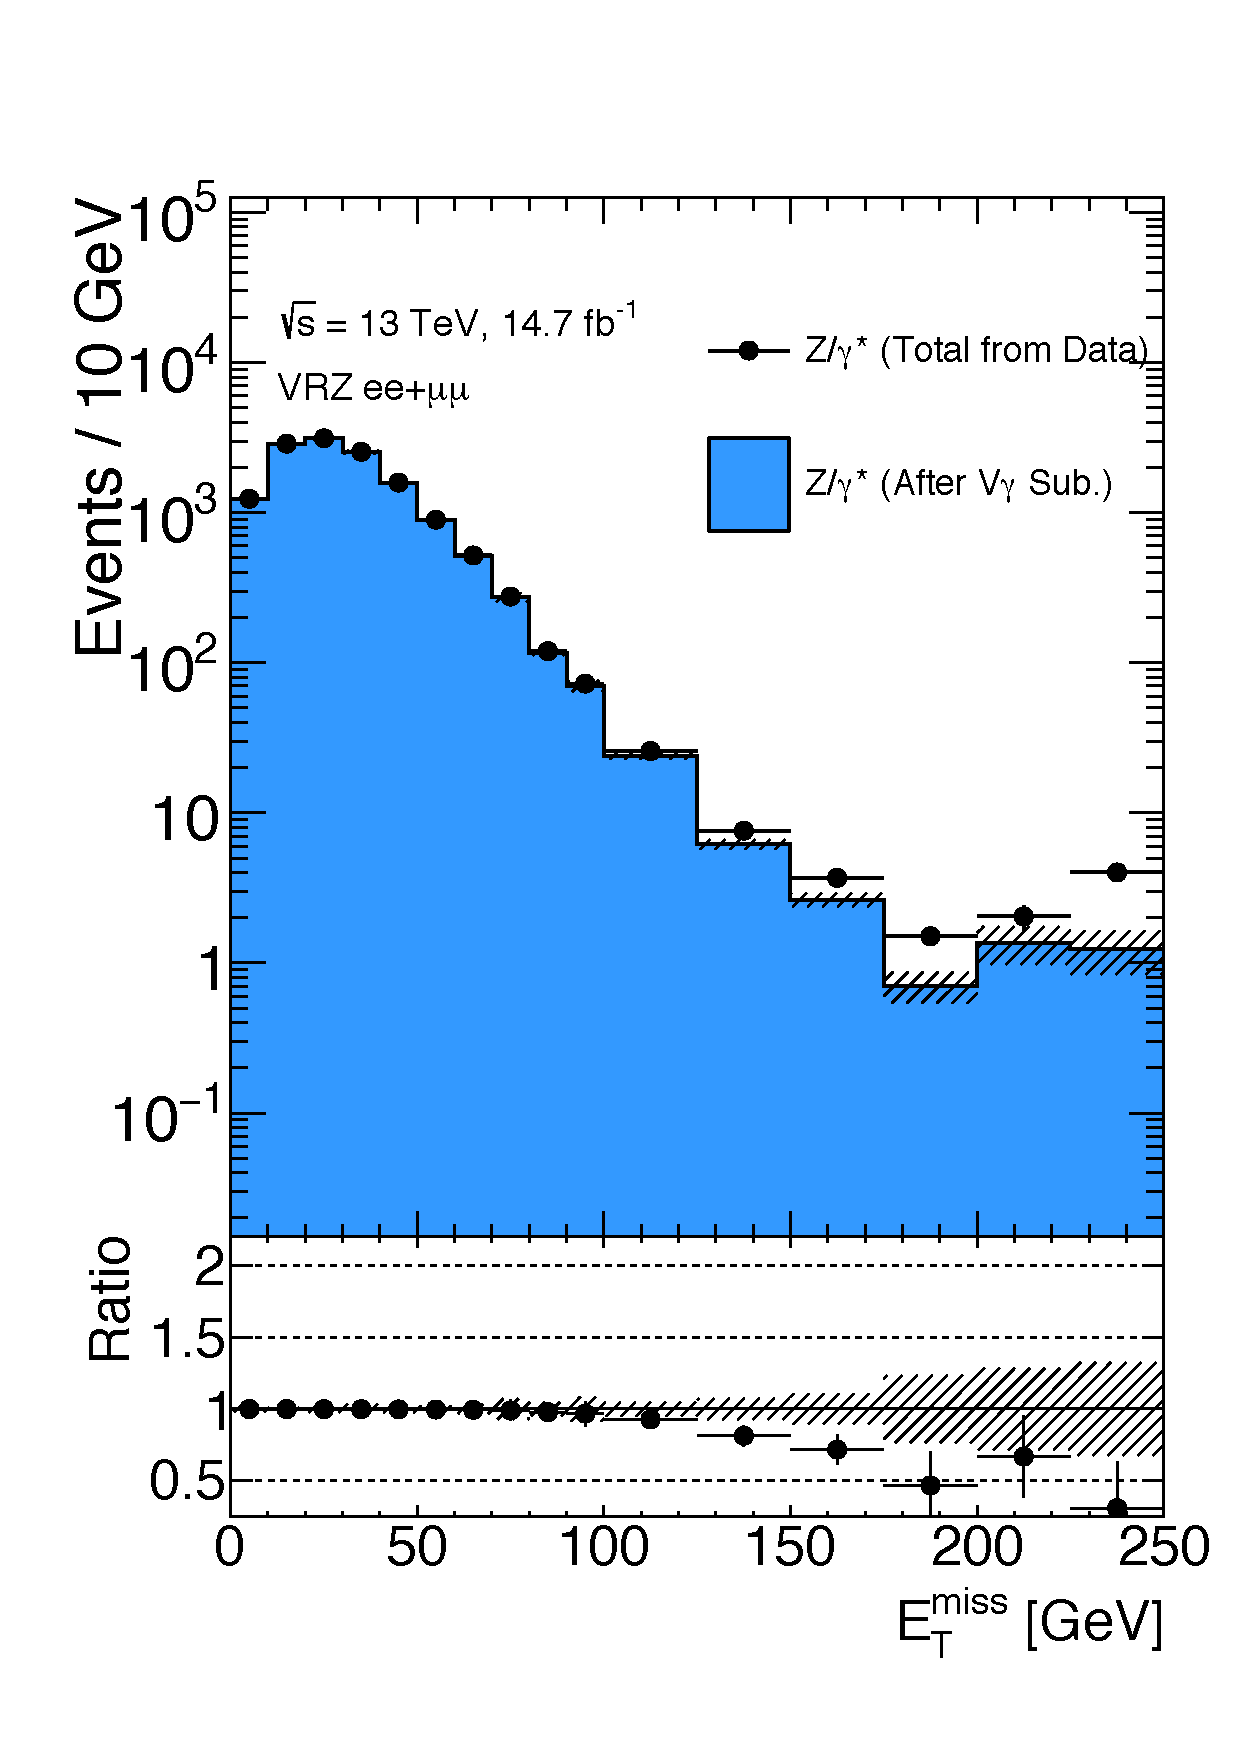
\includegraphics[width=.90\linewidth]{figures/photons/Vgamma_MET_ee+mm_zmet_onz.pdf}
\caption{Total \gjets data prediction in SRZ (excluding the \met cut) and the prediction after the $V\gamma$ subtraction.}
\label{fig:photon_vgamma_subt}
\end{figure}
\end{centering}

\subsection{Validation in Data}

The \gjets jets method is validated in a region called VRZ, defined in \autoref{tab:regions-z}, which is similar to SRZ, but with an inverted \met cut. \autoref{fig:photon_validation} shows the low-\met portion of this \ac{VR} where the \dyjets background is dominant. Here, the three data-driven background estimates, as well as the remaining \ac{MC} backgrounds are stacked and compared to the data yield in this region, demonstrating excellent agreement across a wide \met range. 

\begin{centering}
\begin{figure}[!hbt]
\myfloatalign
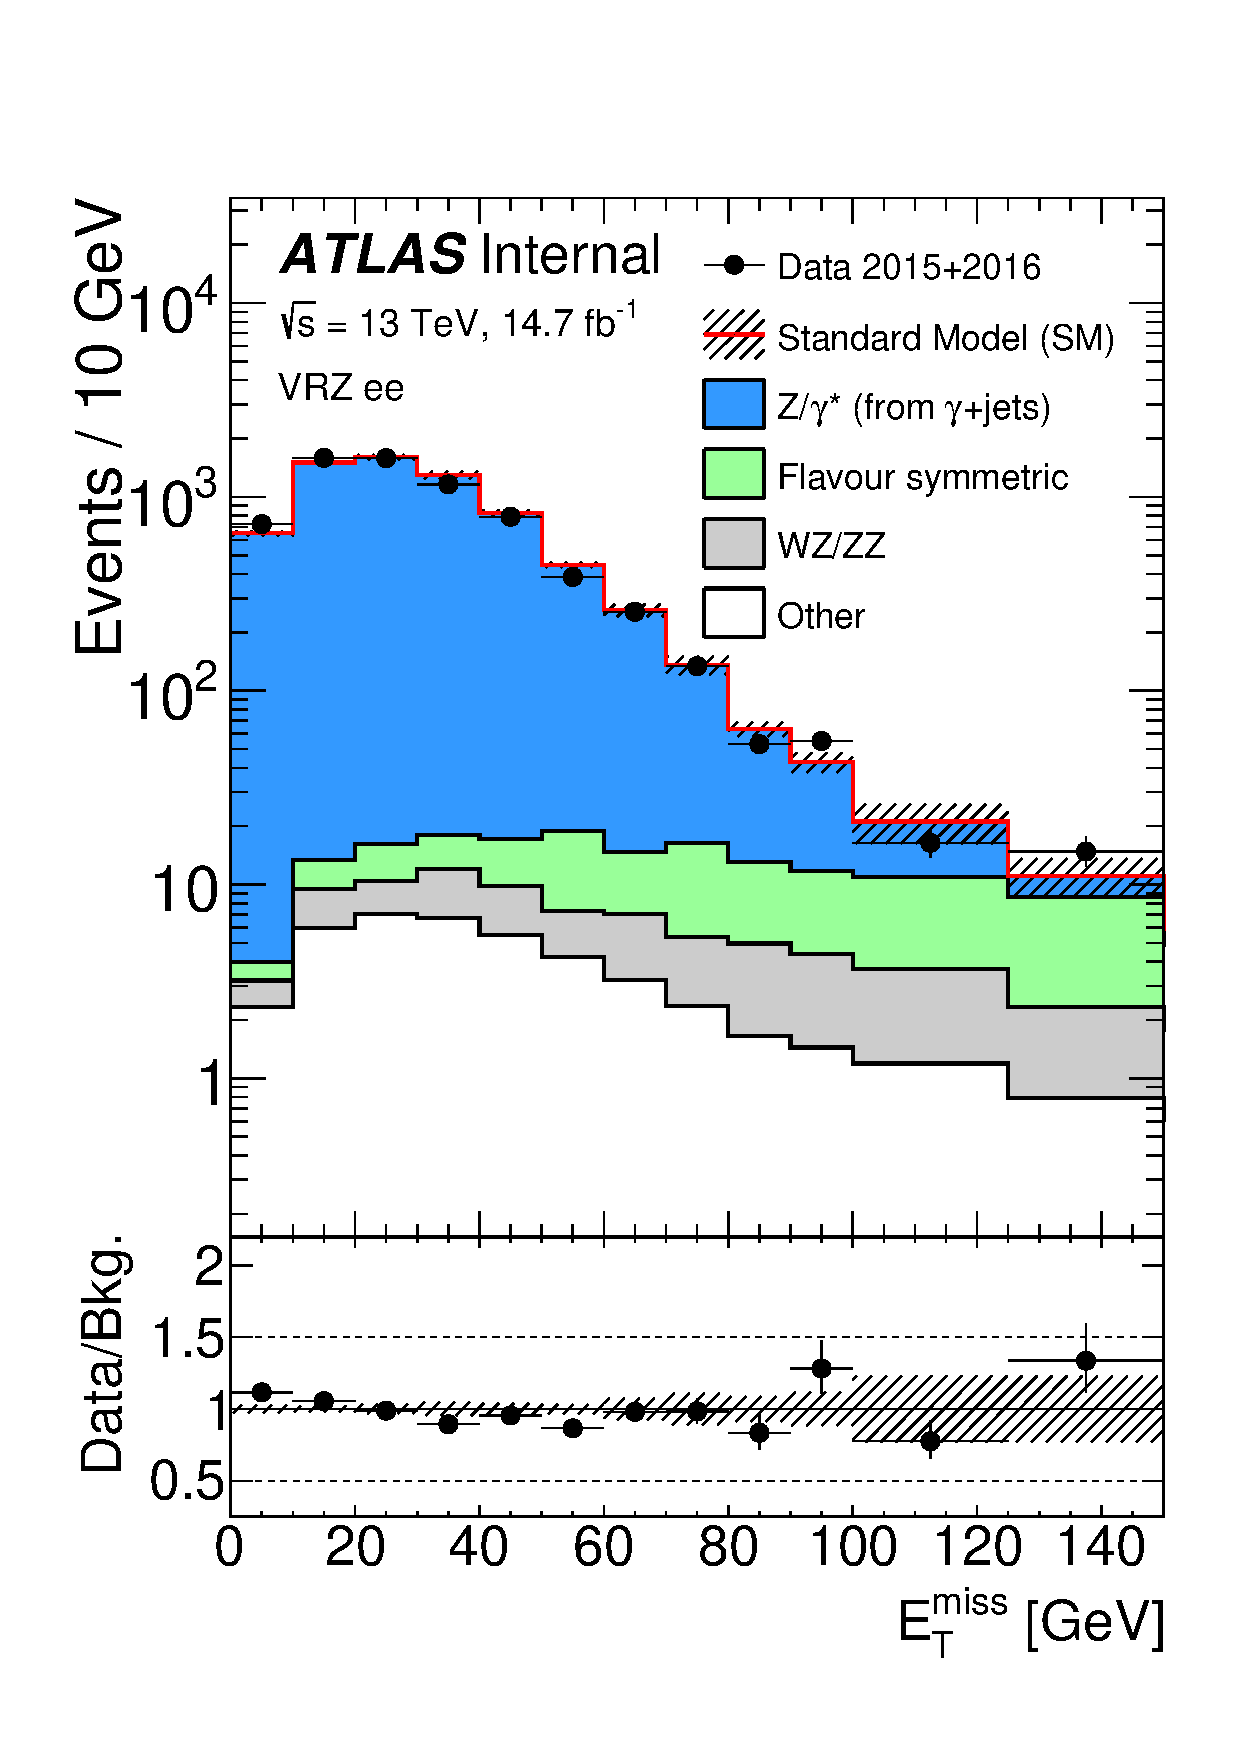
\includegraphics[width=.45\linewidth]{figures/photons/MET_azmet_ee_onz.pdf}
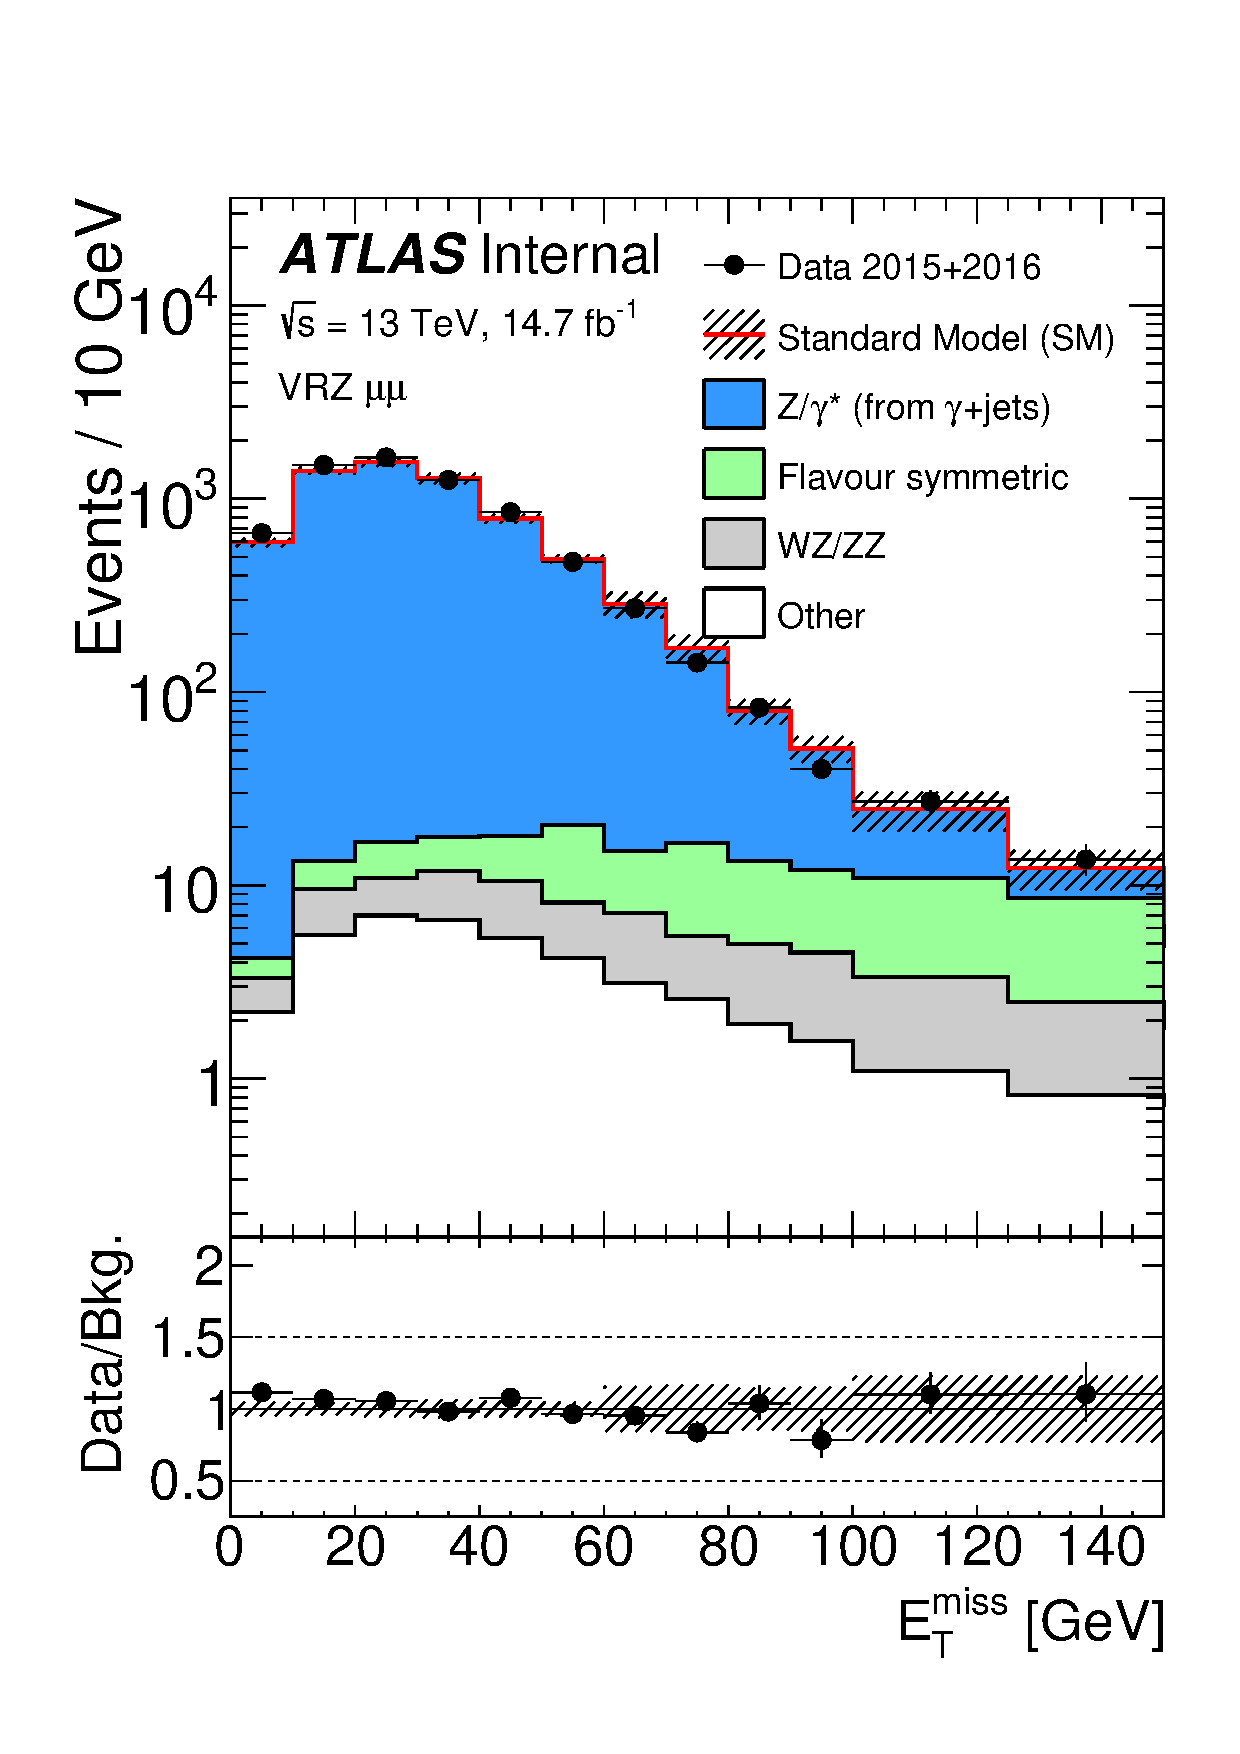
\includegraphics[width=.45\linewidth]{figures/photons/MET_azmet_mm_onz.pdf}
\caption{\MET distribution in VRZ $ee$ (left) and $\mu\mu$ (right) with total data yield compared to the sum of the prediction from the \gjets method, the prediction from the flavor symmetry method, the prediction from the fake background estimation (included under ``other''), and the remaining backgrounds taken from \ac{MC}.}
\label{fig:photon_validation}
\end{figure}
\end{centering}

An additional check can be made in VRZ by removing the $\Delta\phi(\text{jet}_{12},{\boldsymbol p}_{\mathrm{T}}^\mathrm{miss})$ intended to supress the \dyjets background from jet mismeasurement. \autoref{fig:photon_dphi} shows the distribution of this variable in VRZ, and demonstrates that, even at low values where the \dyjets background is dominant, the \gjets method models it accurately.

\begin{centering}
\begin{figure}[!hbt]
\myfloatalign
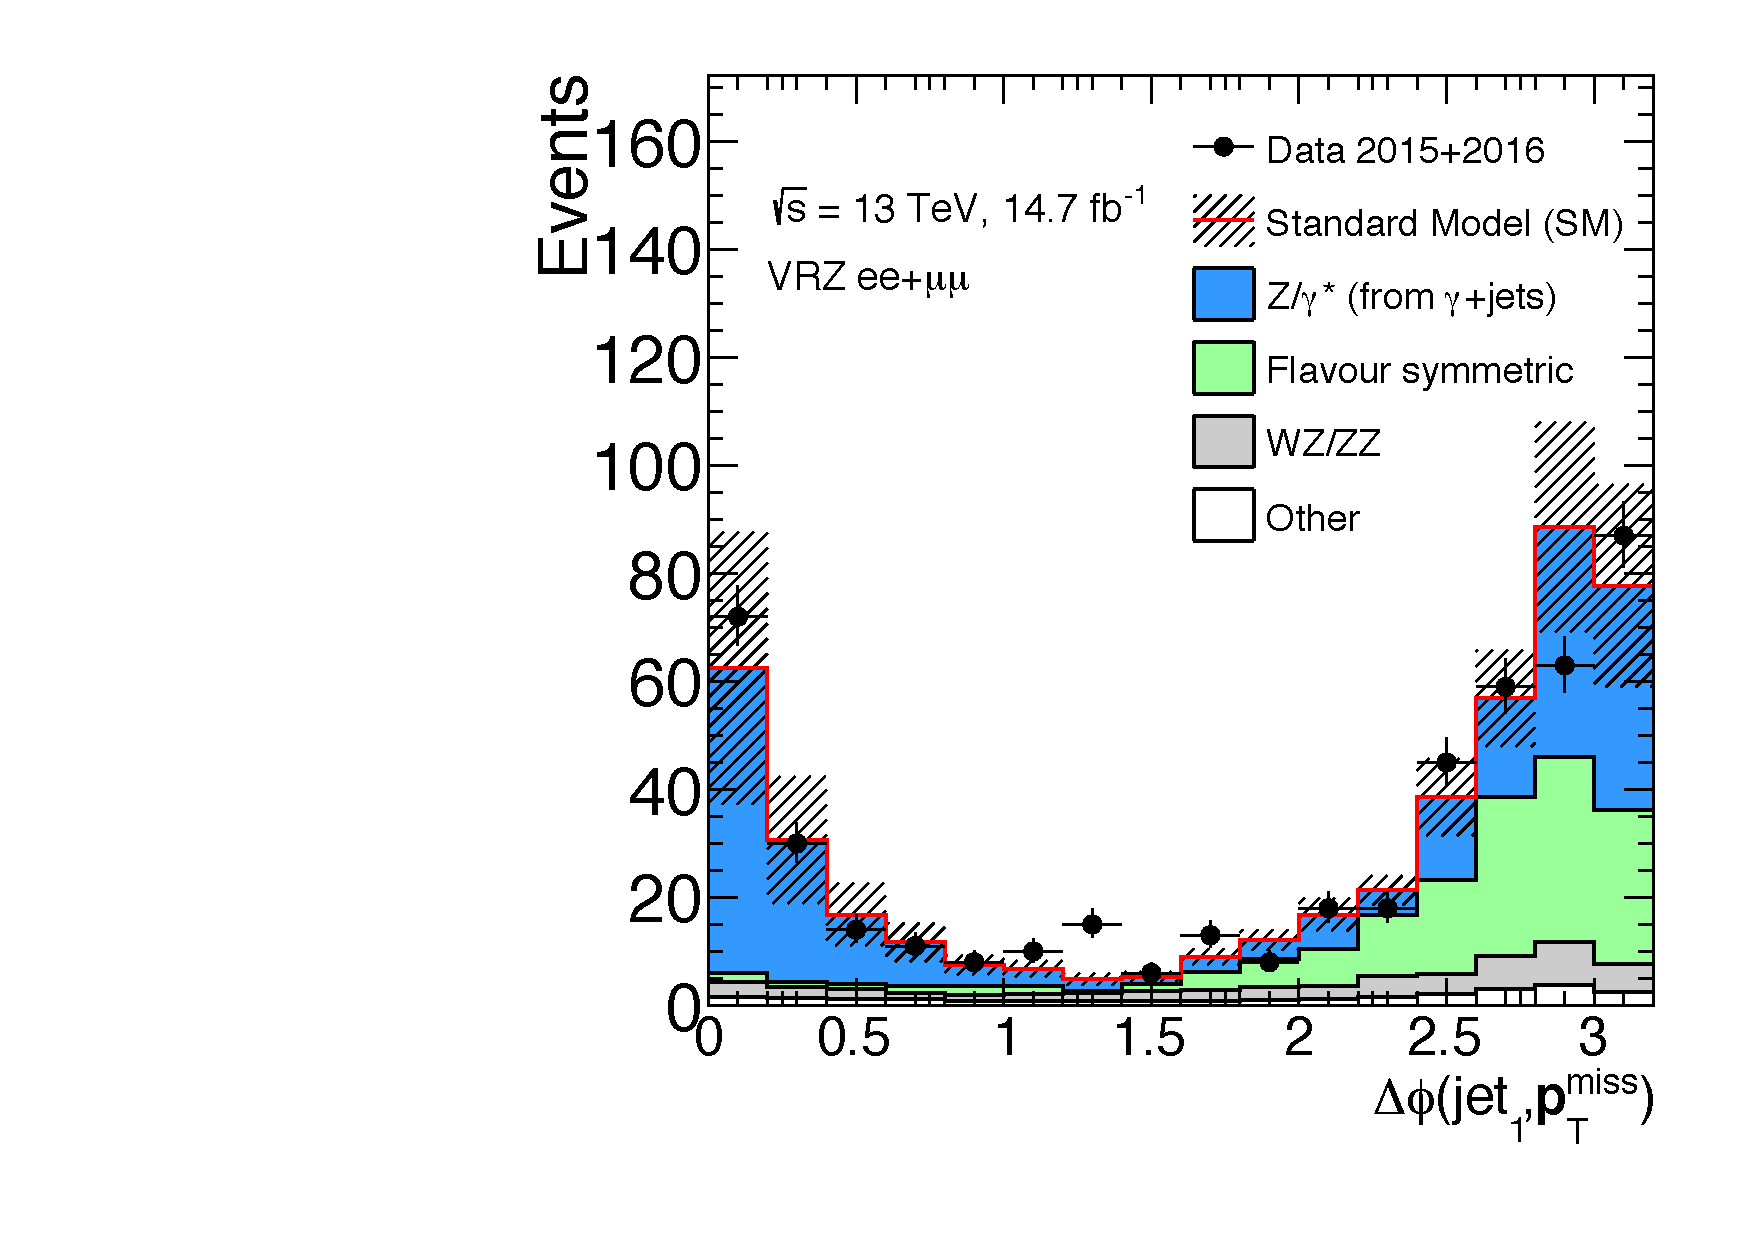
\includegraphics[width=.45\linewidth]{figures/photons/METJetLeading_azmet_ee+mm_onz_VR.pdf}
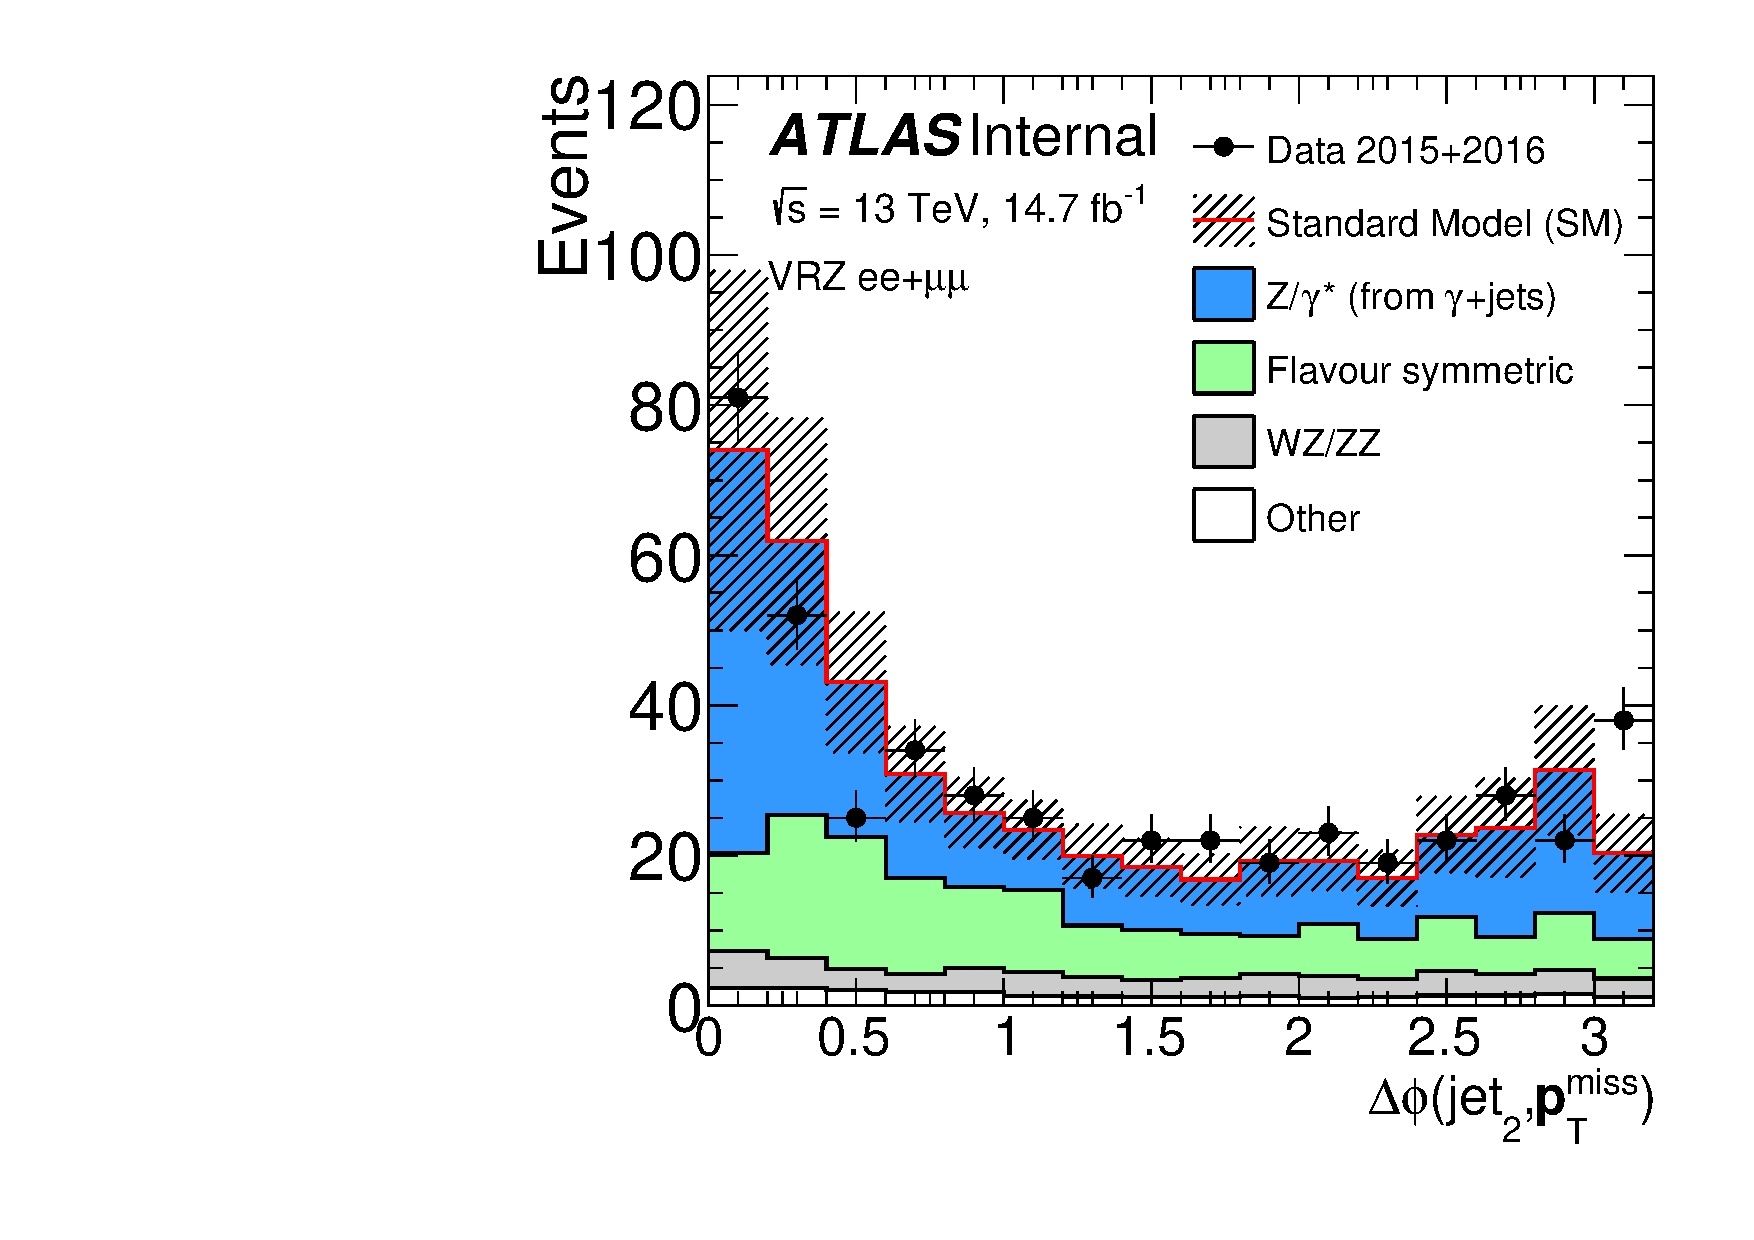
\includegraphics[width=.45\linewidth]{figures/photons/METJetSecond_azmet_ee+mm_onz_VR.pdf}
\caption{ $\Delta\phi(\text{jet},{\boldsymbol p}_{\mathrm{T}}^\mathrm{miss})$ distribution in for the leading jet (left) and the subleading jet (right). The comparison is performed in VRZ with the cut on $\Delta\phi(\text{jet}_{12},{\boldsymbol p}_{\mathrm{T}}^\mathrm{miss})$ removed.  The total data yield is compared to the sum of the prediction from the \gjets method, the prediction from the flavor symmetry method, the prediction from the fake background estimation (included under ``other''), and the remaining backgrounds taken from \ac{MC}.}
\label{fig:photon_dphi}
\end{figure}
\end{centering}

%-------------------------------------------------------------------------------------

\section{Fake and Non-Prompt Leptons}
\label{sec:bg-fake}

The \textit{fakes} background consists of processes that produce only one lepton, but whose events are otherwise kinematically similar to those of the \ac{SR}. These processes include semileptonic \ttbar (in which only one of the two $W$ decays results in a lepton), $W$+jets, and single top processes. Though these processes typically only produce one lepton, they can be reconstructed with two leptons due to a hadron being misidentified as a lepton or due to a real non-prompt lepton resulting from photon conversions or $B$-hadron decays. As with the \dyjets background, it is very difficult to predict with \ac{MC} because the failures in reconstruction are typically less well described by the models used in \ac{MC} production than the successes. Nonetheless, a rough estimate can be made of this background by using \ac{MC}, which indicates that the number of fake events in SRZ is consistent with zero. 

To get a more reliable prediction of this background, a data-driven method called the \textit{matrix method} is employed to estimate these fake events \cite{SUSY-2013-20}. This method is also used to estimate the fakes contribution to other control and validation regions where their impact is more significant. 

In the matrix method, the quality requirements for signal leptons are loosened to give a selection of baseline leptons (see \autoref{tab:eledef} and \autoref{tab:muondef}), which consist of a higher fraction of fake leptons. In each \ac{CR}, \ac{VR}, or \ac{SR}, the remaining kinematic selections are made on the baseline leptons, and the number of leptons in the region which pass the signal lepton requirements ($N_{pass}$) and the number which fail ($N_{fail}$) are measured. For a 1-lepton selection, these quantities can be used to predict the number of fake events that pass the selection according to:
%
\begin{equation}
N_{\text{pass}}^{\text{fake}} = \frac{N_{\text{fail}} - (1/\epsilon^{\text{real}} - 1) \times N_{\text{pass}} }{1/\epsilon^{\text{fake}} - 1/\epsilon^{\text{real}}}.
\end{equation}

The efficiencies $\epsilon^\text{real}$ and $\epsilon^\text{fake}$ give the relative identification efficiency from baseline to signal for prompt leptons and fake leptons, respectively. For a 2-lepton selection, the principle is the same, but the equation is more complicated, requiring a four-by-four matrix to account for the possible combinations of leading and subleading real and fake leptons. 


To calculate $\epsilon^\text{real}$, the tag-and-probe method is performed a selection of $Z\rightarrow\ell\ell$ data events, CR-real, described in \autoref{tab:regions-fakes}. In this method, one \textit{tag} lepton passing a signal selection is required, as is another \textit{probe} lepton passing a baseline requirement. Then, based on whether each probe passes or fails the signal selection, distributions in \mll~for events with a tag and a passing probe and events with a tag and a failing probe are produced. These distributions are fit, and the efficiency is computed using the fraction of passing events acquired from the fits. A comparison of data and \ac{MC} in CR-real can be seen in \autoref{fig:fake_realreg}.
 
\begin{table}[htbp]

\resizebox{1\textwidth}{!}{
 \begin{tabular}{lccccccc} %{\textwidth}{@{\extracolsep{\fill}}lcccccccc}
   \noalign{\smallskip}\hline\noalign{\smallskip}
     {\bf Fakes }   &  {\bf \met}   & {\bf $\HT$}  &  {\bf $n_{\text{jets}}$}  & {\bf $m_{\ell\ell} $} &  {\bf SF/DF}  & {\bf OS/SS} & $n_\ell$\\
     {\bf regions} &  {\bf [\GeV]} & {\bf [\GeV]} &                           & {\bf [\GeV]}          &               &         & \\
   \noalign{\smallskip}\hline\noalign{\smallskip}
   CR-real          &  $-$      &  $\bm{> 200}$  &  $\geq 2$ & {\bf 81--101}    &  $2\ell$ SF  & OS & $2$\\
   CR-fake          &  $\bm{<125}$   &  $-$      &  $-$ & $>12$     &  {\bf $2\ell$ SF/DF}  & {\bf SS} & $\geq2$\\
   \noalign{\smallskip}\hline\noalign{\smallskip}
   \noalign{\smallskip}\hline\noalign{\smallskip}
\end{tabular}
} % end of resizebox
\begin{center}
 \caption{Control regions used to measure efficiencies of real and fake leptons. 
 The flavour combination of the dilepton pair is denoted as either ``SF'' for same-flavour or ``DF'' for different flavour.
The charge combination of the leading lepton pairs are given as ``SS'' for same-sign or ``OS'' for opposite-sign.}
\label{tab:regions-fakes}
\end{center}
\end{table}

\begin{centering}
\begin{figure}[bth]
\myfloatalign
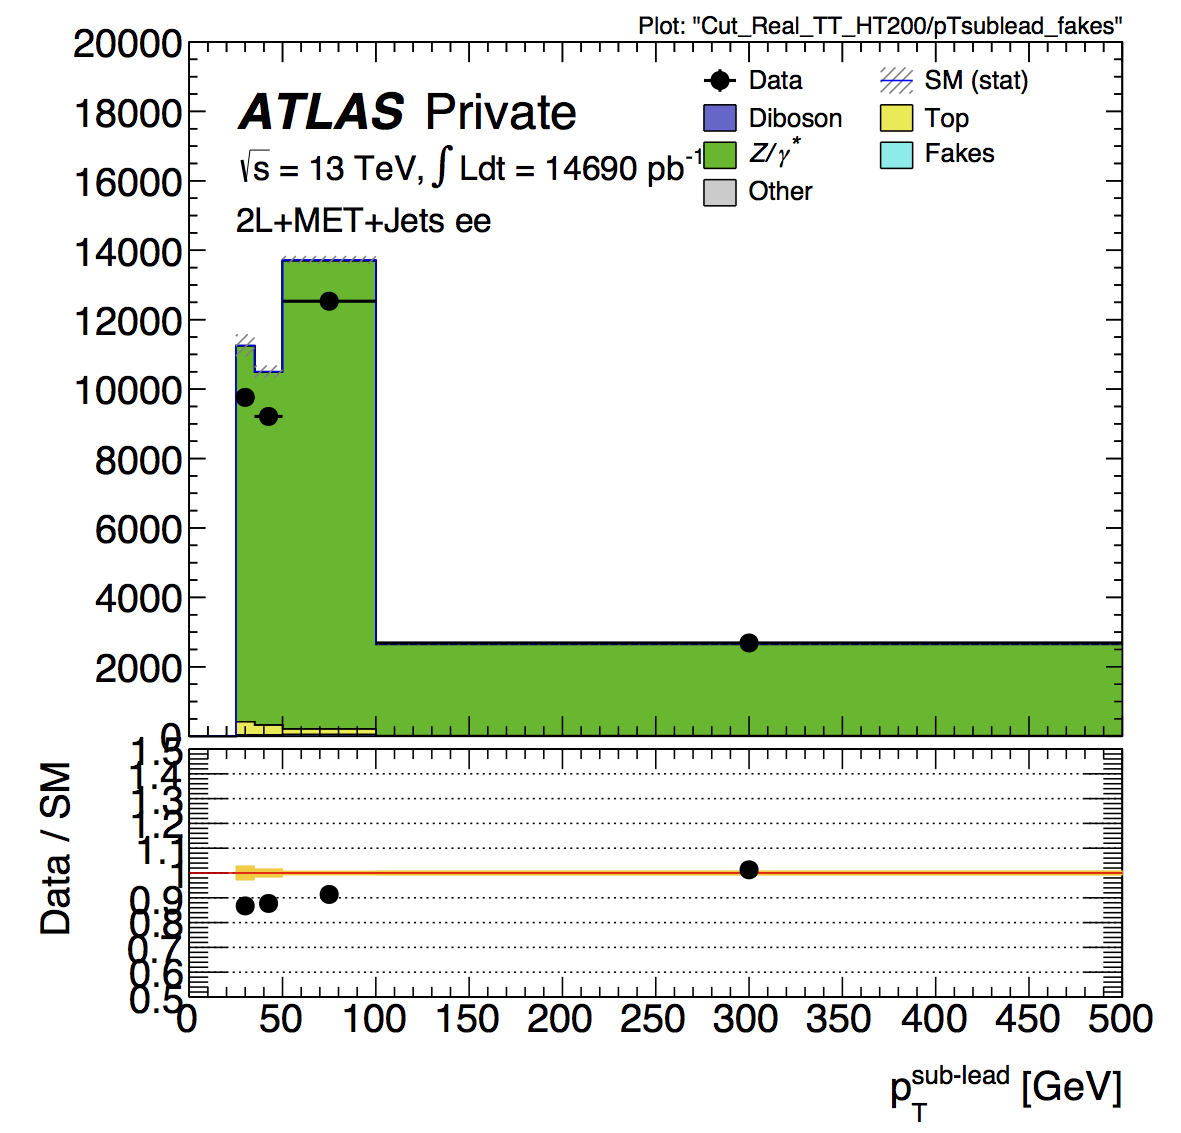
\includegraphics[width=.45\linewidth]{figures/fakes/ee-Cut_Real_TT_HT200-pTsublead_fakes-lin_2016.png}
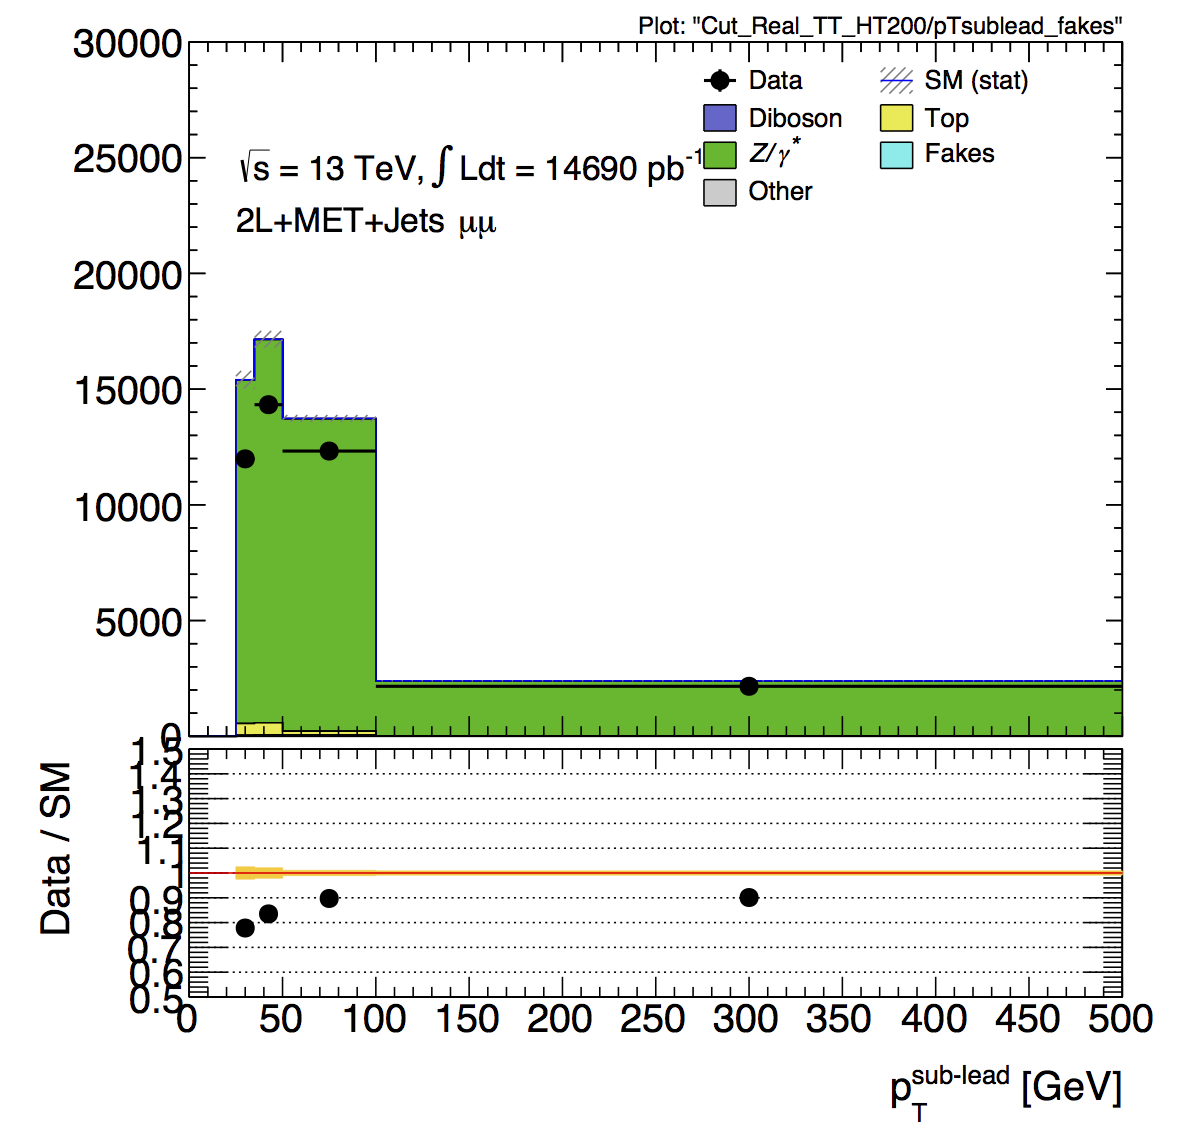
\includegraphics[width=.45\linewidth]{figures/fakes/mm-Cut_Real_TT_HT200-pTsublead_fakes-lin_2016.png}
\caption{Sub-leading lepton \pT\ for $ee$ (left) and $\mu\mu$ (right) events with two leptons passing the signal requirements in CR-real for 2016. }
\label{fig:fake_realreg}
\end{figure}
\end{centering}

The fake efficiency, $\epsilon^{fake}$, is determined using the tag-and-probe method in CR-fake, also described in \autoref{tab:regions-fakes}. This region is different from all other regions considered in this analysis because it requires same-sign leptons. Very few \ac{SM} processes genuinely produce two same-sign leptons, so this region is enhanced in fake leptons. An upper limit on \met is placed on CR-fake to limit the possible contamination from \ac{BSM} processes. According to \ac{MC}, real, prompt leptons make up about 7\% (11\%) of the baseline electron (muon) sample and about 10\% (61\%) of the signal electron (muon) sample in this region. These real lepton backgrounds are subtracted from the CR-fake yields when calculating the efficiencies. \autoref{fig:fake_fakereg} shows a comparison of data and \ac{MC} in this region.

\begin{centering}
\begin{figure}[htbp]
\centering
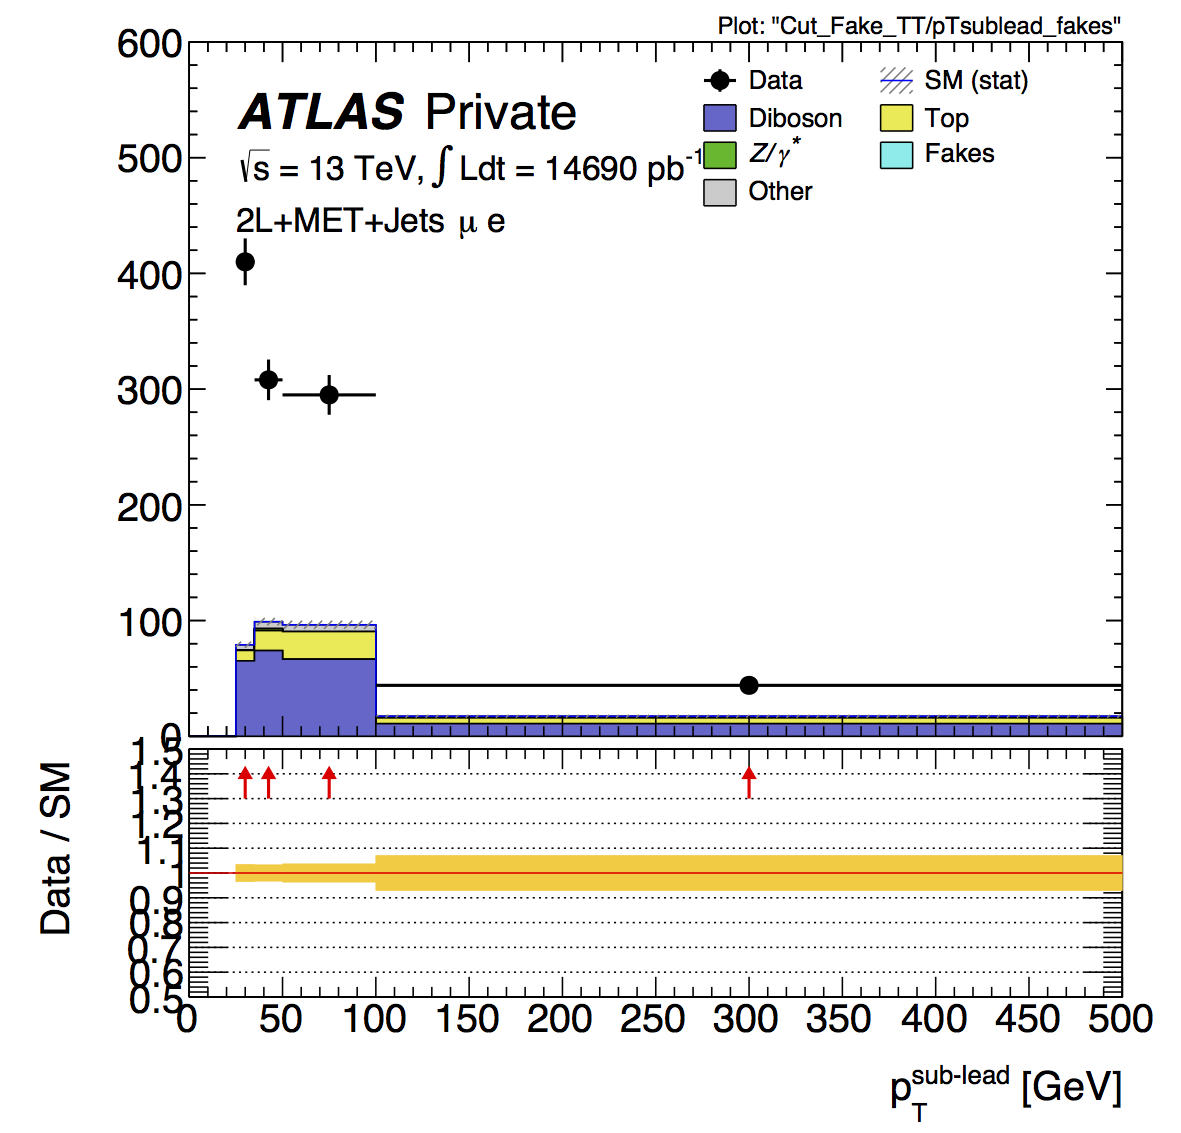
\includegraphics[width=.45\textwidth]{figures/fakes/me-Cut_Fake_TT-pTsublead_fakes-lin_2016.png}
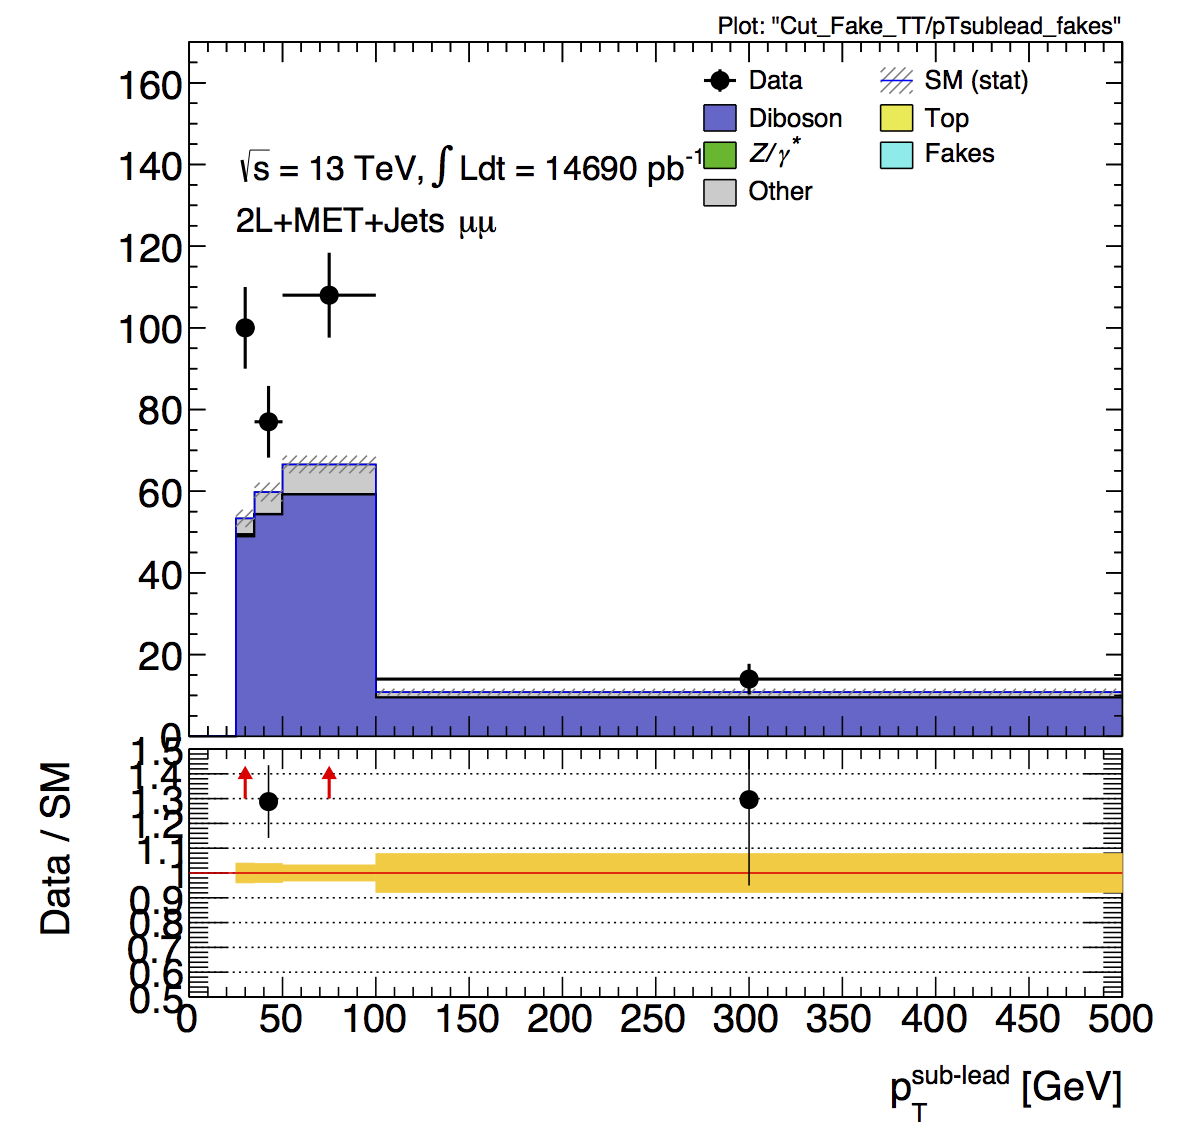
\includegraphics[width=.45\textwidth]{figures/fakes/mm-Cut_Fake_TT-pTsublead_fakes-lin_2016.png}
\caption{Sub-leading lepton \pT\ for $\mu e$ (left) and $\mu\mu$ (right) events with two leptons passing signal requirements in CR-fake for 2016.}
\label{fig:fake_fakereg}
\end{figure}
\end{centering}

This method is validated in a fakes-rich \ac{VR} with a same-sign lepton requirement, \met $\geq$ 50\gev, $\geq$ 2 jets, and a veto on \mll~on the $Z$-mass peak for same flavor channels to reduce the number of \dyjets events with mismeasured lepton charge. The results of this validation can be seen in \autoref{fig:fakes_validation}. With the systematic uncertainties, discussed in \autoref{sec:uncert_fakes}, the prediction agrees well with the data across a wide range of \mll~values. 

%TODO add this to table

\begin{centering}
\begin{figure}[!htb]
\centering
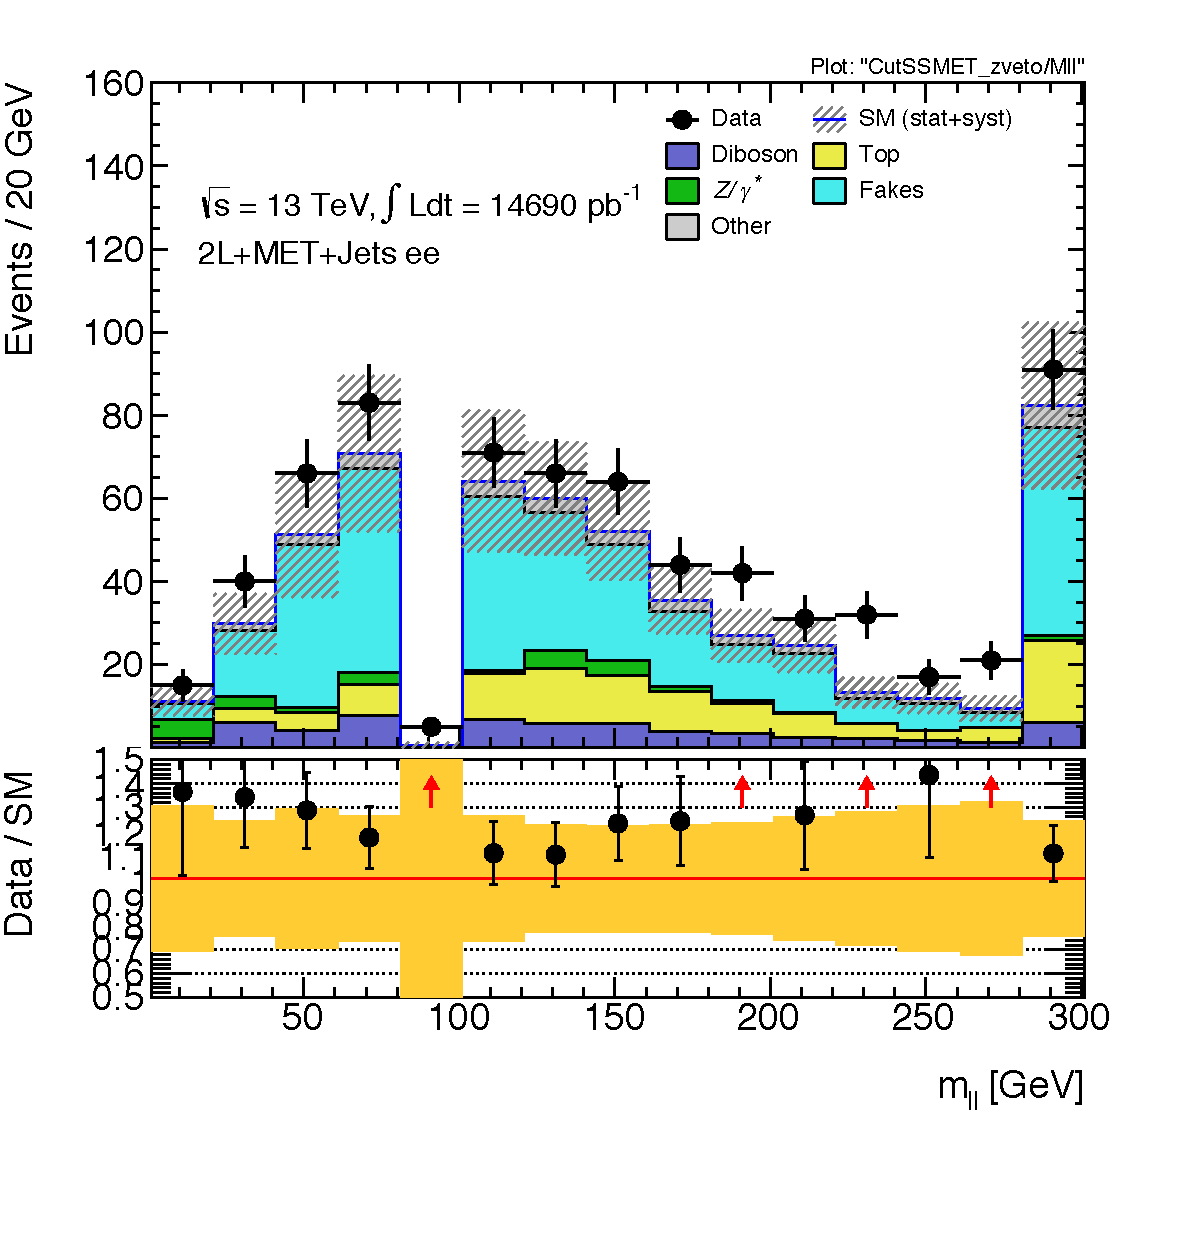
\includegraphics[width=.45\textwidth]{figures/fakes/ee-CutSSMET_zveto-Mll-lin.pdf}
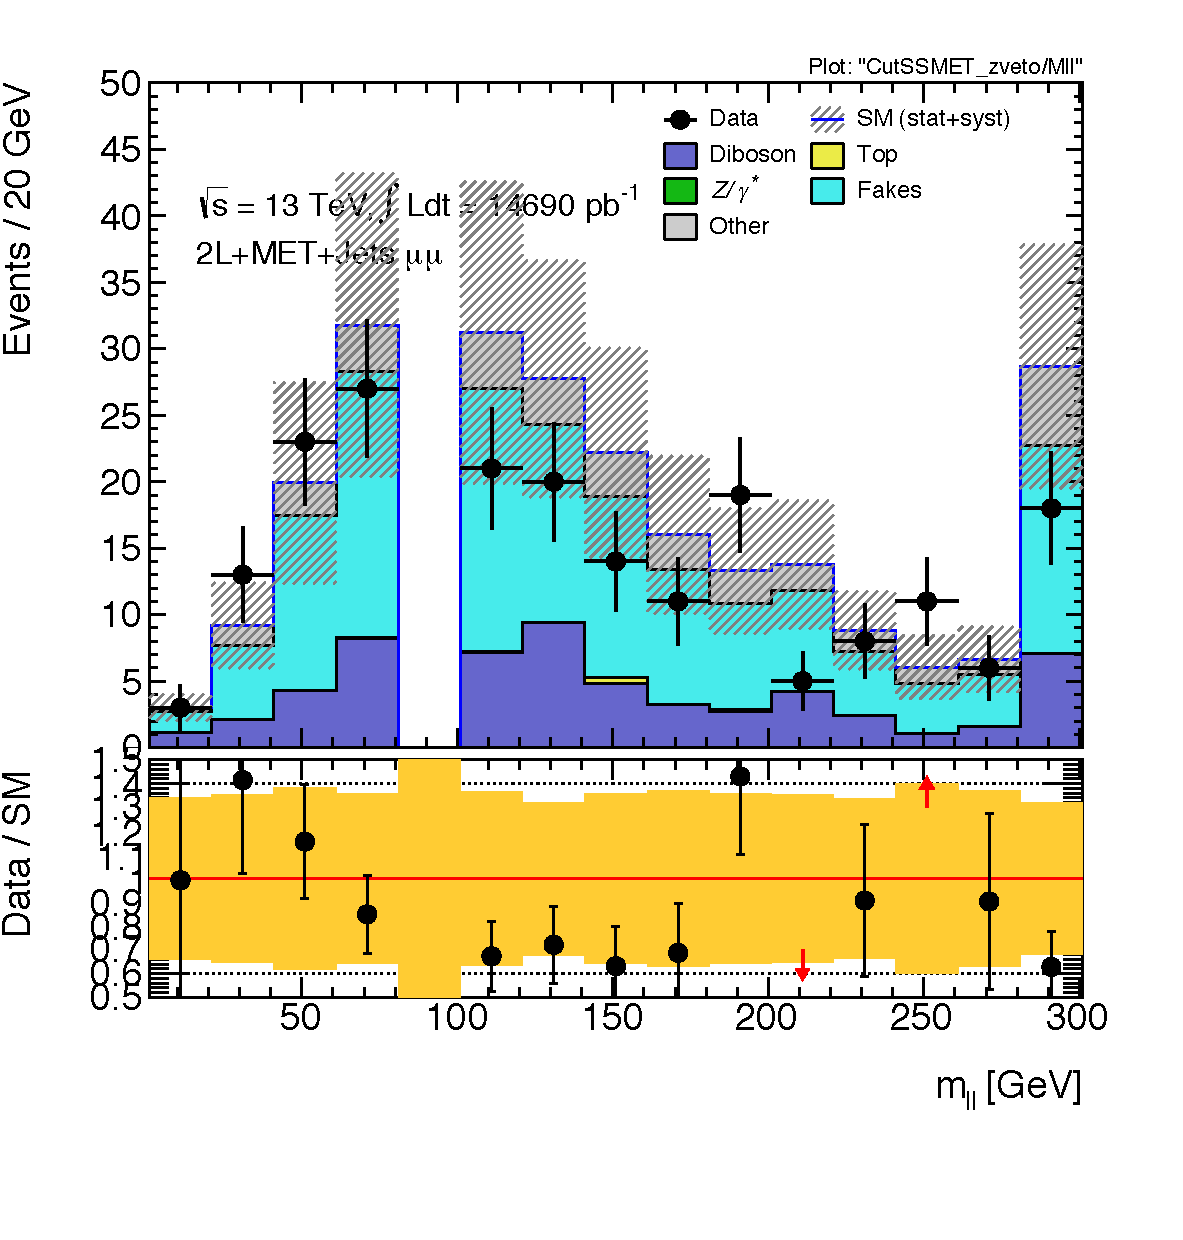
\includegraphics[width=.45\textwidth]{figures/fakes/mm-CutSSMET_zveto-Mll-lin.pdf}
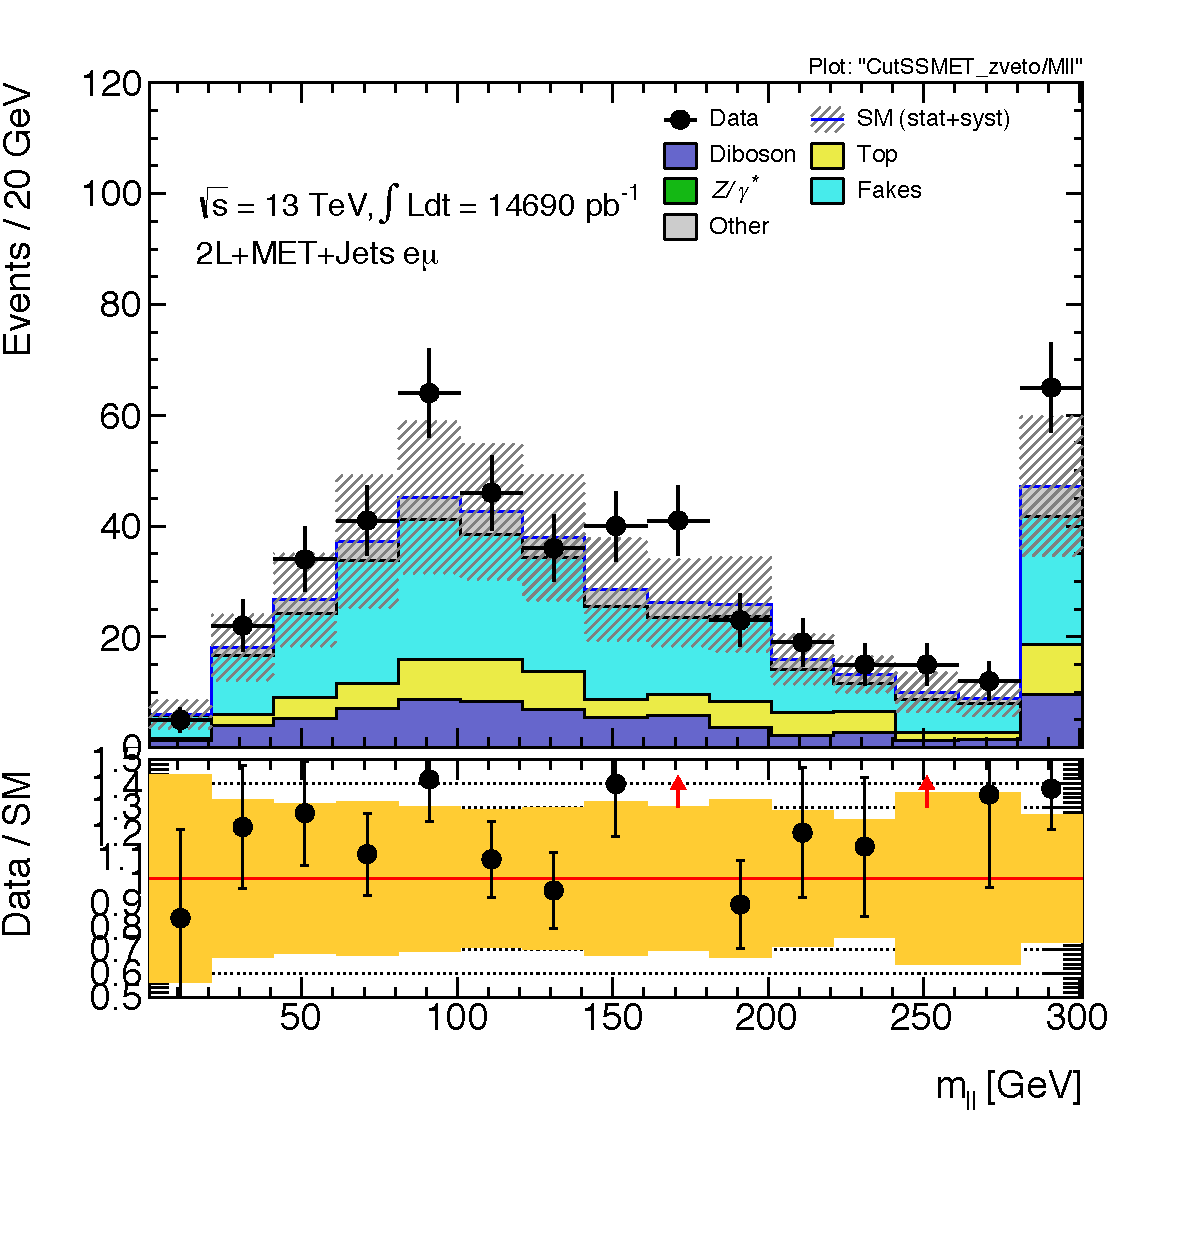
\includegraphics[width=.45\textwidth]{figures/fakes/em-CutSSMET_zveto-Mll-lin.pdf}
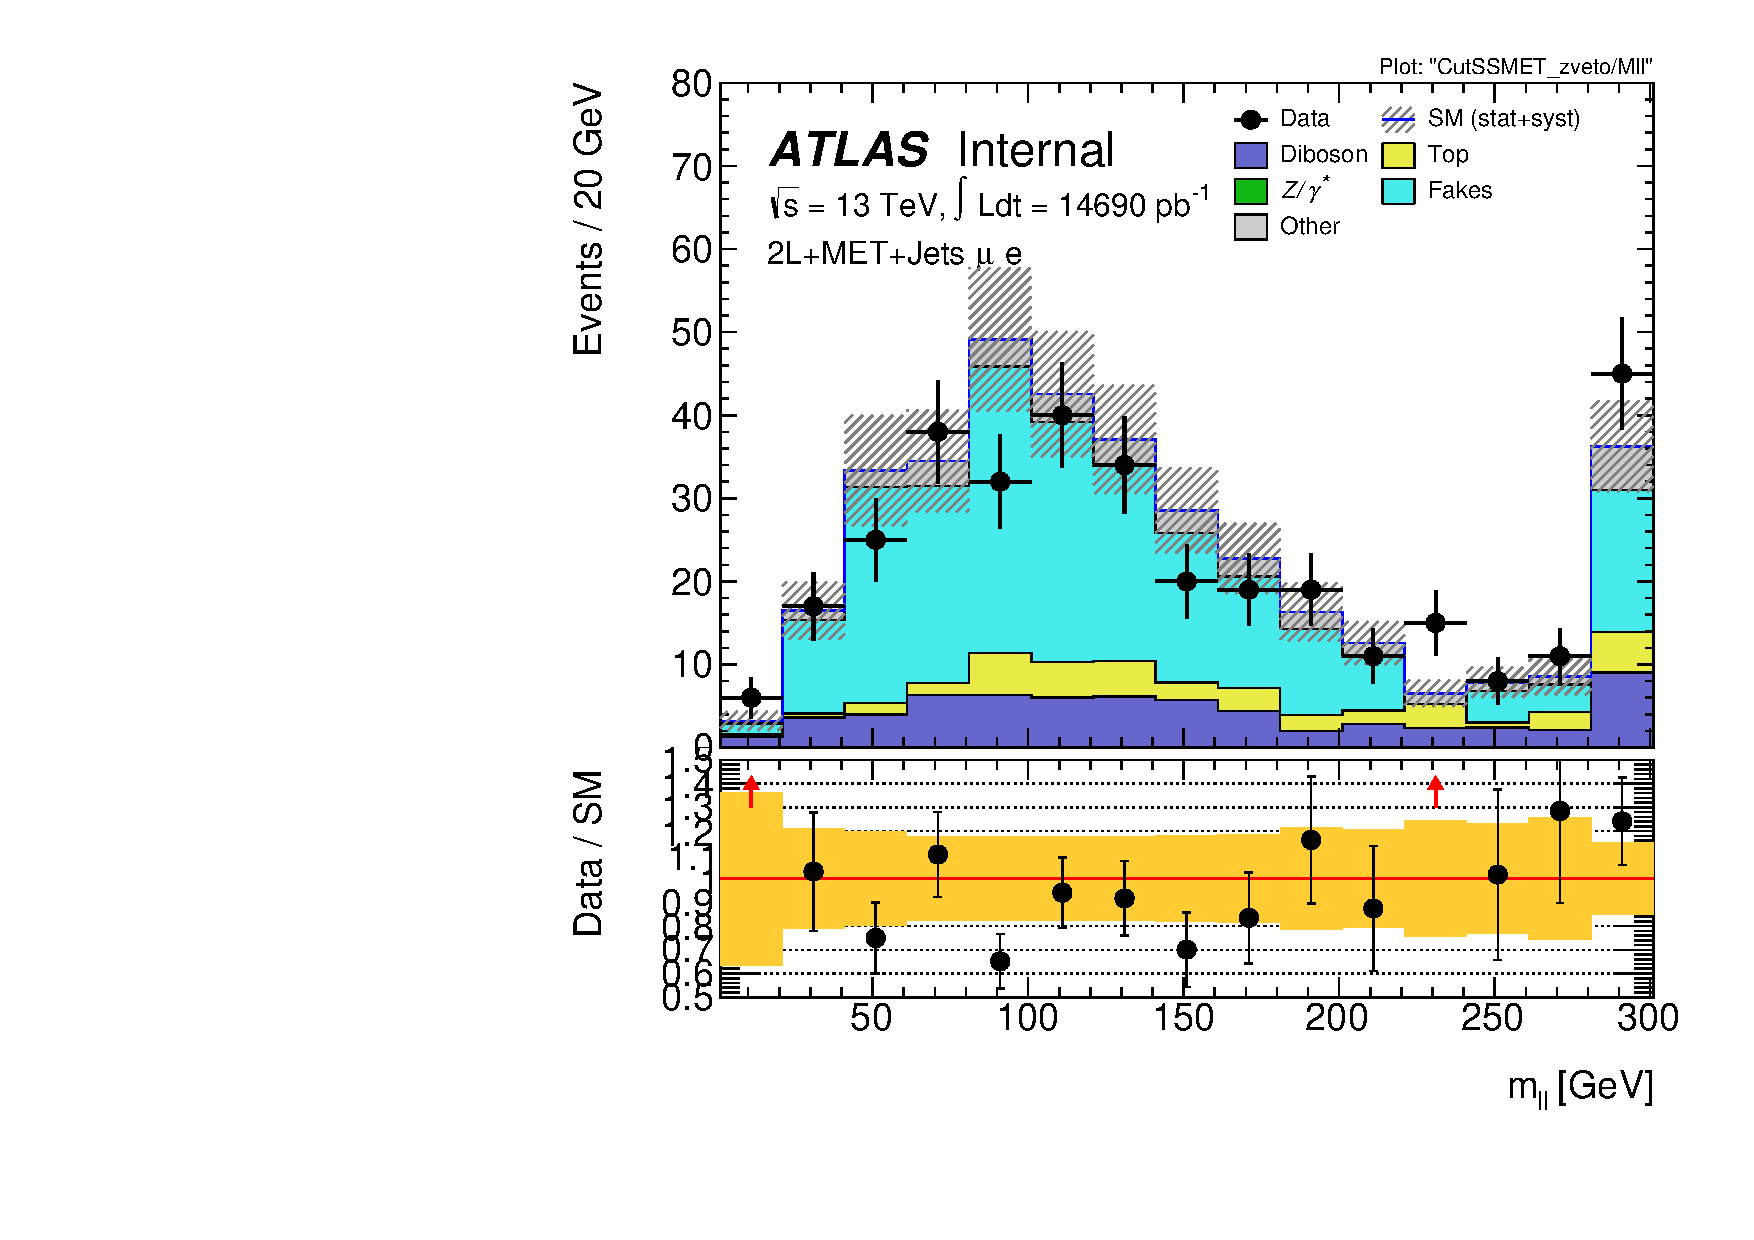
\includegraphics[width=.45\textwidth]{figures/fakes/me-CutSSMET_zveto-Mll-lin.pdf}
\caption{Same sign validation regions in the $ee$ (top left), $\mu\mu$ (top right), $e\mu$ (bottom left) and $\mu e$ (bottom right) channels combining 2015+2016 data. Uncertainty bands include both statistical and systematic uncertainties. \label{fig:fakes_validation}}
\end{figure}
\end{centering}

\section{Diboson and Rare Top Processes}
\label{sec:bg-other}

The remaining backgrounds are diboson processes (excluding $WW$, which is included in the \ac{FS} background) and rare top processes. Dibosons events make up about 30\% of the events in SRZ, while rare top process contributions are much smaller, and make up about 5\% of SRZ. Both are taken directly from \ac{MC}, with validation regions to confirm the accuracy of the prediction. 

These regions are described in \autoref{tab:regions-z}, and target different parts of these backgrounds. VR-ZZ is a four-lepton region designed to select a very pure sample of $ZZ$ events. VR-WZ requires three leptons and makes cuts on $m_\mathrm{T}$, the transverse mass\footnote{More specifically, this transverse mass is formed by the \met and the lepton which is not assigned to the $Z$ boson decay. The leptons associated with the $Z$ boson are the opposite sign pair with the invariant mass closest to that of the $Z$ boson. }, 
and \met in order to select mostly $WZ\rightarrow lll\nu$ events. Both of these regions veto events with $b$-jets in order to reduce \ttbar backgrounds. VR-3L is similar to VRS, but loosens the \HT and \met cuts and requires at least three leptons. This region is designed to target any $\geq3$-lepton process in a region as kinematically close to SRZ as possible while still maintaining enough events to validate. The makeups of these multilepton validation regions, as well as VRS, are shown in \autoref{tab:VRresults}.



\begin{table}[!htb]
\begin{center}
\setlength{\tabcolsep}{0.0pc}
\resizebox{1\textwidth}{!}{
\begin{tabular*}{\textwidth}{@{\extracolsep{\fill}}lrrrr}
\noalign{\smallskip}\hline\noalign{\smallskip}
                                                                             & VRS            & VR-WZ        & VR-ZZ          & VR-3L   \\[-0.05cm]
\noalign{\smallskip}\hline\noalign{\smallskip}
Observed events                                                              & $236$            & $698$        & $132$          & $32$ \\
\noalign{\smallskip}\hline\noalign{\smallskip}
%Total expected background events                                             & $223.92 \pm 40.84$   &   $612.97\pm8.65$   &    $139.29\pm4.95$    &    $34.52\pm1.39$ \\
% here the total background uncertainty is updated to the quadrature sum of each bkg uncertainty
Total expected background                                             & $224 \pm 41$   &   $613\pm66$   &    $139\pm25$    &    $35\pm10$ \\
\noalign{\smallskip}\hline\noalign{\smallskip}
  Flavour-symmetric             & $99\pm8$   &   -                &    -                 &    -              \\
  $WZ/ZZ$ events                                                             & $27\pm13$  &   $573\pm66$ &    $139\pm25$        &    $25\pm10$ \\
  Rare top events                                                            & $11\pm3$   &   $14\pm3$   &    $0.44\pm0.11$     &    $9.1\pm2.3$  \\
  \dyjets\ events                                                            & $84\pm37$  &   -                &    -                 &    -              \\
  Fake lepton events                                                         & $4\pm4$    &   $26\pm6$   &    -                 &    $0.6\pm0.3$  \\
 \noalign{\smallskip}\hline\noalign{\smallskip}
\end{tabular*}
} % end of resizebox
\end{center}
\caption{Yields in validation regions. In VRS, data-driven background estimates are used for \dyjets, fakes, and \ac{FS} processes. All other backgrounds are taken from \ac{MC}, including all backgrounds in the multi-lepton \ac{VR}s. Uncertainties include statistical and systematic components. }
\label{tab:VRresults}
\end{table}


To confirm that the kinematics are well modeled in the diboson validation regions, distributions of \HT and $Z$ boson \pt are shown in \ac{MC} and data. Figures \ref{fig:diboson_wz} shows these distributions for VR-WZ, and \autoref{fig:diboson_zz} shows these distributions for VR-ZZ. 


\begin{centering}
\begin{figure}[htbp]
\centering
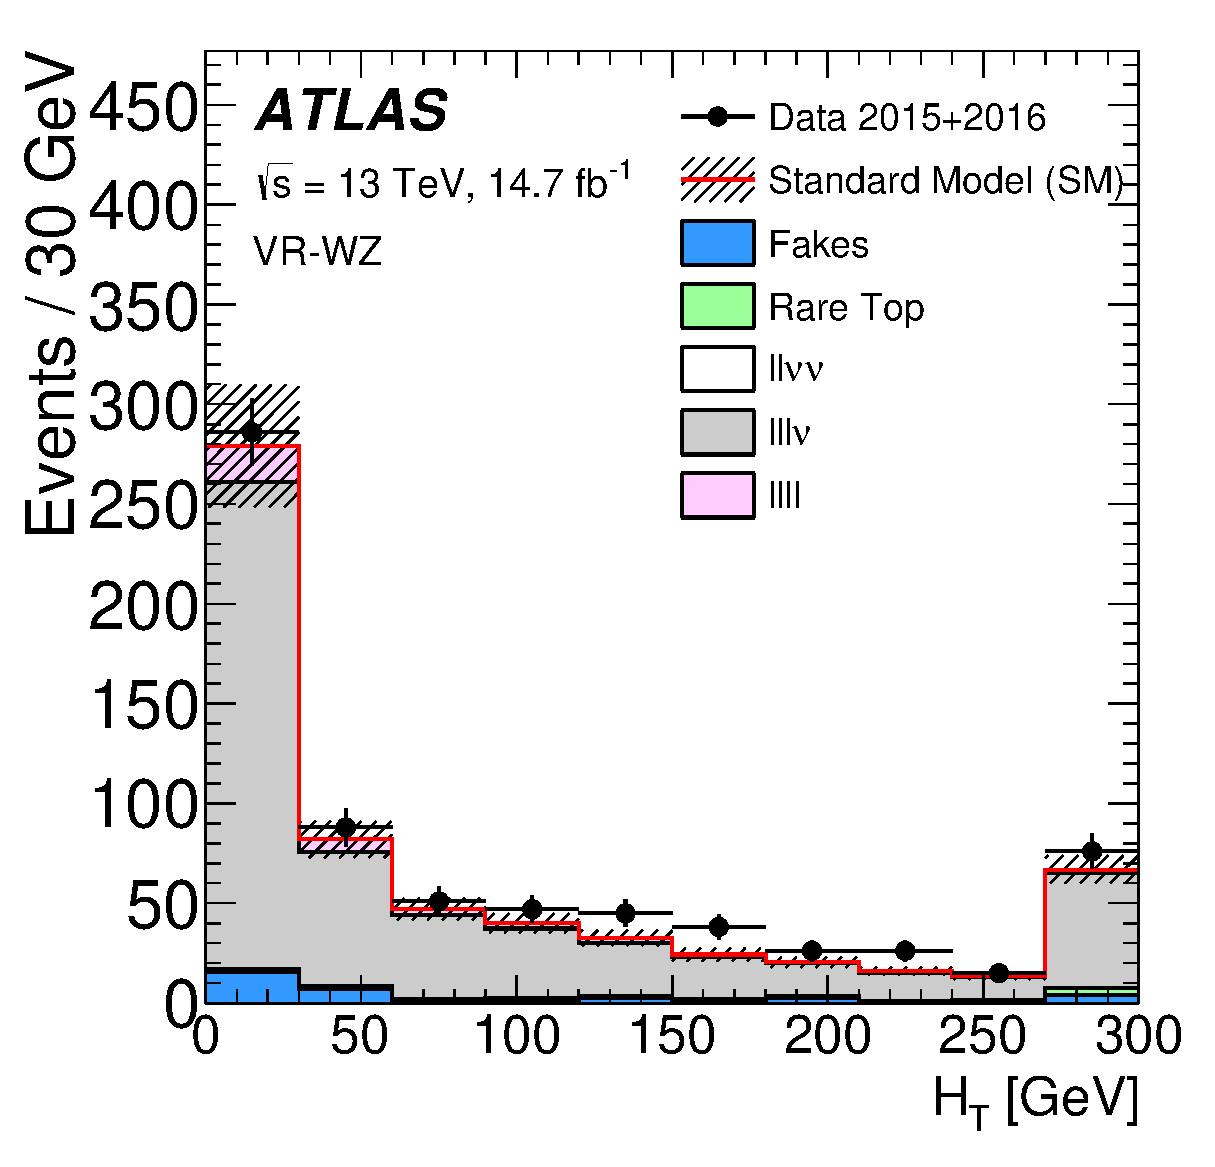
\includegraphics[width=.9\textwidth]{figures/dibosons/figaux_11a.eps}
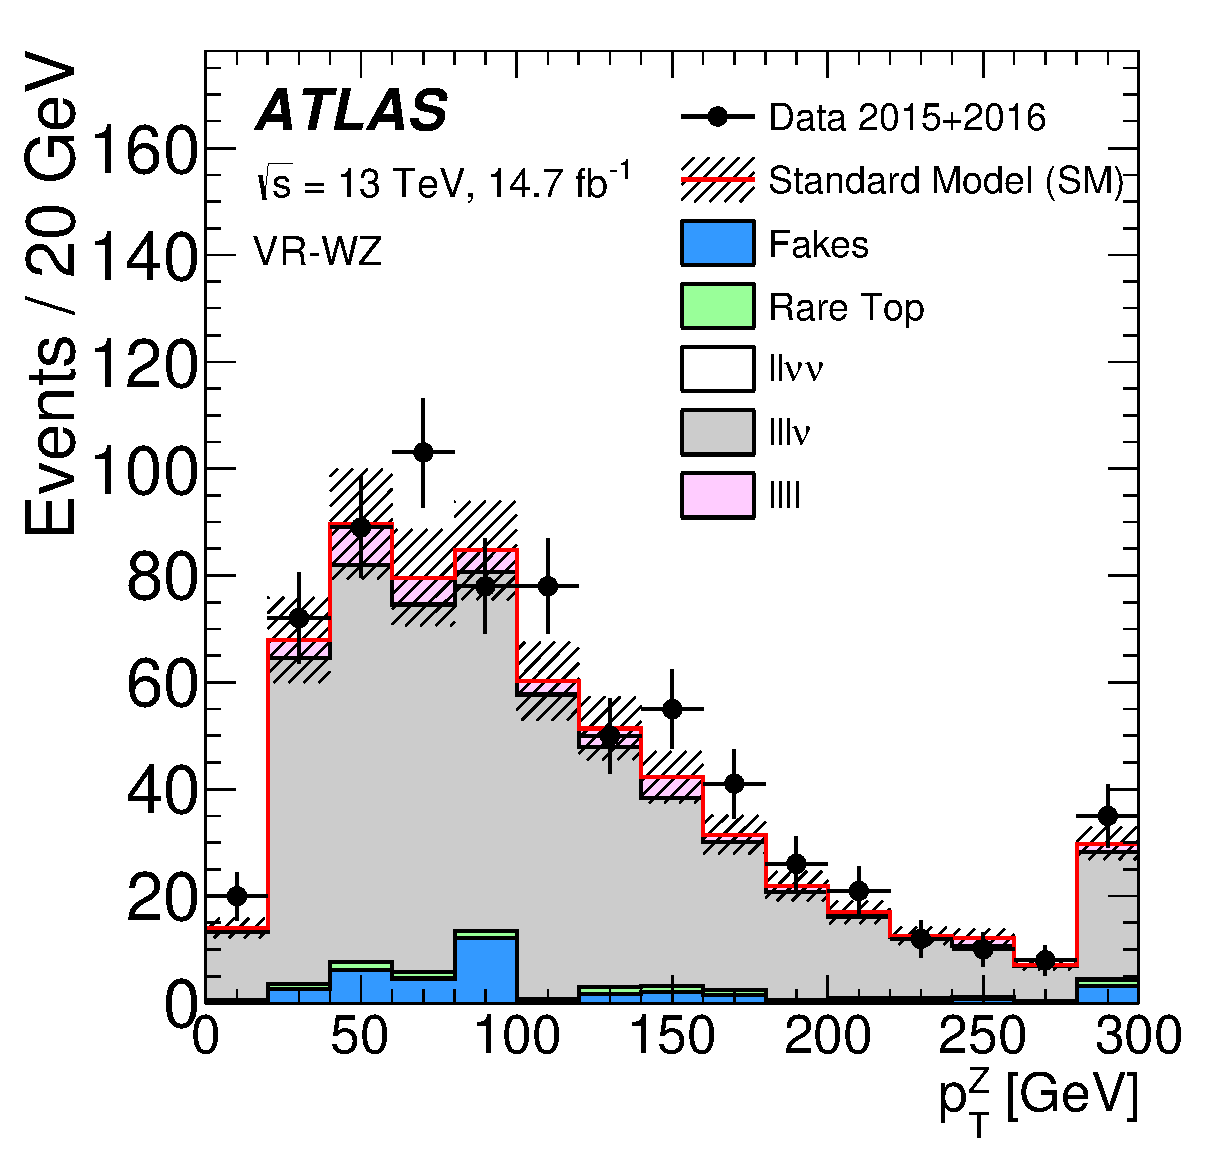
\includegraphics[width=.9\textwidth]{figures/dibosons/figaux_11b.eps}
\caption{\HT (top) and $Z$ boson \pt (bottom) distribtuions of data and \ac{MC} in VR-WZ. The hashed bands include the MC statistical uncertainties and theoretical uncertainties on the diboson background. The last bin contains the overflow. \label{fig:diboson_wz}}
\end{figure}
\end{centering}

\begin{centering}
\begin{figure}[htbp]
\centering
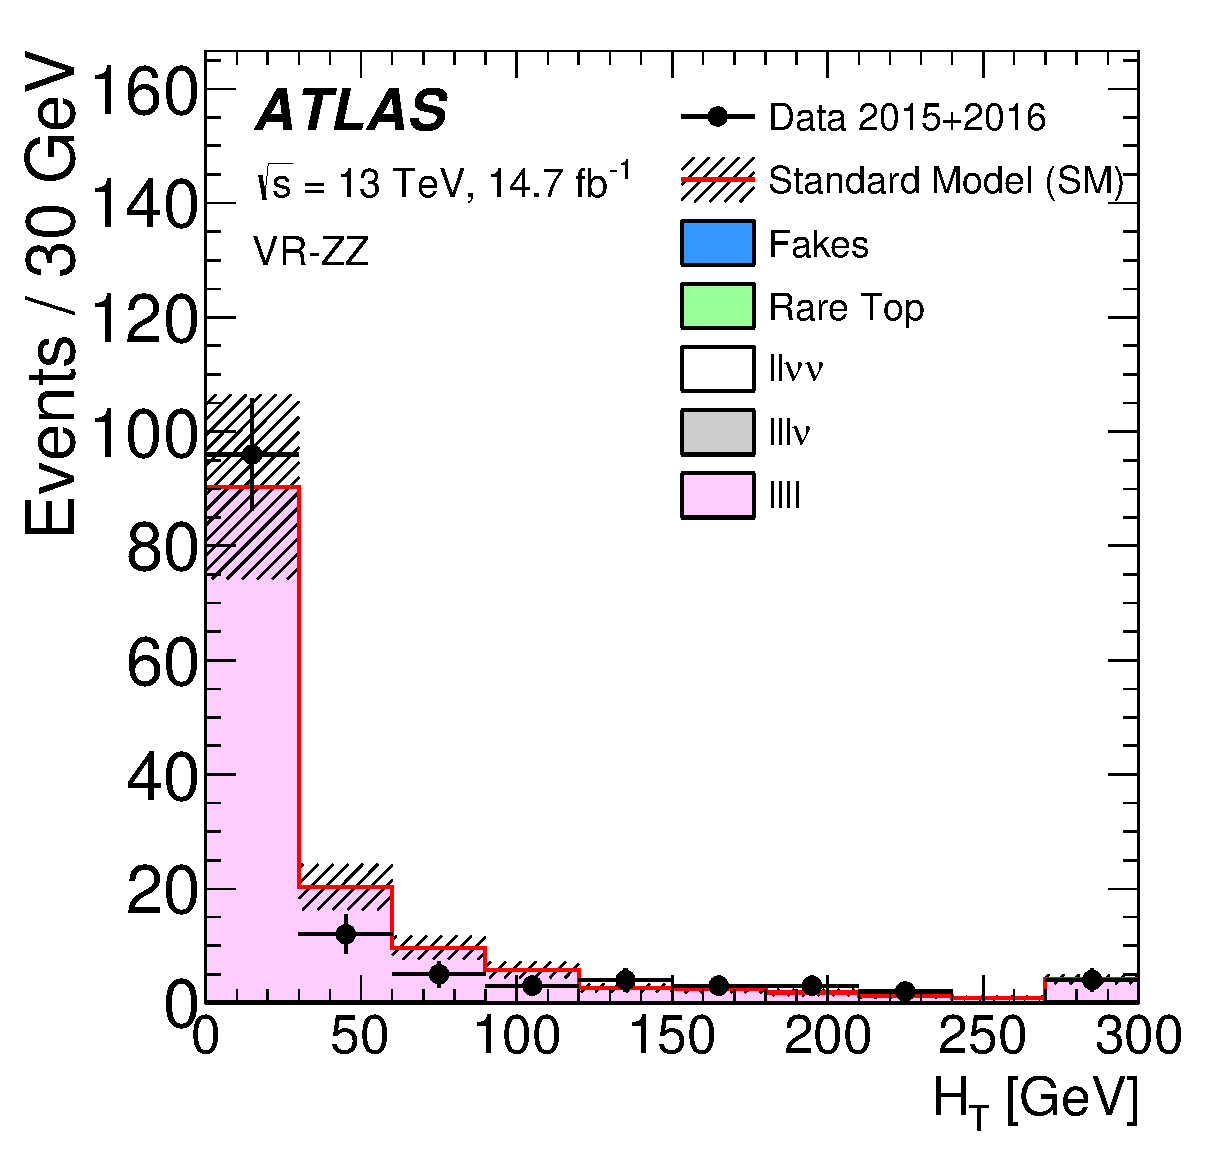
\includegraphics[width=.9\textwidth]{figures/dibosons/figaux_11c.eps}
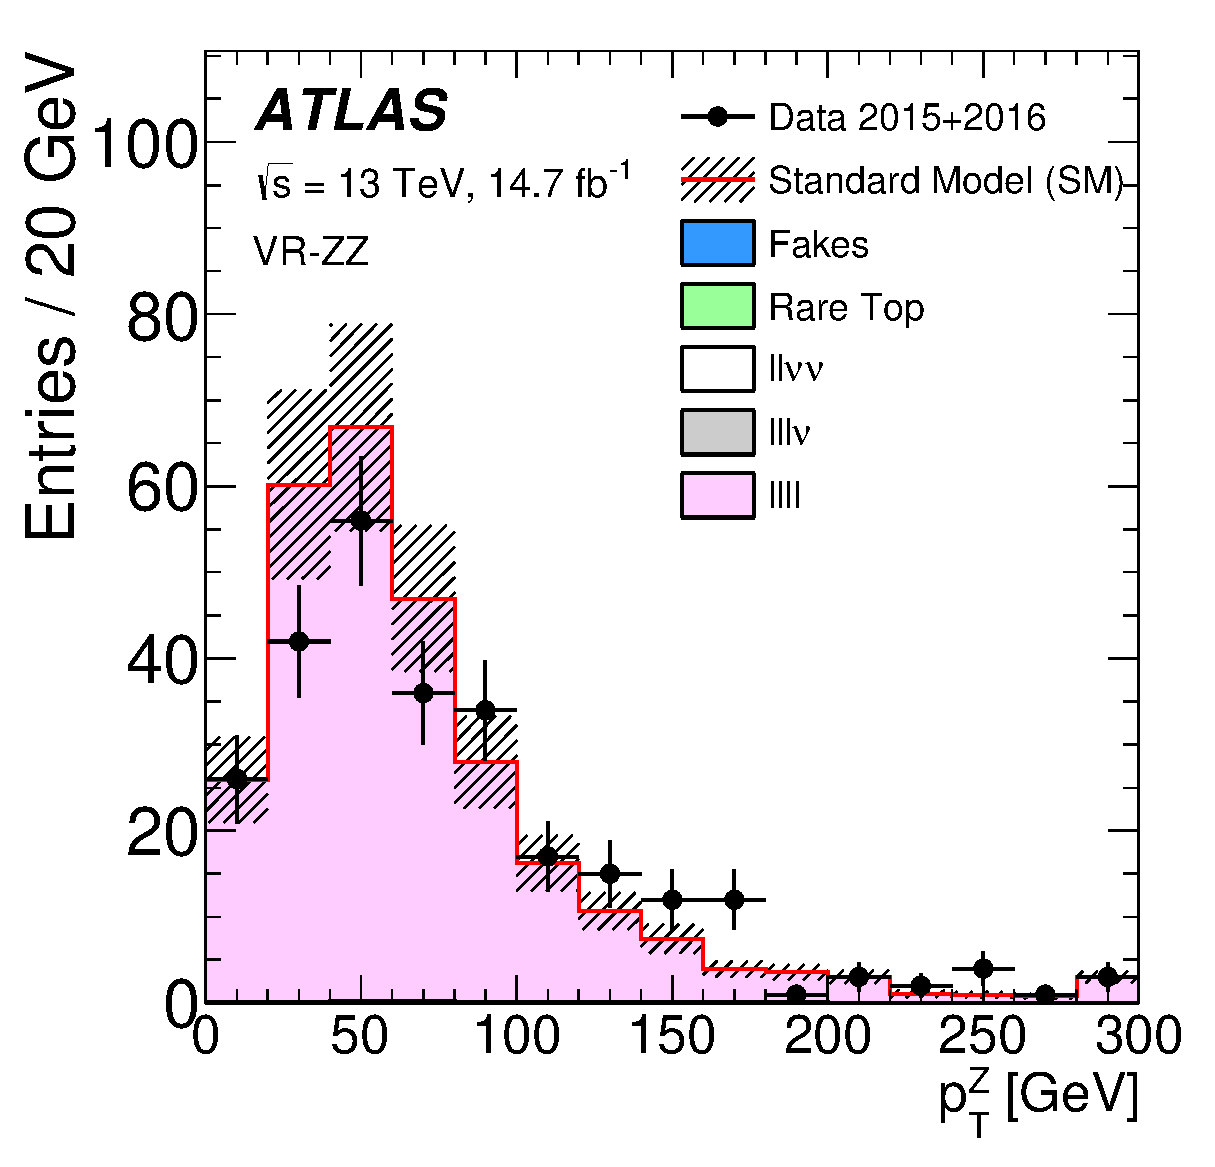
\includegraphics[width=.9\textwidth]{figures/dibosons/figaux_11d.eps}
\caption{\HT (top) and $Z$ boson \pt (bottom) distribtuions of data and \ac{MC} in VR-ZZ. The hashed bands include the MC statistical uncertainties and theoretical uncertainties on the diboson background. The last bin contains the overflow. \label{fig:diboson_zz}}
\end{figure}
\end{centering}

%\begin{centering}
%\begin{figure}[htbp]
%\centering
%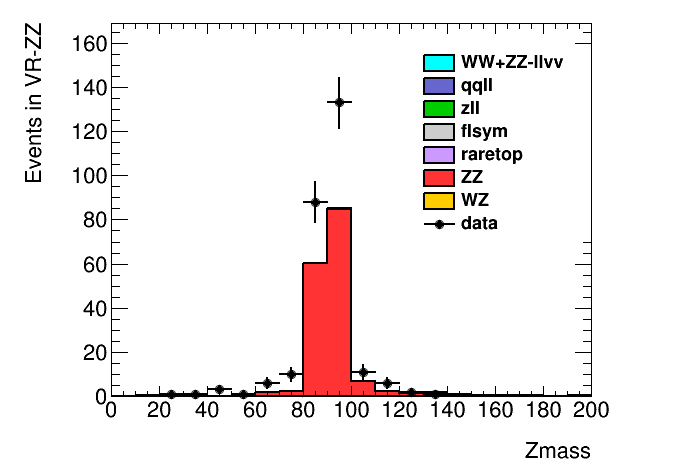
\includegraphics[width=.9\textwidth]{figures/dibosons/ZZ_Zmass.png}
%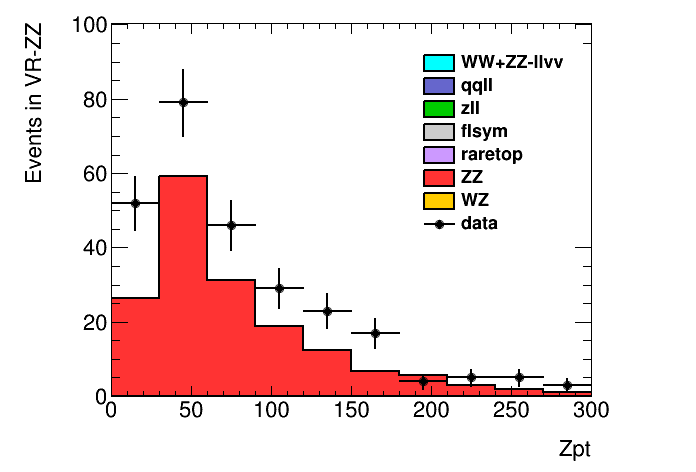
\includegraphics[width=.9\textwidth]{figures/dibosons/ZZ_Zpt.png}

%\caption{Distribtuions in VR-WZ. On the top, mass of the $Z$ bosons in the event, and on the bottom, \pT of the $Z$ bosons. \label{fig:diboson_zz}}
%\end{figure}
%\end{centering}

